% Ce fichier main.tex est le fichier principal \`{a} partir duquel tout est g\'{e}n\'{e}r\'{e}
% This file is the main file where the final document is generated
\documentclass{these-dbl}


\usepackage{amsmath,amsfonts,amssymb,amsthm}
\usepackage{empheq}
\usepackage{subcaption}
\usepackage{enumerate}  % lists with (i)
\usepackage{yhmath}     % for very wide hats
\usepackage{ifthen}

% \usepackage[
%   backend=biber,
%   style=alphabetic, % `numeric` to count 
%   sorting=nyt, 
%   maxalphanames=99, 
%   maxbibnames=99,
%   doi=false,isbn=false,url=false
% ]{biblatex}
\addbibresource{bibJellyRoll.bib}

\NewBibliographyString{toappear}
\DefineBibliographyStrings{english}{%
  toappear = {to appear in},
}
\DefineBibliographyStrings{french}{%
  toappear = {à paraître dans},
}

\renewbibmacro*{in:}{%
  \iffieldundef{pubstate}
    {}
    {\printfield{pubstate}%
     \setunit{\addspace}%
     \clearfield{pubstate}}%
%   \printtext{%
%     \intitlepunct}%
    }


%----------------------------------------------------------
% Temporary packages
\usepackage{lipsum}
\usepackage[textwidth=3.7cm]{todonotes}
\geometry{inner=1cm, outer=4.5cm}
\setlength{\marginparwidth}{3.7cm}
%----------------------------------------------------------

\newtheorem{theorem}{Theorem}[section]
\newtheorem{proposition}[theorem]{Proposition}
\newtheorem{definition}[theorem]{Definition}
\newtheorem{remark}[theorem]{Remark}
\newtheorem{corollary}[theorem]{Corollary}
\newtheorem{lemma}[theorem]{Lemma}
\newtheorem{assumption}[theorem]{Assumption}
\newtheorem{property}[theorem]{Property}

\newtheorem*{theorem*}{Theorem}
\newtheorem*{FRtheorem*}{Théorème}
\newtheorem*{proposition*}{Proposition}
\newtheorem*{definition*}{Definition}
\newtheorem*{FRdefinition*}{Définition}
\newtheorem*{remark*}{Remark}
\newtheorem*{FRremark*}{Remarque}
\newtheorem*{corollary*}{Corollary}
\newtheorem*{lemma*}{Lemma}
\newtheorem*{assumption*}{Assumption}
\newtheorem*{FRassumption*}{Hypothèse}
\newtheorem*{property*}{Property}
\newtheorem*{FRproperty*}{Propriété}



\newcommand{\eps}{\ensuremath{\varepsilon}}
\newcommand{\pa}{\ensuremath{\partial}}
\newcommand{\dd}{\ensuremath{\mathrm{d}}}
\newcommand{\rk}[1]{^{[#1]}}
\newcommand{\bigO}{\mathcal{O}}
\newcommand{\Dt}{\ensuremath{\Delta t}}

\newcommand{\setN}{\mathbb{N}}
\newcommand{\setZ}{\mathbb{Z}} 
\newcommand{\setQ}{\mathbb{Q}}
\newcommand{\setR}{\mathbb{R}} 
\newcommand{\setC}{\mathbb{C}}
\newcommand{\setT}{\mathbb{T}}
\newcommand{\setK}{\mathcal{K}}

\newcommand{\R}{\mathbb{R}} \newcommand{\C}{\mathbb{C}}
\newcommand{\Z}{\mathbb{Z}} \newcommand{\N}{\mathbb{N}}
\newcommand{\T}{\mathbb{T}}

\newcommand{\RR}{\rangle}
\newcommand{\LL}{\langle}
\newcommand{\bRR}{\big \rangle}
\newcommand{\bLL}{\big \langle}
\newcommand{\BRR}{\Big \rangle}
\newcommand{\BLL}{\Big \langle}

\newcommand{\among}[2]{\begin{pmatrix} #1 \\ #2 \end{pmatrix}}

% triple norm 
\newcommand{\vertiii}[1]{{\left\vert\kern-0.25ex\left\vert\kern-0.25ex\left\vert #1 %
    \right\vert\kern-0.25ex\right\vert\kern-0.25ex\right\vert}}

\DeclareMathOperator{\id}{id}
\DeclareMathOperator{\tr}{tr}
\DeclareMathOperator{\Tr}{tr}
\DeclareMathOperator{\err}{err}

\makeatletter
\newcommand*\bigcdot{\mathpalette\bigcdot@{.5}}
\newcommand*\bigcdot@[2]{\mathbin{\vcenter{\hbox{\scalebox{#2}{$\m@th#1\bullet$}}}}}
\makeatother


%--------------------------------
% Pour Chap. III
\newcommand{\K}{\mathcal{K}}
\newcommand{\ul}[1]{\underline{#1}}
\newcommand{\ol}[1]{\overline{#1}}

\newcommand{\e}{\varepsilon}
\newcommand{\ee}{^{\e}}
\newcommand{\ie}{_{\e}}
\newcommand{\eeps}{\ee}
\newcommand{\ieps}{\ie}
\newcommand{\inveps}{\frac{1}{\eps}}

\newcommand{\lp}{\big(}\newcommand{\rp}{\big)}
\newcommand{\LP}{\Big(}\newcommand{\RP}{\Big)}
\newcommand{\Langle}{\big\langle}
\newcommand{\Rangle}{\big\rangle}
\newcommand{\D}{\mathrm{d}}

\newcommand{\dpt}{\partial_t}
\newcommand{\dptau}{\partial_{\tau}}
\newcommand{\dptheta}{\partial_{\theta}}
\newcommand{\dpu}{\partial_{u}}
\newcommand{\dpx}{\partial_{x}}
\newcommand{\dpz}{\partial_{z}}
\newcommand{\dpy}{\partial_{y}}


% Remplir les metadonnees du pdf
% Fill the pdf metadata
\hypersetup{
    pdfauthor   = {Léopold Trémant},
    pdftitle    = {Th\`{e}se de doctorat de L\'{e}opold Tr\'{e}mant},
    pdfsubject  = {Th\`{e}se de doctorat de L\'{e}opold Tr\'{e}mant},
    pdfkeywords = {TODO},
}

\geometry{vmargin=4.0cm}

% Spécifier vos fichiers de bibliographie
% Specify you bibliography files here
\addbibresource{./biblio/biblio.bib}

\begin{document}

% Page de garde avec commande \maketitle
% Front cover calling \maketitle
% La page de garde est en français
% The front cover is in French
\selectlanguage{french}

% Inclure les infos de chaque établissement
% Include each institution data
\input{./Couverture-these/liste-ecoles-etablissements.tex}

% Inclure infos de l'école doctorale
% Include doctoral school data
% (3M ALL BS DSP EDGE EGAAL ELICC MathSTIC SML SPI STT)
\ecoledoctorale{MathSTIC}

% Inclure infos de l'établissement
% Include institution data
\etablissement{UR1}

%Inscrivez ici votre sp\'{e}cialit\'{e} (voir liste des sp\'{e}cialit\'{e}s sur le site de votre \'{e}cole doctorale)
%Indicate the domain (see list of domains in your ecole doctorale)
\spec{Mathématiques et Interactions}

%Attention : le pr\'{e}nom doit être en minuscules (Jean) et le NOM en majuscules (BRITTEF) 
%Attention : the first name in small letters and the name in Capital letters 
\author{L\'{e}opold \textsc{Tr\'{e}mant}}

% Donner le titre complet de la th\`{e}se, \'{e}ventuellement le sous titre, si n\'{e}cessaire sur plusieurs lignes 
%Give the complete title of the thesis, if necessary on several lines
\title{M\'ethodes d'analyse asymptotique et d'approximation num\'erique}
\lesoustitre{Problèmes d'évolution multi-\'echelles de type oscillatoire ou dissipatif}

%Indiquer la date et le lieu de soutenance de la th\`{e}se 
%indicates the date and the place of the defense 
\date{« date »}
\lieu{« Lieu »}

%Indiquer le nom du (ou des) laboratoire (s) dans le(s)quel(s) le travail de th\`{e}se a \'{e}t\'{e} effectu\'{e}, indiquer aussi si souhait\'{e} le nom de la (les) facult\'{e}(s) (UFR, \'{e}cole(s), Institut(s), Centre(s)...), son (leurs) adresse(s)... 
%Indicates the name (or names) of research laboratories where the work has been done as well as (if desired) the names of faculties (UFR, Schools, institution...
\uniterecherche{« voir liste sur le site de votre \'{e}cole doctorale »}

%Indiquer le Numero de th\`{e}se, si cela est opportun, ou laisser vide pour faire disparaitre cet ligne de la couverture
%Indicate the number of the thesis if there is one. otherwise leave empty so the line disappeurs on the cover
\numthese{} % \numthese{}

%Indiquer le Pr\'{e}nom en minuscules et le Nom en majuscules, le titre de la personne et l’\'{e}tablissement dans lequel il effectue sa recherche  
%Indicates the first name on small letters and the Names on capital letters, the person's title and the institution where he/she belongs to.
%Exemples :  Examples :
%%%- Professeur, Universit\'{e} d’Angers 
%%%- Chercheur, CNRS, \'{e}cole Centrale de Nantes 
%%%-  Professeur d’universit\'{e} – Praticien Hospitalier, Universit\'{e} Paris V  
%%%-  Maitre de conf\'{e}rences, Oniris 
%%%- Charg\'{e} de recherche, INSERM, HDR, Universit\'{e} de Tours  
 %S’il n’y a pas de co-direction, faire disparaitre cet item de la couverture  
 %In there is no co-director, remove the item from the cover
\jury{
{\normalTwelve \textbf{Rapporteurs avant soutenance :}}\\ \newline
\footnotesizeTwelve
\begin{tabular}{@{}ll}
Pr\'{e}nom NOM & Fonction et \'{e}tablissement d'exercice \\
Pr\'{e}nom NOM & Fonction et \'{e}tablissement d'exercice \\
Pr\'{e}nom NOM & Fonction et \'{e}tablissement d'exercice \\
\end{tabular}

\vspace{\baselineskip}
{\normalTwelve \textbf{Composition du Jury :}}\\
{\fontsize{9.5}{11}\selectfont {\textcolor{red}{\textit{Attention, en cas d’absence d’un des membres du Jury le jour de la soutenance, la composition du jury doit être revue pour s’assurer qu’elle est conforme et devra être répercutée sur la couverture de thèse}}}}\\ \newline
\footnotesizeTwelve
\begin{tabular}{@{}lll}

Pr\'{e}sident :        & Pr\'{e}nom NOM & Fonction et \'{e}tablissement d'exercice \textit{(à préciser après la soutenance)} \\
Examinateurs :         & Pr\'{e}nom NOM & Fonction et \'{e}tablissement d'exercice \\
                       & Pr\'{e}nom NOM & Fonction et \'{e}tablissement d'exercice \\
                       & Pr\'{e}nom NOM & Fonction et \'{e}tablissement d'exercice \\
                       & Pr\'{e}nom NOM & Fonction et \'{e}tablissement d'exercice \\
Dir. de th\`{e}se :    & Pr\'{e}nom NOM & Fonction et \'{e}tablissement d'exercice \\
Co-dir. de th\`{e}se : & Pr\'{e}nom NOM & Fonction et \'{e}tablissement d'exercice \textit{(si pertinent)} \\
\end{tabular}

\vspace{\baselineskip}
{\normalTwelve \textbf{Invit\'{e}(s) :}}\\ \newline
\footnotesizeTwelve
\begin{tabular}{@{}ll}
Pr\'{e}nom NOM & Fonction et \'{e}tablissement d'exercice \\
\end{tabular}
}


\maketitle


% Sélectionner la langue du contenu suivant cette ligne
% Select the content language following this line
\selectlanguage{french}

% Inclusion du chapitre remerciement
% Input acknowledgement chapter
\clearemptydoublepage
\chapter*{Remerciements}


En premier lieu, je tiens à remercier mes parents. Malgré votre incompréhension de mon sujet de thèse, vous êtes restés curieux non seulement de l'avancée de mes recherches, mais aussi de certains concepts mathématiques sous-jacents que j'expliquais pourtant laborieusement. Merci pour votre soutien permanent, pour les bouffées d'air frais à la maison, pour les conseils de pédagogie, les coups de pied au fesses pour les démarches que je laissais traîner, et surtout pour les valeurs que vous m'avez transmises.

Vu les circonstances de cette thèse, il semble naturel de remercier aussi en priorité mes camarades de premier confinement. À Léo pour les éclairages mathématiques, les balades à Regnéville et les soirées ensemble. À Marie pour les dessins, les concerts (trop peu nombreux), et tout ce que tu m'apportes en tant que personne. Merci aussi aux autres rencontres rennaises de ces trois ans, notamment Louis, Antoine et Josselin, qui m'impressionnent toujours par leur compétence et par leur humanité. Aux membres de REN, merci de m'avoir fait découvrir la pratique de l'escalade dans un cadre aussi bienveillant et chaleureux. On se retrouve sur les voies!


\bigskip

Maël, Ece, Meven, Paul

Julien, Aliénor, Pauline, Lukô, Zoé, Aurore, Servane, Adrien, Juliette

Clément, Brigitte, Lola, Eve, Yasmine, Kistoffer

Philippe, Mohammed, Nicolas C \& S, Virginie, Marie-Aude, Elodie 

% Ne pas oublier cette commande qui g\'{e}n\`{e}re la page de couverture avant
% This command will generate the front cover
\frontmatter
\clearemptydoublepage
\renewcommand{\contentsname}{Table of Contents}
\tableofcontents %sommaire %table of content
%\shorttableofcontents{Sommaire}{0}

\clearemptydoublepage
\chapter*{Introduction}
\addcontentsline{toc}{chapter}{Introduction}
\chaptermark{Introduction}


\paragraph{Contextualisation\\}
Modèles cinétiques, dynamique des populations


\paragraph{Annonce de l'équation}
\begin{subequations} \label{sec:intro:eq:xz}
  \begin{empheq}[left=\left\lbrace, right=\right.]{align} &
    \pa_t x^\eps = a(x^\eps, z^\eps) , & &
    x^\eps(0) = x_0 , \vphantom{\frac11}\qquad\qquad
    \\ & 
    \pa_t z^\eps = -\frac{1}{\eps}\Lambda z^\eps + b(x^\eps, z^\eps) , & &
    z^\eps(0) = z_0 .
  \end{empheq}
\end{subequations}


Passage en notation $u^\eps$, 
\begin{equation} \label{sec:intro:eq:u}
  \pa_t u^\eps = -\frac{1}{\eps} A u^\eps + f(u^\eps) .
\end{equation}

Présentation de ce qu'on entend par régime raide ou non-raide


\paragraph{Comportement de la solution\\}
En un temps assez court (de l'ordre de \eps), on rejoint un système de la 
forme 
\begin{subequations}
  \begin{empheq}[left=\left\lbrace, right=\right.]{align} &
    \pa_t x^\eps = a(x^\eps, \eps h^\eps(x^\eps)) 
    \\ &
    z^\eps = \eps h^\eps (x^\eps)
  \end{empheq}
\end{subequations}

Théorème de variété centrale

Figure de simulation de modèle jouet


\section*{Application de méthodes numériques générales}
\addcontentsline{toc}{section}{Application de méthodes numériques générales}

Cette section observe le comportement de méthodes numériques usuelles
lorsqu'on les applique au système.

\subsection*{Application directe de schémas standards}
\addcontentsline{toc}{subsection}{Application directe de schémas standards}


On cherche à résoudre le problème~\eqref{sec:intro:eq:u} numériquement.
En termes simples, cela veut dire trouver une méthode générale pour
obtenir la solution du problème. On va montrer que les méthodes
\enquote{standards} sont inefficaces pour résoudre même le problème
simplifié 
\begin{equation} \label{sec:intro:eq:pb_zlin}
    \pa_t z = -\frac{1}{\eps}z
\end{equation}
avec une donnée initiale $z(0) \in \setR$ quelconque. Par
\enquote{méthodes standards}, on entend des méthodes qui peuvent être
trouvées dans le livre de référence \textbf{REF}\todo{Hairer Wanner 1}.
Il s'agit de méthodes de résolution pour des équations différentielles
ordinaires quelconques, qui ne prennent pas en compte la structure
spécifique du probléme qui nous intéresse. 


Il est difficile de traiter le continu d'un point de vue numérique, donc
on commence d'abord par \textit{discrétiser} l'intervalle de temps en un
nombre arbitraire $N \in \setN^*$ d'intervalles.
%
\todo[inline]{Dessin avec la définition des $t_n$ (voir commentaire)
    % |-----|-----|---//---|-----|
    % 0     Dt   2Dt      T-Dt   T
}
%
\noindent%
Pour le moment, on choisit de se restreindre à une discrétisation
uniforme, c'est-à-dire que l'intervalle de temps $[0,T]$ est divisé en
$N$ intervalles de taille égale. De manière équivalente, on définit les
points de séparation $(t_n)_{0 \leq n \leq N}$ avec 
\begin{equation*}
    t_n = \frac{n}{N} T ,
\end{equation*}
ou encore 
\begin{equation*}
    t_{n+1} = t_n + \Dt
    \qquad\text{avec}\qquad
    t_0 = 0 \quad\text{et}\quad \Dt = \frac{T}{N} .
\end{equation*}

L'idée est maintenant d'obtenir une approximation de~$u_n \approx
u^\eps(t_n)$ en chaque point. La méthode la plus directe est la méthode
d'Euler~: On a accès à la valeur initiale $u_0$, et on peut ensuite
calculer le prochain point par projection 
%
\todo[inline]{\textbf{Graphique :} Tracer la droite qui part de $z_n$
avec la pente $-z_n/\eps$ pour placer le point $z_{n+1}$.}
%
\noindent%
On obtient ainsi la \textit{suite d'Euler} du
problème~\eqref{sec:intro:eq:pb_zlin}~:
\begin{equation*}
    z_{n+1} = \left( 1 - \frac{\Dt}{\eps} \right) z_n , 
    \qquad
    z_0 = z(0) .
\end{equation*}
D'autres méthodes de projection existent, notamment les méthodes de
Runge-Kutta qui impliquent des points intermédiaires, ou les méthodes
multi-points qui utilisent les valeurs en $n, n+1, \ldots, n+s$ pour
calculer le point en $n+s+1$. Le raisonnement qui suit s'applique (à une
constante près) à toutes ces méthodes de calcul tant qu'elles sont
\textit{explicites}. Le schéma numérique est dit \textit{stable} si la
norme de la solution calculée ne croît pas,\footnote{%
Cette définition atteint vite sa limite lorsqu'on considère des
problèmes à solution croissante, par exemple $\pa_t x = x$.
Heureusement, ce n'est pas le cas ici.} i.e. si 
\begin{equation*}
    \left|\, 1 - \frac{\Dt}{\eps} \,\right| \leq 1 .
\end{equation*}
Cette condition est généralement interprété comme une restriction sur le
pas de temps $\Dt$. Néanmoins, nous sommes aussi intéressés par le
comportement du schéma par rapport à la variable de raideur $\eps$. En
considérant $\Dt$ fixé, il est clair qu'il faut prendre $\Dt$ plus petit
que $\eps$ pour avoir une solution décroissante. Le coût de calcul dans
la limite $\eps \rightarrow 0$ évolue ainsi au moins en $\bigO(1/\eps)$.

Un moyen généralement invoqué pour stabiliser les problèmes raides comme
celui-ci est l'utilisation de schémas \textit{implicites}. Au lieu de
faire une projection directe, on cherche le point qui, en temps
rétrograde, aurait donné le point précédent.
%
\todo[inline]{Schéma avec différentes lignes de niveau et les tangentes
qui partent de différents $u_{n+1}$ possibles}
%
\noindent%
Cette méthode de projection rétrograde \enquote{directe} est appelée
méthode d'Euleur implicite, et le schéma associé dans le cas du
problème~\eqref{sec:intro:eq:pb_zlin} est 
\begin{equation*}
    z_{n+1} = z_n - \frac{\Dt}{\eps} z_{n+1} ,
\end{equation*}
ou encore 
\begin{equation*}
    z_{n+1} = \frac{\eps}{\Dt + \eps} z_n .
\end{equation*}
En comparant les figures~\textbf{REF}\todo{Labels}, il est clair que
cette méthode est en général bien plus coûteuse que les méthodes
explicites de projection directe. Néanmoins, elle présente quelques
propriétés sympathiques que nous devons présenter. Ce schéma est
clairement stable pour tout $\Dt$ et tout $\eps$, puisque le facteur
multiplicatif est toujours inférieur à $1$. Cependant, cela n'indique
rien sur l'erreur associée au schéma. Calculons-la rapidement.

On pose $\tau_n$ l'erreur dite de troncature du schéma entre $t_n$ et
$t_{n+1}$,
\begin{equation*}
    \tau_n = z(t_{n+1}) - z(t_n) - \Dt \pa_t z(t_{n+1}) .
\end{equation*}
% Par théoréme fondamental de l'analyse, $\tau_n = \int_0^{\Dt} \big(
% \pa_t z(t_n + s) - \pa_t z(t_{n+1}) \big) \dd s$, d'où, avec une
% application supplémentaire de la formule,
% \begin{equation*}
%     \tau_n = \int_0^{\Dt} \int_s^{\Dt} 
%         \pa_t^{\:2} z(t_n + \mu) \dd \mu \dd s
% \end{equation*}
% On remarque qu'il s'agit d'une intégrale sur le triangle~:
% \todo[inline]{Figure du triangle (voir commentaire)
% % (0,h)  ----------- (h,h)
% %        |        /
% %  mu    |      /
% %        |    /
% %        |  /
% % (0,0)  |/
% %            s
% }
% On peut donc inverser les intégrales et obtenir
% \begin{equation*}
%     \tau_n = \int_0^{\Dt} \int_0^{\mu} 
%         \pa_t^{\:2} z(t_n + \mu) \dd s \dd \mu .
% \end{equation*}
% d'où la borne par inégalité triangulaire 
En général on borne cette erreur par une application successive
d'intégration par parties, inégalité triangulaire et enfin inégalité de
Hölder, pour trouver
\begin{equation} \label{sec:intro:eq:euler_err1}
    \left| \tau_n \right| 
    \leq \int_0^{\Dt} s \left| \pa_t^{\:2} z(t_n + s) \right| \dd s
    \leq \Dt \int_{t_n}^{t_{n+1}} \left| \pa_t^{\:2} z(t) \right| \dd t.
\end{equation}
En revanche cette approche n'exploite pas le caractère décroissant de $t
\mapsto z(t)$, et d'ailleurs cette dernière borne serait aussi valide
pour le schéma d'Euler explicite. Cette caractéristique peut être
exploitée en s'intéressant directement à la définition de~$\tau_n$. En
effet dans notre cas particulier, on a $z(t) = e^{-t/\eps} z_0$ donc 
\begin{equation*}
    \tau_n = \left(
        e^{-\Dt/\eps} - 1 + \frac{\Dt}{\eps}e^{-\Dt/\eps}
        \right) e^{-n \Dt/\eps} z_0 ,
\end{equation*}
ce qui peut se borner très grossièrement,
\begin{equation} \label{sec:intro:eq:euler_err2}
    |\tau_n| \leq e^{-n \Dt/\eps} |z_0|
\end{equation}
On remarque maintenant que l'erreur globale vérifie 
\begin{equation*}
    \left(1 + \frac{\Dt}{\eps}\right) \left( z_{n+1} - z(t_{n+1})\right)
    = z_n - z(t_n) - \tau_n 
\end{equation*}
d'où de proche en proche,
\begin{equation*}
    \left| z_{n+1} - z(t_{n+1}) \right| 
    \leq \sum_{k = 0}^n 
        \left(1 + \frac{\Dt}{\eps}\right)^{-k-1} |\tau_{n-k}| .
\end{equation*}
On applique brutalement une inégalité de Hölder sur la somme pour
obtenir finalement 
\begin{equation*}
    \left| z_{n+1} - z(t_{n+1}) \right| 
    \leq \left(1 + \frac{\Dt}{\eps}\right)^{-1} 
        \sum_{k = 0}^n |\tau_{k}| .
\end{equation*}
En exploitant~\eqref{sec:intro:eq:euler_err1}
et~\eqref{sec:intro:eq:euler_err2}, on obtient enfin 
\begin{equation*}
    \left| z_{n+1} - z(t_{n+1}) \right| 
    \leq \frac{\eps}{\eps + \Dt} \min\left( 
        \Dt \| \pa_t^{\:2} z \|_{L^1} ,
        \frac{ |z_0| }{ 1 - e^{-\Dt/\eps} } \right) .
\end{equation*}
Ici la norme $L^1$ est définie de manière canonique, c'est-à-dire $ \| u
\|_{L^1} \leq \int_0^T | u(t) | \dd t $. En l'occurrence, on connaît
exactement $z(t) = e^{-t/\eps} z_0$, donc on peut calculer $\|
\pa_t^{\:2} z \|_{L^1} = \frac{1}{\eps}(1 - e^{-T/\eps}) z_0$, ce qui
donne finalement pour tout $n$ entre $0$ et $N$, 
\begin{equation*}
    \left| z_n - z(t_n) \right| 
    \leq \frac{\Dt}{\eps + \Dt} |z_0| \min \left(
        1, \frac{\eps/\Dt}{1 - e^{-\Dt/\eps}}
    \right) .
\end{equation*}
Grâce au premier argument du $\min$, on est assuré que l'erreur est de
la forme $C\Dt$ pour tout $\Dt < \Dt_0$ avec $C$ et $\Dt_0$ des
constantes indépendantes de $\eps$. On remarque là une différence par
rapport au comportement du schéma explicite, qui demandait $\Dt \ll
\eps$. 
%
Le deuxième argument du $\min$ nous assure que l'erreur tend vers zéro
quand $\eps$ tend vers zéro. En particulier, on dit le schéma préserve
le comportement asymptotique,\footnote{Ce schéma est en fait $L$-stable,
ce qui est une notion un peu plus forte qui ne nous intéresse pas dans
le cadre de ce manuscrit.} ce qui se traduit en \textit{asymptotic
preserving} (AP) en anglais. Cette notion reviendra dans la prochaine
section. 



\bigskip\bigskip\bigskip
\textbf{Rq~:} On peut obtenir une approximation en tout point $t \in
[0,T]$ par interpolation. Le sujet de cette thèse n'est pas l'étude de
schémas numériques ou celle de méthodes d'interpolation, donc nous
éviterons de fournir des détails superflus sur ces sujets. On évaluera
la qualité d'une approximation en fonction de la valeur aux points. 

Illustration rapide sur méthode d'Euler

Démonstration d'erreur en $\Dt/\eps$

Distinction entre convergence et stabilité



\subsection*{Méthodes générales pour systèmes raides}
\addcontentsline{toc}{subsection}{Méthodes générales pour systèmes raides}

Bouquin de Hairer, Lubich, Wanner

Présentation rapide de méthodes stiff (implicites)

Discussion du coût du pas de temps adaptatif

Splitting + simulations

Foreshadowing~: ordre des opérations pour AP et splitting exact pour
formes normales

\section*{Exposition de l'état de l'art}
\addcontentsline{toc}{section}{Exposition de l'état de l'art}

Cette section observe le comportement de méthodes numériques usuelles lorsqu'on les applique au système.

\subsection*{Méthodes avec traitement spécifique de la partie raide}
\addcontentsline{toc}{subsection}{Méthodes avec traitement spécifique de la partie raide}

IMEX-BDF, convergence théorique

expRK, convergence théorique

Rq : Lawson et IMEX-RK, pas particulièrement étudiées

Test des méthodes proches et loin de l'équilibre

\subsection*{Notions de convergence}
\addcontentsline{toc}{subsection}{Notions de convergence}

Def : AP (faire un diagramme)

Def : UA restreint

Def : UA tout court (trouver un diagramme)

Introduction de la norme des schémas exponentiels
(notion de norme relative)

\subsection*{Contribution personnelle}
\addcontentsline{toc}{subsection}{Contribution personnelle}

Résultat de convergence uniforme avec IMEX-BDF ou expRK

Explication de la méthode à détailler (sans prendre le crédit)~:
\begin{itemize}
    \item Lien avec moyennisation
    \item Formes normales, splitting quasi-exact
    \item Conservation exacte du défaut
\end{itemize}

Ouverture au cinétique

Annonce plan




% \section*{Première section de l'intro}
% \addcontentsline{toc}{section}{Première section de l'intro}

% Lorem ipsum dolor sit amet, «~consectetuer~» adipiscing elit. Maecenas fermentum, elit non lobortis cursus, orci velit suscipit est, id mollis turpis mi eget orci. Ut aliquam sollicitudin metus. Mauris at sapien sed sapien congue iaculis. Nulla lorem urna, bibendum id, laoreet iaculis, nonummy eget, massa. Phasellus ullamcorper commodo velit. Class aptent taciti sociosqu ad litora torquent per «~conubia nostra~», per inceptos hymenaeos. Phasellus est. Maecenas felis augue, gravida quis, porta adipiscing, iaculis vitae, felis. Nullam ipsum. Nulla a sem ac leo fringilla mattis. Phasellus egestas augue in sem. Etiam ac enim non mauris ullamcorper scelerisque. In wisi leo, malesuada vulputate, tempor sit amet, facilisis vel, velit. Mauris massa est, sodales placerat, luctus id, hendrerit a, urna. Nullam eleifend pede eget odio. Duis non erat. Nullam pellentesque.

% \textbf{Une boite magique : }

% \boitemagique{Titre de la boite}{
% Praesent placerat, ante at venenatis pretium, diam turpis faucibus arcu, nec vehicula quam lorem ut leo. Sed facilisis, augue in pharetra dapibus, ligula justo accumsan massa, eu suscipit felis ipsum eget enim.
% }

% Laoreet iaculis, nonummy eget, massa. Phasellus ullamcorper commodo velit. Class aptent taciti sociosqu ad litora torquent per «~conubia nostra~», per inceptos hymenaeos. Phasellus est. Maecenas felis augue, gravida quis, porta adipiscing, iaculis vitae, felis. Nullam ipsum. Nulla a sem ac leo fringilla mattis. Phasellus egestas augue in sem. Etiam ac enim non mauris ullamcorper scelerisque. In wisi leo, malesuada vulputate, tempor sit amet, facilisis vel, velit. Mauris massa est, sodales placerat, luctus id, hendrerit a, urna. Nullam eleifend pede eget odio. Duis non erat. Nullam pellentesque.

% \textbf{Une boite simple : }
% \boitesimple{Mauris lorem quam, tristique sollicitudin egestas sed, sodales vel leo. In hac habitasse platea dictumst. Lorem ipsum dolor sit amet, consectetur adipiscing elit. Sed sed lorem lacus, at venenatis elit. Pellentesque nisl arcu, blandit ac eleifend non, sodales a quam.}

% Laoreet iaculis, nonummy eget, massa. Phasellus ullamcorper commodo velit. Class aptent taciti sociosqu ad litora torquent per «~conubia nostra~», per inceptos hymenaeos. Phasellus est. Maecenas felis augue, gravida quis, porta adipiscing, iaculis vitae, felis. Nullam ipsum. Nulla a sem ac leo fringilla mattis. Phasellus egestas augue in sem. Etiam ac enim non mauris ullamcorper scelerisque. In wisi leo, malesuada vulputate, tempor sit amet, facilisis vel, velit. Mauris massa est, sodales placerat, luctus id, hendrerit a, urna. Nullam eleifend pede eget odio. Duis non erat. Nullam pellentesque.




\clearemptydoublepage
\mainmatter

\clearemptydoublepage
\chapter{Les propriétés revisitées de la moyennisation}
\label{chap:avg}

Ce chapitre propose une nouvelle approche permettant une obtention
directe de certains résultats connus de moyennisation. Dans la
littérature les preuves de ces résultats font appel à des récurrences ou
à des propriétés avancées sur les arbres, et requièrent de construire
les applications de moyennisation, ce qui réduit les raisonnements à la
construction en question. Dans cet article, on présente rapidement le
cadre formel qui décrit ce qu'on entend par \enquote{moyennisation},
puis on prouve quelques propriétés en supposant seulement que ces
applications existent. En particulier, on s'intéresse aux propriétés
géométriques de commutation, de conservation de volume et de structure
hamiltonienne ou de Poisson. On présente aussi ce qu'il advient de la de
ces structures géométriques dans un contexte de moyennisation approchée.

% \section{Présentation d'une méthode}


% \subsection{L'équation homologique}

% Dérivation de l'équation homologique

% Distinction entre averaging standard et stroboscopique


% \subsection{Définition d'une décomposition approchée}

% Relation de récurrence et résultat sur les bornes

% Discussion autour de la méthode pour les résultats (boules imbriquées,
% estimations de Cauchy...)



% \section{Contexte d'un problème autonome}

% \begin{equation}
%     \pa_t y = \frac{1}{\eps} G(y) + K(y)
% \end{equation}
% On décompose
% \begin{equation}
%     y^\eps(t) = \Omega^\eps _{t/\eps} \circ \Psi^\eps _t 
%     \circ \big( \Omega^\eps _0 \big)^{-1}
% \end{equation}

% \subsection{Un résultat géométrique}

% $\Omega$ est un flot, et commute avec $\Psi$. 


% \subsection{Cas d'un opérateur linéaire}

% Averaging standard : crochets de Lie

% Formes normales


% \section{Aspect numérique}

% Si on ne connaît pas le défaut, il est clair qu'on peut calculer
% numériquement 
% \begin{empheq}{equation}
%     \pa_t v\rk n = F\rk n ( v\rk n ) 
% \end{empheq}
% et alors 
% \begin{empheq}{equation}
%     u^\eps(t) = \Phi\rk n _{t/\eps} \big( v\rk n (t) \big)
%     + \bigO(\eps^{n+!})
% \end{empheq}
% Mais en fait si on montre ça, on peut montrer mieux (en supposant un peu de régularité). Section basée principalement sur l'article avec Gilles. 

% \subsection{Définition d'un nouveau problème}

% Micro-macro ou pullback

% Raideur ``retardée''

% \subsection{Convergence uniforme}

% Résultat de convergence uniforme

% Présentation de schémas intégraux et composition de schémas 

\section{Introduction}
\label{section:introduction}


This paper compiles results pertaining to \textit{high-order averaging},
that is to say the problem of separating the slow and fast dynamics in a
highly-oscillatory setting. The type of problem we consider may arise in
many realistic physical models, such as molecular
dynamics~\cite{garciaarchilla.1998.long} or charged-particle dynamics under a
strong magnetic field~\cite{chartier.2020.uniformly,
frenod.2009.long,frenod.2000.long}. It may also arise in functional
spaces; two examples are the nonlinear Klein-Gordon equation in the
nonrelativistic limit regime~\cite{bao.2014.uniformly,
bao.2019.comparison, chartier.2020.new} and the oscillatory nonlinear
Schrödinger equation~\cite{chartier.2015.uniformly,
castella.2015.stroboscopic}.


Mathematically speaking, we consider problems with forced oscillations of
the form 
\begin{equation} \label{sec:intro:eq:ode_u}
  \pa_t u^\eps(t) = f_{t/\eps}\big( u^\eps(t) \big) , 
  \qquad 
  u^\eps(0) = u_0 \in X, 
  \qquad
  t \in [0, 1] 
\end{equation}
where \( X \) is a Banach space of norm \( | \cdot | \), the
non-autonomous vector field \( (\theta,u) \in \T \times X \mapsto
f_\theta(u) \) is 1-periodic w.r.t. \( \theta \) on the torus \( \T :=
\R/\Z \). As mentioned, the space \(X\) may be simply \( \R^d \), in which
case the problem is a simple ordinary differential equation in finite
dimension, or it may be a functional space, such as the space of
square-integrable function \( L^2(\R) \). 
%
Note that this type of equation can result from the \textit{filtering} of
an autonomous equation
\begin{equation} \label{sec:intro:eq:ode_auto}
  \dot v^\eps = \frac{1}{\eps} G(v^\eps) + K(v^\eps), 
  \quad 
  v^\eps(0)=v_0 \in X
\end{equation}
if $G$ generates a $1$-periodic flow $(\theta, u) \mapsto \chi_\theta(u)$.
It links to~\ref{sec:intro:eq:ode_u} using the filtered variable 
$u^\eps(t) = \chi_{-t/\eps}\big(v^\eps(t) \big)$ which
follows an equation of the form~\eqref{sec:intro:eq:ode_u} with
$f_{\theta}(u) = \left(\partial_u \chi_{-\theta}\cdot K \right) \circ
\chi_{\theta}(u)$. 

%

The approach of averaging can be summarized as the decomposition of the
solution \( u^\eps(t) \) into a \textit{near-identity, rapidly oscillating}
change of variable \(\Phi^\eps_{t/\eps} \) and the dynamics of an
\textit{average} autonomous vector field \( F^\eps \). This can be written
\begin{equation} \label{sec:intro:eq:decomp_u}
  u^\eps(t) = \Phi^\eps_{t/\eps} \circ \Psi^\eps_t \circ 
    \big( \Phi^\eps_0 \big)^{-1} (u_0), 
\end{equation}
where \( (\theta,u) \mapsto \Phi^\eps_\theta(u) \) is 1-periodic w.r.t.
\( \theta \) and \( (t,u) \mapsto \Psi^\eps_t(u) \) is the $t$-flow
associated to \( F^\eps \), i.e. for $(t,u) \in [0,1] \times X$, 
\begin{equation}
  \frac{\dd}{\dd t} \Psi^\eps_t(u) = F^\eps \big( \Psi^\eps_t(u) \big) ,
  \qquad \Psi^\eps_0 = \id . 
\end{equation}
We refer to Lochak-Meunier~\cite{lochak.1988.multiphase} and
Sanders-Verhulst-Murdock~\cite{sanders.2007.averaging} for textbooks on
these issues. Since the goal is to separate the fast periodic part in
$\theta$ and the slow drift in $t$, averaging can be seen as analogous
to the two-scale expansion $u^\eps(t) = U^\eps(t, \theta) |_{\theta =
t/\eps}$ often found in the context of high-frequency PDEs. It is also
similar to WKB expansions~\cite{wentzel.1926.eine,
kramers.1926.wellenmechanik, brillouin.1926.remarques}, since in some
sense $\Phi^\eps$ captures the rapid phase dynamics and $\Psi^\eps$ the
slow amplitude changes. 

A particularly well-studied case is that of the autonomous problems with
linearly-generated oscillations (i.e. linear $G$), for which the problem
of averaging can often be reduced to finding some $\theta$-independent
change of variable $\big( \Phi^\eps_0 \big) ^{-1}$, or some equivalent.
It is then possible to consider the problem on this new variable
$\big(\Phi^\eps_0 \big)^{-1} (u(t))$. As such, averaging in this context
is linked to normal forms, in particular Birkhoff's forms have been
considered in this context by Bambusi~\cite{bambusi.2003.birkhoff,
bambusi.2005.birkhoff-lewis, bambusi.2006.birkhoff,
bambusi.2008.birkhoff}, Bourgain~\cite{bourgain.1996.construction},
Colliander~\cite{colliander.2010.transfer, colliander.2012.remark} and
Grébert~\cite{bambusi.2006.birkhoff, grebert.2011.energy,
grebert.2012.resonant}, to mention only a few. 
%
Note that many of these works on normal forms consider the setting of
multiple non-resonant frequencies, which is akin to considering $f$ as a
function of multiple phases $\theta_1, \theta_2, \ldots$
in~\eqref{sec:intro:eq:ode_u}. This setting has also been studied with
averaging using diophantine approximations
in~\cite{chartier.2017.convergence} and with $B$-series
in~\cite{chartier.2012.higher}. 


In this work, we shall not discuss specific methods to compute the
periodic change of variable or the averaged vector fields, the traditional
approach dating back to~\cite{perko.1969.higher} consists in assuming the
maps are power series in~$\eps$ and injecting the ansatz $\Phi^\eps_\theta
= \id + \sum_{n \geq 1} \Phi^{[n]}_{\theta}$
in~\eqref{sec:intro:eq:decomp_u} and identifying like terms in~$\eps$.
This formal series approach has been revisited using B-series or the
Magnus expansion in~\cite{chartier.2010.higher,
chartier.2012.formal, casas.2019.continuous}.
%
Another approach is that of ``successive substitution'' dating back
to~\cite{neishtadt.1984.separation} (albeit in a slightly different
context), and more recently in~\cite{castella.2015.stroboscopic,
chartier.2020.new}. This circumvents the ansatz and yields an
\textit{exponential} error, i.e. an error bounded by $Ce^{-\nu/\eps}$
for some $C > 0$ and $\nu > 0$. Both approaches coincide formally. 
%
Our goal in this paper is to present known results under a new light,
and to offer original proofs without having to invoke any ansatz, formal
series or construction process. 

%

In Section~\ref{sec:presentation}, we present some general properties of
averaging, detailing the differences between standard and stroboscopic
averaging. In Section~\ref{sec:hyp}, we enounce two assumptions which
describe what we mean by exact and approximate averaging. In
Section~\ref{sec:autonomous}, we present some remarkable properties of
averaging in the autonomous case, namely that the change of variable is
the flow of an autonomous problem, and it commutes with~$\Psi^\eps$. In
Section~\ref{sec:geometry}, we restrain ourselves to stroboscopic
averaging, and show that it preserves geometric properties. For each
context we consider different assumptions, summarized by the following
table 
\begin{center}
  \begin{tabular}{c|c|c|}
                  & autonomous &  geometry  \\ \hline
    exact         & \checkmark &            \\
    linear exact  & \checkmark & \checkmark \\
    approximate   & \checkmark & \checkmark 
  \end{tabular}
\end{center}
In the context of approximate averaging, the properties of averaging are
shown up to an error of the same order as the error of approximation.


\section{A brief presentation of averaging} \label{sec:presentation}


Differentiating~\eqref{sec:intro:eq:decomp_u} w.r.t. \( t \) generates
\begin{equation*}
  f_{t/\eps} \circ \Phi^\eps_{t/\eps} \big( v(t) \big) 
  = \frac{1}{\eps} \pa_\theta \Phi^\eps_{t/\eps} \big( v(t) \big)
  + \pa_u \Phi^\eps_{t/\eps}\big( v(t) \big) \cdot F^\eps \big( v(t) \big)
\end{equation*}
with \( v(t) = \Psi^\eps_t \circ \big( \Phi^\eps_0 \big)^{-1} (u_0) \)
the average dynamics. By separating the rapid oscillations in $t/\eps$
and the slow drift in $t$, one obtains the \textit{homological
equation}, which is for $(\theta, u) \in \T \times X$, 
\begin{equation} \label{sec:presentation:eq:homol}
  \pa_\theta \Phi^\eps_{\theta} (u)
  = \eps \left( f_{\theta} \circ \Phi^\eps_{\theta} (u) 
    - \pa_u \Phi^\eps_{\theta} (u) \, F^\eps (u) \right) .
\end{equation}
Now taking the average, it appears that the change of variable $\Phi^\eps$
alone stores the information of the averaged vector field. Indeed, for $u$
in $X$, $F^\eps(u)$ is given by
\begin{equation}
  F^\eps (u) = \Big( \pa_u \LL \Phi^\eps \RR (u) \Big)^{-1} 
        \LL f \circ \Phi \RR (u) ,
\end{equation}
where $\LL \,\cdot\, \RR$ denotes the average, defined for a periodic map
$ (\theta, u) \in \T \times X \mapsto \varphi_\theta(u)$ by
\begin{equation}
  \LL \varphi \RR (u) = \int_0^1 \varphi_\theta (u) \dd \theta .
\end{equation}
Up to a change of variable, $\Phi^\eps$ is assumed to be near identity,
i.e. 
\begin{equation}
  \Phi^\eps = \id + \bigO(\eps) .
\end{equation}
It is known that equation~\eqref{sec:presentation:eq:homol} generally has no
rigorous solution, only solutions as a formal series in $\eps$. An example
where this divergence is observed can be found
in~\cite{chartier.2010.higher}. However the series converges in the
case where $f_\theta$ is a linear and bounded operator, for $\eps$ small
enough. 

Perhaps the most straighforward approach to solve the homological equation
is a fixed point method separating the right-hand side of the equation (of
size $\eps$) and the left (of size $1$). It immediately appears that a
closure condition on $\Phi^\eps$ is needed to properly invert
$\pa_\theta$. Two choices are often considered.

\smallskip\noindent
\textit{Standard averaging:} 
%
$ \LL \Phi^\eps \RR = \id ,$ 

\noindent\hfil\parbox[t]{0.85\textwidth}{%
which circumvents the computation of an inverse, as then $F^\eps = \LL f
\circ \Phi^\eps \RR$, thereby making computations less costly. In this
case, the method shares similarities with the so-called Chapmann-Enskog
method in the context of kinetic theory
(see~\cite{chartier.2020.averaging}). As highlighted
in~\cite{chartier.2020.derivative}, in numerical contexts the $\pa_u
\Phi^\eps \cdot F^\eps$-term can be replaced by a finite-differences
approximation up to some order in $\eps$, which removes the need to
compute an exact derivative and makes automatic computations much
simpler.
%
}\hfil%

\medskip\noindent
\textit{Stroboscopic averaging:}
\( \Phi^\eps_0 = \id \),

\noindent\hfil\parbox[t]{0.85\textwidth}{%
for which the solution \( u(t) \) coincides with
the average \( \Psi^\eps_t(u_0) \) at ``stroboscopic'' times \( t \in \eps
\N \). This produces more complex computations but allows for the preservation of geometric properties, such as energy
conservation or symplectic structure. 
}\hfil%


\medskip\noindent %
We shall mainly focus on the properties of stroboscopic averaging in the
upcoming sections, but it is important to keep in mind that these
choices are conjugate. Indeed, the latter can be obtained from the
former by setting 
\begin{equation*}
  \Phi^{strob} = \Phi^{std} \circ \big( \Phi_0^{std} \big)^{-1} 
  \quad
  \text{and} 
  \quad
  \Psi^{strob} 
  = \Phi_0^{std} \circ \Psi^{std} \circ \big( \Phi_0^{std} \big)^{-1} ,
\end{equation*}
i.e. $F^{strob} = \left( \pa_u \Phi_0^{std} \cdot F^{std} \right) \circ
\big( \Phi_0^{std} \big)^{-1}$. Conversely, standard averaging can be
obtained from stroboscopic averaging with the relations
\begin{equation} \label{sec:presentation:eq:strob2std}
  \Phi^{std} = \Phi^{strob} \circ \bLL \Phi^{strob} \bRR^{-1} 
  \quad
  \text{and} 
  \quad
  \Psi^{std} 
  = \bLL\Phi^{strob}\bRR \circ \Psi^{strob} \circ 
    \bLL\Phi^{strob}\bRR^{-1} .
\end{equation}
Thus some properties of standard averaging will also be discussed. 


\section{Mathematical setting}
\label{sec:hyp}

We consider two different settings~: one of \textit{exact} averaging,
and an other of \textit{approximate} averaging. The first is on the
entire space~$X$ and corresponds to the behaviour of linear problems.
The second is on a possibly-bounded subspace~$\mathcal{K}$ and
corresponds to the behaviour of analytic problems. The results are
stronger in the first setting, but the second is more general, therefore
we treat them separately in the sequel.

\begin{assumption}[Exact averaging] \label{hyp:exist_avg_lin}
  There exists an upper bound~$\eps_0 > 0$ such that for all $u_0 \in X$
  and~$\eps \in (0, \eps_0]$, Problem~\eqref{sec:intro:eq:ode_u} is
  well-posed for $t \in [0,1]$. Furthermore for all $\eps \in (0,
  \eps_0]$, the averaging maps $(\theta, u) \in \T \times X \mapsto
  \Phi^\eps_\theta(u)$ and $u \in X \mapsto F^\eps (u)$ are well-defined
  and smooth w.r.t.~$u$. In addition, the $t$-flow $(t,u) \mapsto
  \Psi^\eps_t(u)$ is well-defined for $t \in [0,1]$ and the change of
  variable $u \mapsto \Phi^\eps _\theta(u)$ is invertible for all
  $\theta \in \T$. The linear map $\pa_u \Phi^\eps _\theta(u)$ is
  invertible for all $(\theta,u) \in \T \times X$.
\end{assumption}
This setting corresponds to the behaviour of problems where $(\theta, u)
\mapsto f_\theta(u)$ is linear w.r.t.~$u$. It follows from this
assumption that the $t$-flow of~$F^\eps$, namely~$(t,u) \mapsto
\Psi^\eps _t(u)$ is defined for all $t \in \setR$. Note that this
assumption does not involve the closure condition on~$\Phi^\eps$.


Before discussing the other setting, if~$X$ is a \textit{real} Banach
space, let us introduce~$X_{\setC}$ the complexification of~$X$, defined
as 
\begin{equation*}
  X_{\setC} := \{ z = u + iv,\ (u,v) \in X^2 \} .
\end{equation*}
We denote $u = \Re(z) \in X$ and $v = \Im(z) \in X$ the real and
imaginary parts of~$z$ respectively. The complexified space~$X_{\C}$ is a
Banach space when endowed with the norm 
\begin{equation*}
  |z|_{X_\C} := \sup_{|\xi| = 1} |\Re(\xi z)|. 
\end{equation*}
Note that for $u \in X$, this norm $|u|_{X_\C}$ coincides with the norm
of the real space $|u|$, thus in the sequel, we write $|\cdot|$ to
denote the norm on the complexified space $X_\C$ indiscriminately.
Denote now~$\mathcal{K}$ a subset of~$X$ on which we shall conduct our
study. Given a radius $\rho > 0$, we denote 
\begin{equation*}
  \mathcal{K}_{\rho} := \big\{
    u + \tilde{u}, \quad 
      (u,\tilde{u}) \in \mathcal{K} \times X_\C, 
      |\tilde{u}| \leq \rho
  \big\} ,
\end{equation*}
i.e.~$\mathcal{K}_\rho$ is the extension of $\mathcal{K}$ in $X_\C$ by a
radius~$\rho$. We also define the norm, given a bounded map $\varphi$ from
$\mathcal{K}_\rho$ to some Banach space $(E, |\cdot|)$, 
\begin{equation*}
  \| \varphi \|_\rho = \sup_{u \in \mathcal{K}_\rho} |\varphi(u) |.
\end{equation*}
In particular for maps $\varphi: X \rightarrow X$, we have $E = X$, and
for their derivatives $E = \mathcal{L}(X,X)$ endowed with the operator
norm $\vertiii{\cdot}$. 

\begin{assumption}[Approximate averaging] \label{hyp:exist_avg_nl} %
  There exists an upper parameter~$\eps_0$ such that
  Problem~\eqref{sec:intro:eq:ode_u} is well-posed for $t \in [0,1]$
  with an initial condition $u(0) \in \mathcal{U}_0 \subset
  \mathcal{K}$. For some radius~$R > 0$, the vector field $(\theta ,
  u) \mapsto f_\theta(u)$ and its derivative are bounded (uniformly
  w.r.t. $\theta$) on $\mathcal{K}_{3R}$. Given a rank $n \in \N$,
  for~$\eps \leq \eps_n := \eps_0 / (n+1)$, there are approximations
  $(\theta, u) \in \T \times \mathcal{K}_{3R} \mapsto \Phi\rk{n}_\theta
  (u)$ and $u \in \mathcal{K}_{3R} \mapsto F\rk n (u)$ which are
  well-defined and respect the bounds
  \begin{equation*}
    \sup_{\theta \in \T} \| \Phi\rk n_\theta - \id \| _{3R} 
      \leq \frac{\eps}{\eps_n}\, \frac R 2
    \qquad\text{and}\qquad
    \| F\rk n \|_{3R} \leq M 
  \end{equation*}
  for some $M > 0$ independent of~$\eps$. Both maps are analytic
  w.r.t.~$u$, with a radius of convergence everywhere greater than~$R$.
  Additionally, the error of approximation is of size $\eps^{n+1}$, i.e.
  writing $\Psi\rk n _t$ the $t$-flow of $F\rk n$, for all $u_0 \in
  \mathcal{U}_0$ and $t \in [0,1]$, 
  \begin{equation} \label{sec:approx:def:avg_approx}
    \left| u(t) - \Phi\rk n _{t/\eps} \circ \Psi\rk n _t \circ \big( \Phi\rk n _0
    \big)^{-1} (u_0) \right| 
    \leq  C \left( \frac{\eps}{\eps_n}\right)^{n+1} 
  \end{equation}
  with $C$ independent of $n,\ \eps$ and $t$.
\end{assumption}

This assumption matches the behaviour generally observed with averaging
when assuming $(\theta,u) \mapsto f_\theta(u)$ analytic w.r.t. $u$,
found for instance in~\cite{castella.2015.stroboscopic}, and is
sufficient to have $\Phi\rk n _\theta$, $\LL \Phi \rk n \RR$ and their
derivatives invertible for all $\theta \in \T$. In addition, as noted
in~\cite{chartier.2015.higher}, if such approximations exist for all~$n
\in \setN$, this is enough to ensure the historical optimal
``exponential'' error bound of~\cite{neishtadt.1984.separation}, which
can be stated as such: there exist two positive constants $C$ and $\nu$
such that for all $\eps > 0$ one can choose an integer $n$
\textit{depending on}~$\eps$, such that for all $t$,
\begin{equation*}
  \left| u(t) - \Phi\rk n _{t/\eps} \circ \Psi\rk n_t 
  \circ \big( \Phi\rk n _0 \big)^{-1} (u_0) \right| 
  \leq C e^{-\nu/\eps} .
\end{equation*}
This reflects the fact that the maps $\Phi^\eps$ and $F^\eps$ can only
be obtained as diverging power series in $\eps$, therefore the error is
\textit{formal}, or up to a flat function. Indeed, in order to increase
the order of the approximation, $\eps$ must get smaller and smaller,
such that an error $\bigO( \eps^\infty )$ is impossible with $\eps \neq
0$. The error of approximation is caracterised by the defect $\delta\rk
n$ defined by
\begin{equation*} 
  \delta\rk n _{\theta} 
  = \frac{1}{\eps} \pa_\theta \Phi\rk n _\theta
    - f_\theta \circ \Phi\rk n _\theta 
    + \pa_u \Phi\rk n _\theta \cdot F\rk n , 
\end{equation*}
which corresponds to the error in the homological
equation~\eqref{sec:presentation:eq:homol}. The previous assumptions
corresponds to the situation
\begin{equation} \label{sec:approx:hyp:delta}
  \sup_{\theta \in \T} \| \delta\rk n \| _{3R} = \bigO( \eps^n )
  \qquad\text{and}\qquad
  \LL \delta\rk n \RR = \bigO( \eps^{n+1} ) .
\end{equation}


\section{Commutation of flows in the autonomous case} 
\label{sec:autonomous}

In this section we restrict ourselves to the case of an autonomous
equation of the form 
\begin{align} \label{sec:autonomous:eq:pb_v}
  \dot v^\eps = \frac{1}{\eps} G(v^\eps) + K(v^\eps), 
  \quad v^\eps(0) = v_0 \in X
\end{align}
where $G$ and $K$ are smooth function from a Banach space $X$ into itself
and where $G$ generates a $1$-periodic flow $(\theta,u) \mapsto
\chi_\theta(u)$. The approach is the same as for the non-autonomous
problem, which is to say we search a solution under the form 
\begin{align}
  v^\eps(t) = \Omega^\eps_{t/\eps} \circ \Psi^\eps_t \circ (\Omega^\eps_0)^{-1} (v_0)
\end{align}
where $\theta \mapsto \Omega^\eps_\theta$ is assumed to be $1$-periodic and
$\Psi^\eps_t$ is the $t$-flow associated to the averaged vector flow
$K^\eps$. The reasons why the notation of the change of variable changed
but not that of the average flow will be made clear as this section
progresses. The homological equation is now 
\begin{equation} \label{sec:autonomous:eq:homol}
  \quad \pa_\theta \Omega^\eps_\theta(u) - G \circ \Omega^\eps_\theta(u) 
  = \eps \Big( K \circ \Omega^\eps_\theta(u) 
    - \pa_u \Omega^\eps_\theta(u) \, K^\eps(u) \Big) .
\end{equation}

It appears that the closure condition of standard averaging must be
reconsidered. Indeed, in the limit $\eps \rightarrow 0$, the change of
variable $\Omega^\eps_\theta$ approaches $\chi_{\theta+\theta_0}$ for some
initial phase $\theta_0$. Consider for instance the case $G(u) =
2\pi\begin{pmatrix} -u_2 \\ u_1 \end{pmatrix} = 2\pi Ju$, then clearly
choosing the standard closure condition $\LL \Omega^\eps \RR = \id$ cannot
hold, as $\LL \chi \RR = 0$. 
%
Rather than discarding standard averaging altogether, we may
\textit{filter} the equation, which is to say transform it into a
problem of the form~\eqref{sec:intro:eq:ode_u} (i.e. with forced
oscillations) by left-multiplying it by $\pa_u \chi_{-\theta+\theta_1}
\big(\Omega^\eps_\theta \big)$ for some arbitrary phase $\theta_1$.
Define the filtered change of variable $\Phi^\eps_{\theta, \theta_1} =
\chi_{-\theta + \theta_1} \circ \Omega^\eps_{\theta}$, it
satisfies\footnote{ %
  This homological equation can also be obtained directly by considering
  the filtered problem of form~\eqref{sec:intro:eq:ode_u} satisfied by
  $u^\eps_{\theta_1}(t) = \chi_{-t/\eps+\theta_1}(v^\eps(t))$, which is $
  \pa_t u^\eps_{\theta_1}(t) = f_{t/\eps, \theta_1} \big( u^\eps
  _{\theta_1} (t) \big). $ %
}
\begin{equation} \label{sec:autonomous:eq:filt_homol}
  \pa_\theta \Phi^\eps_{\theta, \theta_1} (u)
  = \eps\Big( f_{\theta, \theta_1} \circ \Phi^\eps_{\theta, \theta_1}(u) - \pa_u \Phi^\eps_{\theta, \theta_1}(u) \, K^\eps(u) \Big) 
\end{equation}
with $f_{\theta, \theta_1}(u) = \left(\partial_u \chi_{-\theta +
\theta_1}\cdot K \right) \circ \chi_{\theta-\theta_1}(u)$. Note that we
exploited the identity $\pa_\theta \chi_\theta = G \circ \chi_\theta =
\pa_u \chi_\theta \, G$. 
%
Take now the average on $\theta$ of~\eqref{sec:autonomous:eq:filt_homol},
\begin{equation} \label{sec:autonumous:eq:filt_homol_avg}
  0 = \eps\Big( 
    \bLL f_{\bigcdot, \theta_1}  \circ \Phi_{\bigcdot, \theta_1} \bRR (u) 
    - \pa_u \bLL \Phi_{\bigcdot, \theta_1} \bRR (u) \, K^\eps(u) 
  \Big) . 
\end{equation}
The standard choice of closure condition is therefore $\LL
\Phi_{\bigcdot, \theta_1} \RR = \id$, i.e. $\Omega^\eps_\theta$ close to
$\chi_{\theta - \theta_1}$. Remember however that the phase shift
$\theta_1$ is arbitrary, therefore there are infinitely many standard
closure conditions, the canonical one being $\LL \chi_{-\theta} \circ
\Omega^\eps_\theta \RR = \id$. 


\subsection{The case of exact averaging}

Assuming that $\Omega^\eps_\theta$ is close to $\chi_{\theta +
\theta_0}$, all filtered changes of variable satisfy
\begin{equation*}
  \Phi^\eps_{\theta, \theta_1} 
  = \chi_{-\theta + \theta_1} 
    \circ \big( \chi_{\theta + \theta_0} + \bigO( \eps ) \big)
  = \chi_{\theta_1 + \theta_0} + \bigO(\eps) .
\end{equation*}
Consider now that the averaging maps of the filtered homological
equation~\eqref{sec:autonomous:eq:filt_homol}, namely~$\Phi^\eps
_{\theta, \theta_1}$ and~$K^\eps$, satisfy
Assumption~\ref{hyp:exist_avg_lin} up to replacing~$\id$
by~$\chi_{\theta_1 + \theta_0}$, and assume furthermore that the
operator $\pa_u \chi_\theta(u)$ is uniformly bounded for all~$(\theta,
u) \in \T \times X$. Then $\pa_u \LL \Phi^\eps _{\theta, \theta_1} \RR$
is invertible for~$\eps$ small enough, and we may write
from~\eqref{sec:autonumous:eq:filt_homol_avg}, 
\begin{equation} \label{sec:autonomous:eq:filt_avg_map}
  K^\eps(u) = 
  \Big( \pa_u \bLL \chi_{-\theta+\theta_1} 
    \circ \Omega^\eps _\theta \bRR (u) \Big) ^{-1}
  \BLL (\pa_u \chi_{-\theta+\theta_1} \cdot K) 
    \circ \Omega^\eps _\theta \BRR (u) .
\end{equation}
Defining an operator which extracts the average behaviour 
\begin{equation} \label{sec:autonomous:def:avg_op}
  \mathcal{A}^{\theta_1}[\varphi] := 
  \big( \pa_u \bLL \chi_{-\theta+\theta_1} 
    \circ \varphi_\theta \bRR \big) ^{-1} 
  \bLL (\pa_u \chi_{-\theta+\theta_1} \cdot K) 
    \circ \varphi _\theta \bRR , 
\end{equation}
the change of variable $\Omega^\eps$ may be
defined as the unique solution to the homological equation 
\begin{equation} \label{sec:autonomous:eq:only_Omega_homol}
  \pa_\theta \Omega^\eps _\theta - G \circ \Omega^\eps _\theta
  = \eps \big( K \circ \Omega^\eps _\theta 
    - \pa_u \Omega^\eps _\theta \cdot \mathcal{A}^{\theta_1}[\Omega^\eps] 
  \big) 
\end{equation}
that is 1-periodic and satisfies some closure condition. Note that the
above equation is considered with fixed $\theta_1$, but modifying this
phase has no impact on the definition of $\Omega^\eps$. Using the
original homological equation~\eqref{sec:autonomous:eq:homol}, this may
be restated as
\begin{equation*}
  \forall \theta_1 \in \T, \qquad
  K^\eps = \mathcal{A}^{\theta_1}[\Omega^\eps] 
  = \mathcal{A}^{0}[\Omega^\eps] . 
\end{equation*}
Thanks to this invariance, a group relation may be found in the case of
stroboscopic averaging, summarized by the following proposition.

%

\begin{proposition} \label{sec:autonomous:prop:phigroup} %
  If the averaging maps of the filtered problem, namely the change of
  variable $(\theta,u) \mapsto \chi_{-\theta} \circ \Omega^\eps
  _\theta(u)$ and $u \mapsto K^\eps(u)$ satisfy
  Assumption~\ref{hyp:exist_avg_lin}, then when considering stroboscopic
  averaging, for all $\theta$ and all $\theta_0$, the following group
  relation is satisfied 
  $$
    \Omega^\eps_{\theta} \circ \Omega^\eps_{\theta_0} 
    = \Omega^\eps_{\theta + \theta_0}.
  $$
  Equivalently, there exists a vector field $G^\eps$ such that 
  $$
  \forall \theta, \ \forall u, \qquad 
  \frac{\dd}{\dd \theta} \Omega^\eps_\theta(u) 
  = G^\eps \circ \Omega^\eps_\theta(u).
  $$
\end{proposition}
\begin{proof}
Consider the $\theta$-map  
$$
\widetilde \Omega^\eps_{\theta} 
= \Omega^\eps_{\theta+\theta_0} \circ (\Omega^\eps_{\theta_0})^{-1}.
$$
Writing equation~\eqref{sec:autonomous:eq:homol} with $\theta$ replaced by
$\theta+\theta_0$ and $(\Omega^\eps_{\theta_0})^{-1}(u)$ in lieu of $u$,
we obtain with all maps evaluated in $u$, 
\begin{equation} \label{sec:autonomous:eq:tilde_homol}
  \partial_\theta \widetilde\Omega^\eps_{\theta}
  - G \circ \widetilde \Omega^\eps_{\theta}
  = \eps\left( K \circ \widetilde \Omega^\eps_{\theta}
    - \partial_u \widetilde \Omega^\eps_{\theta} \cdot 
      \left(\partial_u (\Omega^\eps_{\theta_0})^{-1} \right)^{-1} \cdot 
      K^\eps \circ (\Omega^\eps_{\theta_0})^{-1} 
  \right) .
\end{equation}
The new averaged vector field $\widetilde{K}^\eps = \left(\partial_u
(\Omega^\eps_{\theta_0})^{-1}\right)^{-1} \cdot K^\eps \circ
(\Omega^\eps_{\theta_0})^{-1} $ can be written 
\begin{align*}
  \widetilde{K}^\eps = &
  \Big( \Big( \pa_u \bLL \chi_{-\theta+\theta_0} 
      \circ \Omega^\eps _\theta \bRR \Big) 
    \circ \big( \Omega^\eps_{\theta_0} \big)^{-1} \cdot
    \pa_u (\Omega^\eps_{\theta_0})^{-1} \Big) ^{-1}
  \BLL (\pa_u \chi_{-\theta+\theta_0} \cdot K) 
    \circ \Omega^\eps _\theta  \circ (\Omega^\eps_{\theta_0})^{-1} \BRR ,
\end{align*}
exploiting~\eqref{sec:autonomous:eq:filt_avg_map} with $\theta_1 =
\theta_0$. The derivatives can be concatenated into $\pa_u \bLL
\chi_{-\theta + \theta_0} \circ \Omega^\eps _\theta \circ (\Omega^\eps
_{\theta_0})^{-1} \bRR$. Exploiting then the phase invariance of the
average, i.e. $\LL \varphi_{\theta} \RR = \LL \varphi_{\theta + \theta_0}
\RR$, the identity becomes 
\begin{equation*}
  \widetilde{K}^\eps =
  \Big( \pa_u \bLL \chi_{-\theta} 
    \circ \widetilde\Omega^\eps _\theta \bRR \Big) ^{-1}
  \BLL (\pa_u \chi_{-\theta} \cdot K) 
    \circ \widetilde\Omega^\eps _\theta \BRR 
  = \mathcal{A}^{0}[\widetilde{\Omega}^\eps] .
\end{equation*}
Injecting this into~\eqref{sec:autonomous:eq:tilde_homol}, we find that
$\widetilde{\Omega}^\eps$ is a 1-periodic map which satisfies an equation
of the form~\eqref{sec:autonomous:eq:only_Omega_homol}. As we only
consider stroboscopic averaging, $\widetilde{\Omega}^\eps$ also satisfies
the same closure condition as $\Omega^\eps$, which is to say
$\widetilde\Omega^\eps _0 = \Omega^\eps _0 = \id$. Therefore, the two maps
coincide and the proof is complete. 

\end{proof}
%
\begin{proposition} \label{sec:autonomous:prop:commut} If the averaging
  maps of the filtered problem, namely the change of variable
  $(\theta,u) \mapsto \chi_{-\theta} \circ \Omega^\eps _\theta(u)$ and
  $u \mapsto K^\eps(u)$ satisfy Assumption~\ref{hyp:exist_avg_lin}, then
  when considering stroboscopic averaging, the flows $\theta \mapsto
  \Omega^\eps_\theta$ and $t \mapsto \Psi^\eps_t$ commute with each
  other, i.e.
  $$
  \forall \theta, \quad \forall t, \qquad \Omega^\eps_\theta \circ \Psi^\eps_{t} = \Psi^\eps_{t} \circ \Omega^\eps_\theta.
  $$
  Equivalently, the vector fields $G^\eps$ and $K^\eps$ commute with each
  other, i.e.
  $$
  [G^\eps,K^\eps]=0
  $$
  where $[\cdot,\cdot]$ is the usual Lie-bracket.
\end{proposition}
\begin{proof}
  The group law for $t \mapsto \Omega^\eps_{t/\eps} \circ \Psi^\eps_{t}$
  (recall that equation (\ref{sec:autonomous:eq:pb_v}) is autonomous) gives for all $s$
  and $t$
  \begin{align} \label{eq:groupphipsi}
    \left(\Omega^\eps_{s/\eps} \circ \Psi^\eps_{s} \right) \circ \left(\Omega^\eps_{t/\eps} \circ \Psi^\eps_{t} \right) = \Omega^\eps_{(s+t)/\eps} \circ \Psi^\eps_{s+t}.
  \end{align}
  The $t$-flow $\Psi^\eps_t$ satisfies a group-law by construction and
  owing to Proposition \ref{sec:autonomous:prop:phigroup}, this is also
  the case for $\Omega^\eps_\tau$. Hence, we can compose equation
  (\ref{eq:groupphipsi}) from the left by $\Omega^\eps_{-s/\eps}$ and from
  the right by $\Psi^\eps_{-t}$ and obtain 
  $$
  \Psi^\eps_{s}  \circ \Omega^\eps_{t/\eps} = \Omega^\eps_{t/\eps} \circ \Psi^\eps_{s}.
  $$
  The commutation of the vector fields then follows in a standard way. 
\end{proof}

Note that this result can also be obtained from the proof of
Proposition~\ref{sec:autonomous:prop:phigroup}, since there we find 
\begin{equation*}
  K^\eps = \widetilde{K}^\eps = \left(\partial_u
    (\Omega^\eps_{\theta_0})^{-1}\right)^{-1} \cdot K^\eps \circ
    (\Omega^\eps_{\theta_0})^{-1} ,
\end{equation*}
i.e. $K^\eps$ is invariant when conjugated by $\Omega^\eps_{\theta_0}$.


\begin{remark} \label{sec:autonomous:rmk:std_link} If $G$ is linear, then
  differentiating $\Phi^\eps _{\theta, \theta_0}$ w.r.t. $\theta$ and
  taking the average generates
  \begin{equation*}
    G^\eps 
    = \BLL \pa_u \Phi^\eps_{\theta, \theta_0} \BRR^{-1} G \, 
      \bLL \Phi^\eps _{\theta, \theta_0} \bRR 
    = \big( \pa_u \Omega_0^{std} \cdot G \big) 
      \circ \big( \Omega_0^{std} \big)^{-1}
  \end{equation*}
  if $\Omega^{std}$ is such that $\LL e^{-(\theta-\theta_0) G}
  \Omega^{std} \RR = \id$ owing to~\eqref{sec:presentation:eq:strob2std}.
  Furthermore the average vector field $K^{std}$ commutes with $G$, thanks
  to the identity
  \begin{equation*}
    [G,K^{std}] 
    = \left[ \mathbb S (G^\eps) , \mathbb S (K^\eps) \right]
    = \mathbb S \big( [G^\eps , K^\eps] \big)
    = 0
  \end{equation*}
  with $\mathbb S (F) = \big( \pa_u \Phi_0^{std} \cdot F \big) \circ
  \big( \Phi_0^{std} \big)^{-1}$. In other words, the change of variable
  $\big( \Omega^{std}_0 \big)^{-1}$ transforms the perturbed vector
  field $G + \eps K$ into $G + \eps K^{std}$, where $G$ and $K^{std}$
  commute. This corresponds to the approach of normal forms as presented
  in~\cite[Chap.~IX]{sanders.2007.averaging}.
\end{remark}



\subsection{The case of approximations}

Consider the autonomous problem~\eqref{sec:autonomous:eq:pb_v} of
Section~\ref{sec:autonomous}, 
\begin{equation*}
  \dot v^\eps = \frac{1}{\eps}G(v^\eps) + K(v^\eps),
  \qquad
  v^\eps(0) = v_0 .
\end{equation*}
The flow of $G$, denoted $(\theta,u) \mapsto \chi_\theta(u)$, is assumed
1-periodic w.r.t. $\theta$, and we assume that for every radius $\rho$,
the set $\mathcal{K}_\rho$ is invariant by the flow of $G$. Performing
averaging on this problem is equivalent to performing it on the filtered
problem 
\begin{equation*}
  \dot u^\eps(t) = \big( \pa_u \chi_{-t/\eps} \cdot K \big) 
    \circ \chi_{t/\eps} (u^\eps(t)),
  \qquad
  u^\eps(0) = v_0 .
\end{equation*}
The unfiltered variable is obtained as $v^\eps(t) =
\chi_{t/\eps}(u^\eps(t) )$. Given an approximation $v^\eps(t) = \Omega\rk
n _{t/\eps} \circ \Psi\rk n _t \circ \big( \Omega\rk n _0 \big)^{-1} +
\bigO(\eps^{n+1} )$, an approximation on~$u^\eps$ of the
form~\eqref{sec:approx:def:avg_approx} is obtained by setting $\Phi\rk n
_\theta = \chi_{-\theta} \circ \Omega\rk n _\theta$. Conversely, it is
also possible to obtain $\Omega\rk n$ from working on the filtered
problem, and in the case where $u \mapsto G(u)$ is non-linear, this latter
approach is generally more straightforward. The defect associated to 
averaging on the autonomous problem is 
\begin{equation} \label{sec:approx:def:eta}
  \eta\rk{n}_{\theta} 
  := \frac{1}{\eps} \left( \pa_\theta \Omega\rk n _\theta 
  - G \circ \Omega\rk n _\theta \right) 
  - K \circ \Omega\rk n _\theta + \pa_u \Omega\rk n _\theta K\rk n 
\end{equation}
and the link is made with the filtered averaging with the formula 
\begin{equation*}
  \eta\rk n _\theta = \pa_u \chi _\theta \big( \Phi\rk n _\theta \big)
  \cdot \delta\rk n _\theta .
\end{equation*}



\begin{proposition}[Adaptation of
Propositions~\ref{sec:autonomous:prop:phigroup} 
and~\ref{sec:autonomous:prop:commut}] \label{sec:approx:thm:commut} \hspace*{1em} 
\\
  Given averaging maps $\Phi\rk n$ and $K\rk n$ which satisfy
  Assumption~\ref{hyp:exist_avg_nl} (with $F\rk n$ replaced by $K\rk n$)
  and such that the associated defect $\delta\rk n$
  satisfies~\eqref{sec:approx:hyp:delta}, define the change of variable
  $(\theta, u) \mapsto \Omega\rk n _\theta(u) = \chi _{-\theta} \circ
  \Phi\rk n _\theta(u)$ for autonomous averaging. With this definition,
  there exists a vector field~$u \mapsto G\rk n(u)$ defined on $\K_R$
  such that
  \begin{equation*}
    \frac{\D}{\D \theta} \Omega\rk n _\theta 
    = G\rk n \circ \Omega\rk n _\theta + \bigO(\eps^{n+1})
    \quad\text{and}\quad
    [G\rk n, K\rk n] = \bigO(\eps^{n+1}) .
  \end{equation*}
  In particular,~$\Omega\rk n$, $G\rk n$ and $K\rk n$ may be modified by
  terms of order $\eps^{n+1}$ to have these identities met with no
  error.
\end{proposition}

\begin{proof}
The first step of the proof is to show 
\begin{equation*}
  K\rk n = \mathcal{A}^{\theta_1}[ \Omega\rk n ] + \bigO( \eps^{n+1} )
\end{equation*}
for all phases $\theta_1 \in \T$, with $\mathcal{A}^{\theta_1}$ the
operator defined in~\eqref{sec:autonomous:def:avg_op}. This result stems
from the identity on $\widetilde{\Phi}\rk n _\theta = \chi_{-\theta -
\theta_1} \circ \Omega\rk n _\theta$, 
\begin{equation*}
  \pa_\theta \widetilde{\Phi}\rk n _\theta 
  = \eps \big( f_{\theta+\theta_1} \circ \widetilde{\Phi}\rk n _\theta
    - \pa_u \widetilde{\Phi}\rk n _\theta \cdot K\rk n 
  \big)
  - \eps \pa_u \chi_{-\theta - \theta_1}(\Omega\rk n _\theta) 
    \cdot \eta\rk n _\theta .
\end{equation*}
Before taking the average, compute
\begin{align*}
  \pa_u \chi_{-\theta - \theta_1}(\Omega\rk n _\theta) 
    \cdot \eta\rk n _\theta = &\ 
  \pa_u \chi_{-\theta-\theta_1} \big( \chi_\theta \Phi\rk n _\theta \big)
  \pa_u \chi_\theta (\Phi\rk n _\theta) \delta\rk n _\theta
  \\ = &\ 
  \pa_u ( \chi_{-\theta-\theta_1} \circ \chi_\theta 
    \circ \Phi\rk n _\theta)
  \big( \pa_u \Phi\rk n _\theta \big)^{-1} \delta\rk n _\theta
  \\ = &\ 
  \pa_u \chi_{-\theta_1} (\Phi\rk n _\theta) \delta\rk n _\theta
\end{align*}
Hence this term can be written as $\pa_u \chi_{-\theta_1} \big( \id +
\bigO(\eps) \big) \delta\rk n _\theta$, and its average is of size
$\bigO( \eps^{n+1} )$ thanks to the assumption on $\delta\rk n$. Taking
the average of the previous identity, we finally obtain 
\begin{equation*}
  K\rk n = \mathcal{A}^{\theta_1} [\Omega\rk n] + \bigO( \eps^{n+1} ) .
\end{equation*}


We then proceed in the same manner as for the proof of
Proposition~\ref{sec:autonomous:prop:phigroup}. For some phase $\theta_0
\in \T$, consider the map $\widetilde{\Omega}\rk n _\theta = \Omega\rk n
_{\theta + \theta_0} \circ \big( \Omega\rk n _{\theta_0} \big) ^{-1}$
defined on $\mathcal{K}_R$. By definition of the defect, this new map
satisfies the equation, 
\begin{equation*} 
  \partial_\theta \widetilde\Omega\rk n _{\theta}
  - G \circ \widetilde \Omega\rk n _{\theta}
  = \eps\left( K \circ \widetilde \Omega\rk n _{\theta}
    - \partial_u \widetilde \Omega\rk n _{\theta} \cdot 
    \widetilde{K}\rk n
  \right) 
  - \eps \widetilde{\eta}\rk n _\theta  .
\end{equation*}
with $\widetilde{K}\rk n = \big(\partial_u (\Omega\rk n _{\theta_0})^{-1}
\big)^{-1} \cdot K\rk n  \circ (\Omega\rk n _{\theta_0})^{-1}$ and $
\widetilde{\eta}\rk n _\theta = \eta\rk n _{\theta + \theta_0} \circ
(\Omega\rk n _{\theta_0} ) ^{-1}$. From~\eqref{sec:approx:def:eta}, it
appears in particular that $K\rk n = \mathcal{A}^{\theta_0}[\Omega\rk n] +
\bigO(\eps^{n+1} \big)$. Injected into $\widetilde{K}\rk n$, this
generates 
\begin{equation*}
  \widetilde{K}\rk n = 
  \Big( \pa_u \bLL \chi_{-\theta} 
    \circ \widetilde\Omega^\eps _\theta \bRR \Big) ^{-1}
  \BLL (\pa_u \chi_{-\theta} \cdot K) 
    \circ \widetilde\Omega^\eps _\theta \BRR + \bigO( \eps^{n+1} ) 
  = \mathcal{A}^{0}[\widetilde{\Omega}^\eps] + \bigO( \eps^{n+1} ) . 
\end{equation*}
Hence $\Omega\rk n$ and $\widetilde{\Omega}\rk n$ satisfy the same
equation up to a modification of the defect while still
respecting~\eqref{sec:approx:hyp:delta}. In other words, we can replace
$\Omega\rk n$ by $\widetilde{\Omega}\rk n$ in the following equation 
\begin{equation*}
  \partial_\theta \Omega\rk n _{\theta}
  - G \circ  \Omega\rk n _{\theta}
  = \eps\left( K \circ  \Omega\rk n _{\theta}
    - \partial_u  \Omega\rk n _{\theta} \cdot 
    \mathcal{A}^0[\Omega\rk n]
  \right) + \bigO( \eps^{n+1}) 
\end{equation*}
without impacting the result. Since these two maps satisfy the same
closure condition $\Omega\rk n _0 = \id + \bigO( \eps^{n+1} )$, they
differ by only $\bigO( \eps^{n+1})$ at any phase $\theta \in \T$. We can
finally define 
\begin{equation*}
  G\rk n = \pa_\theta \Omega\rk n _\theta \big|_{\theta = 0} .
\end{equation*}
The second part of the theorem stems from the identity $K\rk n =
\widetilde{K}\rk n + \bigO( \eps^{n+1} )$ which becomes 
\begin{equation*}
  K\rk n \circ \Omega\rk n _{\theta_0} 
  = \pa_u \Omega\rk n _{\theta_0} \cdot K\rk n + \bigO ( \eps^{n+1} ) . 
\end{equation*}
\end{proof}

Note that defined as such, the exact flow of $G\rk n$ may not be
1-periodic depending on its definition. Think for instance of the
one-dimensional example $G\rk n = 2i\pi(1-\eps) \sum_{k = 0}^{n} \eps^k =
2i\pi( 1 - \eps^{n+1})$, which does not generate a $1$-periodic flow
while its limit $(n \rightarrow \infty)$ does. 



\section{Stroboscopic averaging and geometry}
\label{sec:geometry}

In this section, we start by defining some geometric properties on
vector fields (namely, being divergence-free, Hamiltonian or
$B$-Poisson, or having an invariant). We then consider a problem with
forced oscillations, i.e. of the form~\eqref{sec:intro:eq:ode_u}, and
show that if for all~$\theta \in \T$, $u \mapsto f_\theta(u)$ satisfies
one of the geometric properties previously presented, then the averaged
vector field~$F^\eps$ satisfies the same property; first in an exact
setting, then when considering approximations.

This result extends to autonomous problems of the
form~\eqref{sec:intro:eq:ode_auto}. Indeed, if both~$G$ and~$K$ satisfy
a geometric property, then this property is also satisfied by~$f_\theta$
for all $\theta \in \T$ in the associated filtered problem, since by
definition,
\begin{equation*}
  f_\theta(u) = \big( \pa_u \chi_{\theta}(u) \big)^{-1} 
    \cdot K \circ \chi_{\theta}(u) .
\end{equation*}
In other words, $f_\theta$ is obtained by conjugating $K$ with
$\chi_\theta$, with~$K$ in a Lie algebra and~$\chi_\theta$ in the
associated Lie group. The algebra being stable by
conjugation,~$f_\theta$ satisfies the same geometric property. 
%
Since the averaged vector field of the autonomous
case~\eqref{sec:autonomous:eq:pb_v} coincides with the averaged vector
field of the filtered case (as seen in Section~\ref{sec:autonomous}),
there is no need to distinguish the autonomous case from the case with
forced oscillations.


\subsection{Definitions of geometric properties}
\label{sec:geom:subsec:def}


\begin{definition}
  A vector field function $f:\R^d \mapsto \R^d$ is said to be
  divergence free 
  \begin{align*}
    \forall u \in \R^d, \quad \sum_{i=1}^d \partial_i f_i(u) = \Tr(\partial_u f)=0.
  \end{align*}
  A smooth function $(\tau,u) \in \R \times \R^d \mapsto  S_\tau(u) \in
  \R^d$ is said to be volume-preserving iff
  \begin{align*}
    \forall (\tau, u) \in \R \times \R^d, 
    \quad \det\left (\partial_u S_\tau(u)\right)=1.
  \end{align*}
\end{definition}


\begin{remark}
  By differentiation of the determinant, it is straightforward that the
  $\tau$-flow of a divergence-free vector field is volume preserving. The
  converse is true as well. 
\end{remark}


\begin{definition}
  A smooth functional $I: X \rightarrow \setR$ is said to be an
  invariant of a vector field function $f: X \rightarrow X$ iff
  \begin{equation*}
    \forall u \in X, \quad \pa_u I(u) f(u) = 0 .
  \end{equation*}
  A smooth map $(\tau, u) \in \setR \times X \mapsto S_\tau(u)$ is said
  to preserve the functional~$I$ iff
  \begin{equation*}
    \forall (\tau, u) \in \setR \times X, \qquad
    I(u) = I \circ S_\tau (u) .
  \end{equation*}
\end{definition}

\begin{remark}
  It follows from a straightforward $\tau$-differentiation of $I \circ
  S_{\tau}$ that a vector field $f$ admits an invariant if and only if
  its $\tau$-flow $S_\tau$ preserves that invariant.  
\end{remark}


\begin{definition}
  Define the matrix $J \in {\cal M}(\R^{2d})$ as the block matrix
  $$
  J = \left(
  \begin{array}{cc}
    0 & I_n \\
    -I_n & 0
  \end{array}
  \right).
  $$
  A vector field function $f:\R^{2d} \mapsto \R^{2d}$ is said to be
  canonically  Hamiltonian if there exists a scalar smooth function
  $H:\R^{2d} \mapsto \R$ such that 
  \begin{align*}
    \forall u \in \R^{2d}, \quad f(u) = J^{-1} \nabla_u H(u).
  \end{align*}
  A smooth map $(\tau,u) \in \R \times \R^{2d} \mapsto  S_\tau(u) \in
  \R^{2d}$ is said to be symplectic iff
  \begin{align} \label{def:symplectif} %
    \forall (\tau, u) \in \R \times \R^{2d}, \quad 
    \left(\partial_u S_\tau(u)\right)^T J \left(\partial_u S_\tau(u)\right) = J,
  \end{align}
  or equivalently
  \begin{align} %
    \forall (\tau, u) \in \R \times \R^{2d}, \quad 
    \left(\partial_u S_\tau(u)\right) J^{-1} \left(\partial_u S_\tau(u)\right)^T = J^{-1} .
  \end{align}
\end{definition}


\begin{remark}
  It is known that the $\tau$-flow of a canonically Hamiltonian system
  is symplectic and that the converse is also true on connected sets.
  This is proved by differentiation and use of the integrability Lemma,
  which asserts that, on a connected set, a vector function derives from
  a gradient iff its jacobian is symmetric.
\end{remark}


\begin{definition}
  A matrix $B(u) \in {\cal M}(\R^{d})$ is said to be a Poisson matrix if
  it is skew-symmetric and satisfies the Jacobi relation
  $$
  \forall i,j,k \in \{1,\ldots,n\}, \quad \sum_{l=1}^d (\partial_l b_{ij}) b_{lk} +(\partial_l b_{jk}) b_{li}+(\partial_l b_{ki}) b_{lj} = 0. 
  $$
  A vector field function $f:\R^{d} \mapsto \R^{d}$ is said to be Poisson
  if there exists a scalar smooth function $H:\R^{d} \mapsto \R$ and a
  Poisson matrix $B(u)$ such that 
  \begin{align*}
    \forall u \in \R^{d}, \quad f(u) = B(u) \nabla_u H(u).
  \end{align*}
  A smooth function $(\tau,u) \in \R \times \R^{d} \mapsto  S_\tau(u) \in
  \R^{d}$ is said to be a Poisson map  iff
  \begin{align*}
    \forall u \in \R^{d}, \quad \left(\partial_u S_\tau(u)\right) B(u) \left(\partial_u S_\tau(u)\right)^T = B(S_\tau(u)).
  \end{align*}
\end{definition}

\begin{remark} \label{sec:geometry:rmk:equiv_poisson} The $\tau$-flow of a
  Poisson system is a Poisson map, and the converse is locally
  true if in addition the Casimirs (spanning the null space of $B$) are
  preserved by the flow. This result is found for instance in~\cite[Chap.
  VII, Thm. 4.5]{hairer.2006.geometric}. 
  % The proof consists in separating
  % the null space and the invertible space of $B$ with a change of
  % variable. The invertible space can be treated as in the Hamiltonian
  % case, and the null space is preserved by definition of the Casimirs. 
\end{remark}



\subsection{The linear case}


\begin{theorem} \label{sec:geometry:thm:conservation} %
  If $(\theta,u) \mapsto f_\theta(u)$ is linear w.r.t.~$u$, then
  Assumption~\ref{hyp:exist_avg_lin} is met, and $(\theta,u) \mapsto
  \Phi^\eps _\theta(u)$ and $u \mapsto F^\eps(u)$ are linear w.r.t.~$u$.
  In that case, stroboscopic averaging is a geometric procedure. More
  precisely, for $\eps$ small enough, if for all $\theta \in \T$, 
  \begin{enumerate}[(i)]
    \item $f_\theta$ is a divergence-free vector field and $X$ is of
    dimension $d < \infty$, then $F^\eps$ is also divergence-free;
    \item the quadratic form $I$ is an invariant of $f_\theta$, then it
    is an invariant of $F^\eps$;
    \item $f_\theta$ is a Hamiltonian vector field, then $F^\eps$ is
    Hamiltonian;
    \item $f_\theta$ is a $B$-Poisson vector field, then $F^\eps$ is
    $B$-Poisson.
  \end{enumerate}
\end{theorem}

Note that since $\Phi^\eps _{t/\eps} \Psi^\eps _t$ is exactly the
$t$-flow of Problem~\eqref{sec:intro:eq:ode_u}, the change of variable
also has geometric properties. Every property can be proven using the
following lemma:

\begin{lemma} \label{lemma:lin_loop} %
  At fixed $\eps > 0$, consider the linear Cauchy problem 
  \begin{equation} \label{lemma:lin_loop:pb}
    \pa_t y^\eps = L^\eps y^\eps, 
    \qquad
    y^\eps(0) = y_0 \in E ,
  \end{equation}
  in some Banach space $E$. If $\vertiii{L^\eps} < 2\pi/\eps$, then
  $y^\eps(\eps) = y_0$ if and only if $y^\eps$ is constant. 
\end{lemma}

\begin{proof}
  If~$y^\eps$ is constant, then in particular~$y^\eps(\eps) = y_0$.
  Conversly, invoking the $\eps$-periodicity of~$t \mapsto y^\eps(t)$,
  it is possible to write~$y^\eps(t)$ as a Fourier series, $y^\eps(t) =
  \sum_k y_k e^{ik \frac{2\pi}{\eps}t}$. The equation on $y^\eps$ can be
  separated into $\frac{2k\pi}{\eps} y_k = L^\eps y_k$ for all~$k \in
  \setZ$. It follows that $y_k$ is zero for all $k \neq 0$. 
\end{proof}

\begin{proof}
  From~Assumption~\ref{hyp:exist_avg_lin}, we set $\kappa > 0$ such that
  \begin{equation*}
    \vertiii{F^\eps} \leq \kappa .
  \end{equation*}
  Writing~$\varphi^\eps_t$ the $t$-flow associated with
  Problem~\eqref{sec:intro:eq:ode_u}, and we will often use the
  identity for stroboscopic times $t = \eps k$ with $k \in \setZ$, 
  \begin{equation} \label{eq:strobo_lin}
    \varphi^\eps _{\eps k} = \Psi^\eps _{\eps k} .
  \end{equation}

  \medskip\noindent%
  \textit{(i)}\indent%
  By differentiation of the determinant,
  \begin{equation*}
    \frac{\D}{\D t}\det(\Psi^\eps _t) = \tr(F^\eps) \det(\Psi^\eps _t) ,
  \end{equation*}
  with $\det(\Psi^\eps _\eps) = \det(\Psi^\eps _0) = 1$ thanks
  to~\eqref{eq:strobo_lin}, and $|\tr(F^\eps)| \leq d\kappa$ with $d$
  the dimension of~$X$. From a direct application of
  Lemma~\ref{lemma:lin_loop}, the determinant is constant for $\eps$
  small enough, i.e. $F^\eps$ is divergence-free.


  \medskip\noindent%
  \textit{(ii)}\indent%
  Since $I$ is a normal form, we may find a matrix $Q$ such that for all
  $u \in X$, 
  \begin{equation}
    I(u) = u^T Q u .
  \end{equation}
  Using~\eqref{eq:strobo_lin}, the quantity $I \circ \Psi^\eps _t$ is
  preserved at stroboscopic times, i.e. $I \circ \Psi^\eps _\eps = I$.
  Furthermore, exploiting the commutativity $\Psi^\eps _t F^\eps =
  F^\eps \Psi^\eps _t$, a differentiation yields 
  \begin{equation}
    \frac{\D}{\D t} \left( I \circ \Psi^\eps _t \right)
    = \big( F^\eps \big)^T I\circ \Psi^\eps _t
    + (I\circ \Psi^\eps _t) F^\eps ,
  \end{equation}
  which is of the form~\eqref{lemma:lin_loop:pb} with $L^\eps M =
  (F^\eps )^T M + M F^\eps$, of norm bounded by~$2\kappa$. For~$\eps$
  small enough, Lemma~\ref{lemma:lin_loop} can be applied, therefore~$I$
  is preserved by $\Psi^\eps$, i.e. it is an invariant of~$F^\eps$.

  \medskip\noindent%
  \textit{(iii)}\indent%
  Considering the symplectic structure $\Psi^\eps _t J^{-1} (\Psi^\eps
  _t)^T$, the same reasoning can be conducted, therefore $\Psi^\eps _t$
  is symplectic for $\eps$ small enough, i.e. $F^\eps$ is Hamiltonian.

  \medskip\noindent%
  \textit{(iv)}\indent%
  Up to a change of variable, we assume that the Poisson matrix~$B$ is
  of the block form 
  \begin{equation*}
    B = \left(\begin{array}{c|c}
      0 & 0 \\ \hline 0 & \Lambda
    \end{array}\right)
  \end{equation*}
  with~$\Lambda$ invertible skew-symmetric. Therefore a vector field~$G$
  is $B$-Poisson if and only if it is of the form
  \begin{equation*}
    G = \left(\begin{array}{c|c}
      0 & 0 \\ \hline * & \Lambda S
    \end{array}\right)
  \end{equation*}
  with $S$ symmetric. From~\textit{(ii)}, we know that the Casimirs (the
  zero-subspace) is preserved by~$F^\eps$, therefore the top row
  of~$F^\eps$ has to be zero. From~\textit{(iii)}, the lower-right block
  of $F^\eps$ generates a $\Lambda$-symplectic flow, which means this
  block must be of the form~$\Lambda S$. Thus,~$F^\eps$ is $B$-Poisson. 

\end{proof}


\begin{remark}
  It may be of interest to note that in the linear autonomous case $\pa_t
  u = \frac{1}{\eps} Gu + Ku$, property (i) of volume-preservation does
  not involve the dimension. Indeed differentiating the filtered change of
  variable $\Phi_\theta = e^{-\theta G} e^{\theta G^\eps}$ and taking
  the average yields 
  \begin{equation*}
    G^\eps = \LL \Phi \RR^{-1} G \LL \Phi \RR .
  \end{equation*}
  In the homological equation $\pa_\theta \Omega_\theta = \eps (
  K \Omega_\theta - \Omega_\theta K^\eps )$, we obtain 
  \begin{equation*}
    K^\eps = \LL \Phi \RR^{-1} K \LL \Phi \RR .
  \end{equation*}
  The involvement of the dimension in our proof actually
  seems purely technical, since the averaged vector field $F^\eps$ can be
  expressed as a power series in $\eps$ which converges for $\eps$ small
  enough. Our result shows that every term of the series must be
  divergence-free, but the radius of convergence of the series $\eps_0$ may
  be independent of the dimension of the space.
\end{remark}




\subsection{Approximations on bounded domains}
\label{sec:approx}


Here is what the preservation of geometric properties presented in
Section~\ref{sec:geometry} becomes. 

\begin{theorem}[Adaptation of Theorem~\ref{sec:geometry:thm:conservation}]
\hspace*{1em} \\
  Consider Assumption~\ref{hyp:exist_avg_nl} met and denote
  $\varphi^\eps _t$ the $t$-flow associated to
  Problem~\eqref{sec:intro:eq:ode_u}. Up to a reduction of~$\eps_0$, the
  following properties are satisfied up to an error of size
  $\bigO(\eps^{n+1})$ for all $(n+1)\eps \leq \eps_0$~: if for all $t
  \in [0, T_R]$, 
  \begin{enumerate}[(i)]
    \item $u \mapsto \varphi^\eps _t(u)$ is volume-preserving on
    $\mathcal{K}_{2R}$, then $\Psi\rk n _t$ is volume-preserving on
    $\mathcal{K}_R$~;
    \item the functional $I$ is preserved by $\varphi^\eps _t$ on
    $\mathcal{K}_{2R}$ with $\mathcal{K}$ bounded, then it is preserved
    by $\Psi\rk n _t$ on $\mathcal{K}_R$~; 
    \item $\varphi^\eps _t$ is symplectic on $\mathcal{K}_{2R}$, then
    $\Psi\rk n _t$ is symplectic on $\mathcal{K}_R$~;
    \item $\varphi^\eps _t$ is $B$-symplectic and preserves Casimirs on
    $\mathcal{K}_{2R}$, then $\Psi\rk n _t$ is $B$-symplectic and
    preserves Casimirs on $\mathcal{K}_R$.
  \end{enumerate}
  Note that since $\Phi\rk n _\theta = \varphi^\eps _{\eps\theta} \circ
  \Psi\rk n _{-\eps\theta} + \bigO(\eps^{n+1})$, these properties are
  also true for $\Phi\rk n _\theta$, up to terms of
  size~$\bigO(\eps^{n+1})$. It is therefore possible to modify $\Phi\rk
  n$ and $F\rk n$ and have these properties met exactly.
\end{theorem}

\begin{proof}
As can be seen in the proof of
Theorem~\ref{sec:geometry:thm:conservation}, every property can be proven
in the same way. Therefore we will only describe how to
prove~\textit{(iii)}, as it is probably the most interesting property for
the majority of readers. We refer to the other proof for the adaptation to
other properties. 

Set $(t,u) \mapsto \Delta_t(u)$ the deviation from symplecticity, 
\begin{equation*}
  \Delta_t = \big(\pa_u \Psi_t\rk n\big) J^{-1} 
      \big( \pa_u \Psi_t\rk n \big) ^T 
    - J^{-1} ,
\end{equation*}
defined and bounded for $u \in \mathcal{K}_{R_n}$ 
Thanks the periodicity of~$\Phi\rk n$, $t \mapsto \Delta_t$ is almost zero at
stroboscopic times, meaning that for all $k \in \N$ such that $\eps k \leq
T_R$, since $\Psi\rk n _{\eps k} = \varphi^\eps _{\eps k} + \bigO(
\eps^{n+1})$,
\begin{equation*}
  \Delta_{\eps k} 
  = \big(\pa_u \varphi ^\eps _{\eps k}\big) J^{-1} 
      \big( \pa_u \varphi^\eps _{\eps k} \big) ^T 
    - J^{-1} + \bigO( \eps^{n+1} )
  = \bigO( \eps^{n+1} ) .
\end{equation*}
For now let us conduct our reasoning on $(t,u) \in [0,\eps] \times
\K_R$. Setting $L_t M = \pa_u F\rk n ( \Psi_t\rk n ) M + M \big( \pa_u
F\rk n (\Psi_t\rk n ) \big)^T $ and $S_t = L_t J^{-1}$, it satisfies
\begin{equation} \label{sec:geometry:eq:ode_Delta}
  \pa_t \Delta_t = L_t\, \Delta_t + S_t,
  \quad\text{i.e.}\quad
  \Delta_t = \Delta_0 + \int_0^t L_\tau\, \Delta_\tau \dd \tau 
    + \int_0^t S_\tau \, \dd \tau .
\end{equation}
We want to prove $\sup_{0 \leq t \leq \eps} \| \Delta_t \|_R = \bigO(\eps^{n+1}
)$. To that effect, introduce the norm~$\|\cdot\|_{\eps, \rho}$ and the
radii~$R_k$, 
\begin{equation*}
  \| g \|_{\eps, \rho} = \sup_{0 \leq t \leq \eps} \| g_{t} \|_{\rho}
  \qquad\text{and}\qquad
  R_k = R + k r_n
  \quad\text{with}\quad
  r_n = \frac{R}{n+1} ,
\end{equation*}
and set $\alpha > 0$ such that $\| \Delta_0 \|_{2R}, \| \Delta_\eps
\|_{2R} \leq \alpha \eps^{n+1}$. Gronwall's lemma in the integral form of
$\Delta_t$ yields 
\begin{equation} \label{sec:approx:eq:gronwall}
  \| \Delta \|_{\eps, R} 
  \leq \big( \alpha \eps^{n+1} + \eps \| S \|_{\eps, R} \big)
    e^{\eps \| L \|_{\eps, R}} ,
\end{equation}
therefore we want to show $\| S \|_{\eps, R} = \bigO( \eps^{n} )$ so
that $\Delta_t = \bigO(\eps^{n+1})$. Because $S$ is transported by $F\rk
n$, i.e. $S_t = S_0 \circ \Psi\rk n _t$, it is possible to bound $S_t$
on some space $\mathcal{K}_\rho$ by the norm of $S_0$ on a larger space.
In particular, assuming $\eps_0 \leq R/(2M)$, i.e. $\eps \leq r_n/(2M)$,
\begin{equation} \label{sec:geom:eq:transported_bound}
  \| S \|_{\eps, R_k} 
  \leq \| S_0 \| _{R_k + r_n/2} 
  \leq \| S_0 \| _{R_{k+1}}
\end{equation}
since $\| \Psi\rk n _t - \id \|_{R_n} \leq t M $. Additionally
from~\eqref{sec:geometry:eq:ode_Delta} evaluated at $t = \eps$, we
gather 
\begin{equation} \label{sec:geom:eq:avg_S}
  \left| \int_0^\eps S_t \D t \right|
  \leq 2\alpha \eps^{n+1} 
    + \int_0^\eps \|L_t\|_{R} \D t \ \| \Delta \|_{\eps, R} .
\end{equation}
An integration by parts transforms the left integral, $\int_0^\eps S_t
\D t = \eps S_0 + \int_0^\eps (\eps - t) \pa_t S_t \D t$, and because
$S_t$ is transported by $F\rk n$, its derivative w.r.t.~$t$ may be
bounded as
\begin{equation*}
  \| \pa_t S_t \|_R 
  = \left\| (\pa_u S_0 \cdot F\rk n) \circ \Psi^\eps _t \right\|_R
  \leq \left\| \pa_u S_0 \cdot F\rk n \right\|_{R+r_n/2}
\end{equation*}
We may then use a so-called \textit{Cauchy estimate}~: since the
function $u \mapsto S_0(u)$ is analytic around any $u \in \mathcal{K}_{R
+ r_n/2}$ with a radius of convergence $\rho > R$, then for all $0 <
\delta \leq R$, 
\begin{equation*}
  \pa_u S_0(u) \cdot v = \frac{1}{2i\pi}
    \int_{|\xi| = \delta/|v|} \frac{S_0(u+\xi v)}{\xi^2} \D \xi ,
\end{equation*}
where $S_0(u + \xi v)$ is defined by the power series around $u$.
From this we deduce the so-called Cauchy estimate,
\begin{equation} \label{sec:intro:eq:cauchy}
  \big| \pa_u S_0(u) \cdot v \big| 
  \leq \frac{|v|}{\delta} 
    \sup_{|\xi| = \delta/|v|} |S_0(u + \xi v)| .
\end{equation}
In particular with $\delta = r_n/2$, we obtain 
\begin{equation*}
  \| \pa_t S_t \|_R 
  \leq \left\| \pa_u S_0 \cdot F\rk n \right\|_{R+r_n/2}
  \leq \frac{M}{r_n/2} \| S_0 \|_{R_1} 
  \leq \frac{1}{\eps_n} \| S_0 \|_{R_1} .
\end{equation*}
Using the integration by parts along with this estimate
in~\eqref{sec:geom:eq:avg_S}, we obtain
\begin{equation*} \label{sec:geom:eq:tmp_S0}
  \eps \| S_0 \|_R
  \leq \frac{\eps^2}{2\eps_n}\| S_0 \|_{R_1}
    + 2\alpha \eps^{n+1} 
    + \int_0^\eps \|L_t\|_{R} \D t \ \| \Delta \|_{\eps, R} .
\end{equation*}
Since $L_t$ is also transported by $F\rk n$, the integral can also be
bounded, $\int_0^\eps \| L_t \|_R \D t \leq \eps \| L \|_{\eps, R} \leq
\eps \| L_0 \|_{R + r_n/2}$, and by definition along with a Cauchy
estimate, 
\begin{equation*}
  \| L_0 \| _{R + r_n/2} 
  \leq 2 \| \pa_u F^\eps \|_{R + r_n/2}
  \leq \frac{1}{r_n/2} M \leq \frac{1}{\eps_n} .
\end{equation*}
This bound, as well as~\eqref{sec:approx:eq:gronwall} can be injected
into~\eqref{sec:geom:eq:tmp_S0} to yield 
\begin{equation*}
  \| S_0 \|_R
  \leq \frac{\eps}{\eps_n} \left(
    \frac{1}{2} + e^{\eps/\eps_n} 
  \right) \| S_0 \|_{R_1} 
  + (2 + e^{\eps/\eps_n}\eps/\eps_n) \alpha \eps^n
  \leq \frac{4\eps}{\eps_n} \| S_0 \|_{R_1} + 5\alpha \eps^n .
\end{equation*}
The same reasoning can be conducted on any $\mathcal{K}_{R_k}$ to obtain
\begin{equation*}
  \| S_0 \| _{R_k} 
  \leq \frac{4\eps}{\eps_n} \| S_0 \|_{R_{k+1}} + 5\alpha \eps^n
\end{equation*}
therefore, by successive injections,
\begin{equation*}
  \| S_0 \| _R \leq \left( \frac{4\eps}{\eps_n} \right)^{n+1} \|S_0\| _{2R}
  + 5\alpha \eps^n \sum_{k = 0}^n \left(\frac{4\eps}{\eps_n}\right)^k
\end{equation*}
therefore, because $\| S_0 \|_{2R}$ is bounded by definition, if $\eps$
is small enough, 
\begin{equation*}
  \| S_0 \|_{R_1} = \bigO(\eps^n),
  \qquad\text{and in turn}\qquad
  \| \Delta \|_{\eps, R} = \bigO(\eps^{n+1}) .
\end{equation*}
This result is also true on all intervals of the form $[k\eps,
(k+1)\eps]$, therefore $(t,u) \mapsto \Psi^\eps _t(u)$ is symplectic up
to terms of order~$\bigO(\eps^{n+1})$. 

\end{proof}

\clearemptydoublepage
\mainmatter

\clearemptydoublepage
\chapter{Convergence uniforme pour un problème dissipatif}
\label{chap:dissip-mima}

Ce chapitre reprend un article à paraître dans \textit{Mathematics of
Computation}, intitulé 
\begin{center}\itshape%
  A uniformly accurate numerical method for a class of dissipative
  systems,
\end{center}
co-écrit avec mes directeurs, Philippe \textsc{Chartier} et Mohammed \textsc{Lemou}. Dans cet article, on construit un problème micro-macro pour une classe de problèmes à relaxation rapide, ce qui permet de résoudre le problème avec une précision uniforme d'ordre arbitraire. Le caractère bien posé de ce problème est prouvé en dressant un lien original avec les problèmes hautement oscillant pour lesquels des résultats existaient déjà. 

\todo[inline]{Ajouter des simulations avec IMEX-BDF}



% \section{Construction et résultat de précision uniforme}

% \subsection{Hypothèses et définitions}

% Hyp : A diagonale avec des vap entières

% Hyp : f analytique autour de (x,0)

% Justification de l’hypothèse avec le théorème de variété centrale

% Introduction des ensembles $\mathcal{K}_{\rho}$

% Def : $R$ + borne sur $f$ et ses dérivées

% Def : normes


% \subsection{Construction d'un développement asymptotique}

% Équation homologique

% Définition de F et du projecteur

% Relation de récurrence avec condition de fermeture

% Def : défaut $\eta$

% Thm : Bonne définition des morphismes et bornes


% \subsection{Problème micro-macro et précision uniforme}

% Obtention du problème micro-macro

% Thm : problème micro-macro bien posé avec dérivées bornées

% Rq : calcul de la donnée initiale

% Présentation des schémas exponentiels

% Def : norme associée aux schémas

% Thm : précision uniforme :D

% Rq : adaptation du résultat aux schémas IMEX-BDF


% \section{Preuves des théorèmes}

% \subsection{Bonne définition des morphismes, et leurs bornes}

% Définition des morphismes périodiques

% Filtrage des morphismes périodiques

% Prop : hypothèses de UA périodique vérifiées

% Thm de bonnes propriétés sur les morphismes périodiques

% Principe du maximum pour conclure la preuve


% \subsection{Caractère bien posé du problème micro-macro}

% Caractère bien posé sur $v$ : $v(0)$ est gentil et $v(t)$ aussi par
% Gronwall. $\Omega(v)$ est okay

% Borner le terme linéaire $L$, puis Gronwall avec la source pour $w$ bien
% posé


% \subsection{Précision uniforme avec les schémas exponentiels}

% Séparation entre $v$ et $w$

% Partie $v$ bornée classique, passage à norme modifiée grâce à $\Omega$

% Partie $w$ application directe des bornes de Hochbruck et Ostermann



% \section{Extension partielle à des EDP discrétisées}

% Présentation rapide du système

% Disclaimer comme quoi on les regarde post-discrétisation


% \subsection{Équation de télégraphe}

% Transformation en Fourier

% Tentative directe d’obtenir la variable en $-1/\varepsilon$ -> échec

% Relaxation pour obtenir la variable $z$, montrer que ça va mieux

% Développement à l’ordre zéro, montrer que ça se passe okay grâce à
% $\exp{-tA/\varepsilon}$

% Passage à l’ordre 1, observation comme quoi $-A/\varepsilon + F^{[1]}$
% est mal posé

% Relaxation dans le changement de variable, montrer que tout se passe
% mieux

% Eq : $\eta^{[1]}$

% Prop : si les fréquences sont bornées, on peut faire du num tranquille
% et l’erreur est indépendante de $\varepsilon$

% Rq : les fréquences bornées c’est plus une CFL qu’un souci avec
% $\varepsilon$


% \subsection{Relaxation hyperbolique}

% Présentation du système + condition de stabilité

% Rq : relaxation indépendante de l’espace

% Volumes finis avec Upwind, avec la variable $z$ naturelle

% Développements ordre 1 parachutés avec relaxation (justif de télégraphe)

% Rq : passage au continu

% Commentaire sur le coût de résolution (indépendant de $\varepsilon$
% malgré la relaxation)

% Eq : défauts $\eta^{[0]}$ et $\eta^{[1]}$




% \section{Résultats numériques}

% \subsection{Applications directes}

% Problème jouet lentement oscillant :

% Exposition, dev à l’ordre 1 puis ordre 2

% Rq : on peut retrouver la variété centrale

% Rappel pb micro-macro, et commentaire sur le besoin de calcul explicite de $L$ pour l’arrondi

% Problème inspiré de l’hyperbolique :

% Exposition, passage aux variables $x, z$

% Eq : dev à l’ordre 1, ordre 2 trop lourd

% Choix de la fonction $g$ et de la donnée initiale

% Résultats :

% Figures : err. sup. sur $\varepsilon$ à gauche pour syst. original (ERK2), miMa 1 (ERK2) et miMa 2 (ERK3), et err. en fonction de $\varepsilon$ à droite (miMa 2 ERK3), pour différents $\Delta t$

% => Mise en avant et description du phénomène de réduction d’ordre

% => Observation de l’ordre de convergence grâce au problème micro-macro, ordres 1 et 2

% \todo[inline]{Ajouter simus avec IMEX-BDF}


% \subsection{EDP discrétisées}

% Télégraphe : rappel de l’équation + donnée initiale

% Résultats : réduction d’ordre, discussion sur le côté “erreur uniforme”

% Relaxation hyperbolique : rappel de l’équation + donnée initiale

% Résultats avec disclaimer qu’on regarde pas l’erreur en espace

% Figures : même format que pour les EDOs mais on s’arrête à miMa 1
% (forcément)


% \subsection{Commentaires sur extensions directes}

% \todo[inline]{Dans la discussion}


\section{Introduction}

We are interested in problems of the form, for $x\eeps(t) \in \R^{d_x}$
and $z\eeps(t) \in \R^{d_z}$, 
\begin{equation} \label{intro-eq:xz_pb}
\left\{
\begin{array}{ll} \displaystyle
\dot{x}\eeps = a(x\eeps,z\eeps), & x\eeps(0) = x_0 , 
\\ \displaystyle
\dot{z}\eeps = -\inveps A z\eeps + b(x\eeps, z\eeps), \quad & z\eeps(0) = z_0 , 
\end{array} \right.
\end{equation}
with $\eps \in (0,1]$ a small parameter, $A$ a diagonal positive matrix
with integer coefficients, and where $a,b$ are respectively the
$x$-component and the $z$-component of an analytic map $f$ which smoothly
depends on $\eps$. We look for a solution $x\eeps(t)$, $z\eeps(t)$,
defined for $t \in [0,1]$, irrespectively of the value of $\eps$.  The
exact value of the right bound of the interval of definition of the
solution, here $1$, is somehow arbitrary, as it can be rescaled by
changing the value of $\frac{1}{\eps}\Lambda$. In the limit when $\eps$
goes to zero, the problem becomes stiff on the considered interval: in
other words, the problem resorts to long-time integration as $1$ becomes
large compared to $\eps$. In the sequel we shall more often write the
equations in compact form as 
\begin{equation} \label{intro-pb:full_pb_on_u}
\dot{u}\eeps = -\inveps \Lambda u\eeps + f(u\eeps), \quad u\eeps(0) = u_0,
\end{equation}
where $u = \among xz$, $\Lambda = \begin{pmatrix} 0 & 0 \\ 0 & A
\end{pmatrix}$ and $f(u) = \among{a(x,z)}{b(x,z)}$. We set $d = d_x + d_z$
the dimension of $u$ such that $u \in \R^d$. Note that $x\eeps$ may be
zero-dimensional without impacting our results, or that it may include a
component~$\tilde{x}(t) = t$ such that $f$ depends on $t$ in a ``hidden''
manner.
%
In contrast, it should be emphasized that we do not address the case where
the map $u \mapsto f(u)$ is a differential operator and $u$ lies in a
functional space: the theory required for that situation is outside the
scope of our theorems. Nonetheless, two of our examples are discretized
hyperbolic partial differential equations (PDEs) for which the method is
successfully applied, even though an additional  specific treatment is
required. 

%

Problems of the form \eqref{intro-pb:full_pb_on_u} recurrently appear in
population dynamics (see \cite{greiner.1994.singular, auger.1996.emergence,
sanchez.2000.singular, castella.2018.analysis}), where $A$ accounts for
migration (in space and/or age) and $a$ and $b$ account for both the
demographic and inter-population dynamics. In this context, the factor
$1/\eps$ accounts for the fact that the migration dynamics is quantifiably
faster than other dynamics involved.

%

\medskip
When solving this kind of system numerically, problems arise due to the
large range of values that $\eps$ can take. To be more specific, the error
for standard methods of order $q > 1$ behave like 
$$
E_{\eps}(\Dt) \leq \min\left(C_q \frac{\Dt^q}{\eps^r} , C_s \Dt^s\right),
$$
for some positive constants $C_q$ and $C_s$ independent of $\eps$ and
integers $s \leq q$ and $r \geq 0$. This  forces very small values of
$\Delta t$  in order to achieve some accuracy and causes the computational
cost of the simulation to increase greatly, often prohibitively so.
Additionally, the order is reduced to $s$ in the sense that\footnote{In
particular, the scheme cannot be any usual explicit scheme since it would
require a stability condition of the form $\Dt/\eps < C$ with $C$
independent of $\eps$. } 
\begin{equation} \label{intro_eq:unif_error}
\sup_{\eps \in (0,1]} E_{\eps}(\Dt) \leq C \Dt^s . 
\end{equation} 
This behaviour is documented for instance
in~\cite[Section~IV.15]{hairer.1996.solving} or in~\cite{hundsdorfer.2007.imex}.
In order to ensure a given error bound, one must either accept this order
reduction (if $s > 0$), as is done for asymptotic-preserving (AP)
schemes~\cite{jin.1999.efficient} by taking a modified time-step
$\tilde{\Dt} = \Dt^{q/s}$, or use an $\eps$-dependent time-step $\Dt =
\bigO(\eps^{r/q})$. 

A common approach to circumvent this difficulty is to invoke the
\textit{center manifold theorem} (see~\cite{vasileva.1963.asymptotic, carr.1982.applications,sakamoto.1990.invariant}), which dictates the long-time behaviour of the
system and presents useful characteristics for numerical simulations: the
dimension of the system is reduced and the dynamics on the manifold is
non-stiff. However, this approach does not allow to capture the
\textit{transient phase} of the solution, i.e. the solution in short time
before it reaches the stable manifold. Insofar as one wishes to describe
the system out of equilibrium, this is clearly unsatisfactory.
Furthermore, even if the solution is exponentially (w.r.t. time) close to
the manifold, the center manifold approximation is accurate up to a
certain error $\bigO(\eps^n)$, rendering it useless if $\eps$ is of the
order of $1$. 

The strategy developed in this paper is based on a {\em micro-macro}
decomposition of the problem in combination with the use of standard
$q^{th}$-order {\em exponential Runge-Kutta} methods. It aims at deriving
an overall  scheme with an error $E_\eps(\Dt)$ that can be bounded from
above independently of $\eps$, that is to say 
$$
E_\eps(\Dt) \leq C \Dt^q
$$
for some positive constant $C$ independent of $\eps$. In order to
construct the appropriate transformation of the original system, we first
provide a systematic way to compute asymptotic models at any order in
$\eps$ approaching the solution over the \textit{whole interval of time}.
We then use the defect of this approximation to compute the solution with
usual explicit numerical schemes and \textit{uniform} accuracy (i.e. the
cost and error of the scheme must be independent of $\eps$). This approach
automatically overcomes the challenges posed by both extremes $\eps \ll 1$
and $\eps \sim 1$. 
%

The aforementioned micro-macro decomposition is obtained by writing the
solution $u^{\eps}$ of~\eqref{intro-pb:full_pb_on_u} as the following
composition of maps
\begin{equation} \label{intro_eq:composition_u}
  u^{\eps}(t) = 
  \Omega^{\eps}_{t/\eps} \circ \Gamma^{\eps}_t 
  \circ \big( \Omega^{\eps}_0 \big)^{-1} (u_0) 
\end{equation}
where $(\tau, u) \in \R_+ \times \R^d \mapsto \Omega^{\eps}_{\tau}(u) \in
\R^d$ is a change of variable $\eps$-close to the map $(\tau, u) \mapsto
e^{-\tau \Lambda} u$ and where $(t,u) \in [0,T] \times \R^d \mapsto
\Gamma^\eps_t (u)$ is the flow associated to a \textit{non-stiff}
autonomous vector field $u \mapsto F^\eps (u)$, yet to be defined. The
formal maps $\Omega^{\eps}$ and $F^\eps$ are approached at an arbitrary
order $n \in \mathbb{N}$ by $\Omega^{[n]}$ and $F^{[n]}$ respectively such
that the equality 
\begin{equation} \label{intro_eq:mima_decomp}
u\eeps(t) = \Omega^{[n]}_{t/\eps} \left( v^{[n]}(t) \right) + w^{[n]}(t) 
\end{equation} 
holds true, where $v^{[n]}(t)  = \Gamma^{[n]}_t \circ \big( \Omega^{[n]}_0
\big)^{-1} (u_0)$  and $w^{[n]}$ are respectively called the
\textit{macro} component and the \textit{micro} component. A crucial
feature of this decomposition is that $w^{[n]}$ remains of size
$\bigO(\eps^{n+1})$. 

Now, the main contribution of this work is to prove that, using explicit
exponential Runge-Kutta (ERK) schemes of order~$n+1$ (which can be found
for instance in~\cite{hochbruck.2005.explicit}), it is possible to approximate
$u\eeps$ with \textit{uniform accuracy} and at \textit{uniform
computational cost} with respect to $\eps$. In other words,  we prove that
formula \eqref{intro_eq:unif_error} holds with $s = q = n+1$ and $r=0$.
More precisely, if $(t_i)_{0 \leq i \leq N}$ is a  time-step grid of
mesh-size $\Delta t$, and if $(v_i)$ and $(w_i)$ are computed numerically
by applying the ERK method to the micro-macro decomposition, then there
exists \textit{$C$ independent of $\eps$} such that ($| \cdot |$ stands
for the usual Euclidian norm)
\begin{equation*}
  \max_{0 \leq i \leq N} \Big\{ \big| x\eeps (t_i) - x_i \big| 
  + \frac{1}{\eps} \big| z\eeps(t_i) - z_i \big| \Big\} 
  \leq C \Dt^{n+1}
  \quad \text{with} \quad 
  \among{x_i}{z_i} = \Omega^{[n]}_{t_i/\eps} (v_i) + w_i.
\end{equation*}
%
We emphasize here the expected occurrence of the scaling factor $1/\eps$
accounts for the fact that $z$ becomes of size $\mathcal{O}(\eps)$  after a
time $\bigO(\eps \log(1/\eps))$. IMEX methods such as CNLF and SBDF
(see~\cite{ascher.1995.implicit, akrivis.1999.implicit, hu.2021.uniform}), which
mix implicit and explicit parts are not the focus of the article, but
their use is briefly discussed in Remark~\ref{mima_rq:imex}. 


\medskip
The present work is related to the recent paper \cite{castella.2016.formal},
where asymptotic expansions of the solution of~\eqref{intro-eq:xz_pb} are
constructed for the special case where  $A$ is the identity matrix. The
theory developed therein is however of no relevance for the construction
of micro-macro decompositions as it relies heavily on trees and associated
elementary differentials which can hardly be computed in practice. Our
approach actually shares more similarities with the one introduced for
highly-oscillatory problems in \cite{chartier.2020.new} and later modified to
become amenable for actual computations at any order
\cite{chartier.2020.derivative}. As a matter of fact, the technical
arguments that sustain decomposition~\eqref{intro_eq:composition_u} are
essentially adapted from \cite{castella.2015.stroboscopic} in a way that will be fully
explained in Section~\ref{sec:proofs}. \\


The rest of the paper is organized as follows. In Section~\ref{sec:mima},
we show our method to construct a micro-macro problem up to any order, and
state our main result, i.e that solving this micro-macro problem with ERK
schemes generates uniform accuracy on~$u\ee$. In Section~\ref{sec:proofs},
we give proofs of all the results from Section~\ref{sec:mima}. In
Section~\ref{sec:pde}, we present some techniques to adapt our method to
discretized hyperbolic PDEs. Namely, we study a relaxed conservation law
and the telegraph equation, which can be respectively found for instance
in~\cite{jin.1995.relaxation} and~\cite{lemou.2008.new}. 
%
In Section~\ref{sec:tests}, we verify our theoretical result of uniform
accuracy by successfully obtaining uniform convergence when numerically
solving micro-macro problems obtained from a toy ODE and from the two
aforementioned discretized PDEs. 







%%%%%%%%%%%%%%%%%%%%%%%%%%%%%%%%%%%%%%%%%%%%%%%%%%%%%%%%%%%%%%%%%%%%%%%
% SECTION 2 -- MAIN THEOREMS
\section{Uniform accuracy from a decomposition} \label{sec:mima}

We start by considering the solution~$u$ of
\begin{equation} \label{sec:mima:subsec:intro:pb:u}
    \dpt u\ee = -\frac{1}{\e} \Lambda u\ee + f(u\ee), 
    \qquad
    u\ee(0) = u_0 \in \setR^d , 
\end{equation}
and write it as the composition of a \textit{non-stiff} flow $(t,u) \mapsto \Gamma\ee_t(u)$ 
with a change of variable $(\tau, u) \mapsto \Omega\ee_{\tau}(u)$ with $\tau \in \setR_+$,
\begin{equation} \label{sec:mima:subsec:intro:eq:decomp}
    u\ee(t) = \Omega\ee_{t/\e} \circ \Gamma\ee_t \circ \big( \Omega\ee_0 \big)^{-1} (u_0) . 
\end{equation}
In order for our approach to be rigorous, we start by introducing some 
definitions and assumptions in Subsection~\ref{sec:mima:subsec:def}. 
We then present a way to approach these maps at any rank $n \in \setN$ 
by $\Gamma\rk{n}$ and $\Omega\rk{n}$  in Subsection~\ref{sec:mima:subsec:maps}.
This approximation is such that the error 
in~\eqref{sec:mima:subsec:intro:eq:decomp} is of size~$\bigO(\e^{n+1})$. 
In Subsection~\ref{sec:mima:subsec:ua}, we use this approximation to construct a micro-macro problem which can be solved numerically using standard IMEX schemes. 
%
This leads to our main result: 
reconstructing the solution~$u\ee$ of~\eqref{sec:mima:subsec:intro:pb:u} 
from the numerical solution of the micro-macro problem 
yields an error \textit{independent of}~$\e$ on~$u\ee$. 
All proofs are delayed until Section~\ref{sec:proofs}.




\subsection{Definitions and assumptions} \label{sec:mima:subsec:def}

Before proceeding, we must first state the assumptions on the vector field $u \mapsto f(u)$ and the operator $\Lambda$. 
\begin{assumption} \label{sec:mima:subsec:hyp:integer}
    The matrix~$\Lambda$ is diagonal with nonnegative integer eigenvalues, 
    and these values are nondecreasing when following the diagonal.
    In other words,
    $ \Lambda = \textup{Diag}(\lambda_1, \ldots, \lambda_d) $
    with $(\lambda_i)_{1 \leq i \leq d} \in \setN^d$ and 
    $\lambda_1 \leq \dots \leq \lambda_d$. 
\end{assumption}
Thanks to this assumption, we write~$u = \among{x}{z}$, with $(x,z)$ 
such that $\Lambda u = \among{0}{Az}$ for some $A$ positive definite.
The dimension of $z$ may be zero without making our results invalid.


\begin{assumption} \label{approx_hyp:f_poly}
Let us set $d_x$ and $d_z$ the dimensions of $x$ and $z$ respectively. 
There exists a compact set $X_1 \subset \R^{d_x}$ and a radius $\check{\rho} > 0$ 
such that for every $x$ in $X_1$, the map $u \in \R^d \mapsto f(u) \in \R^d $ 
can be developed as a Taylor series around $\among{x}{0}$, 
and the series converges with a radius not smaller than $\check{\rho}$. 
\end{assumption}

It is therefore possible to naturally extend $f$ to compact subsets of 
$ \C^d $ defined by 
\begin{equation*} \label{approx_def:U_rho} 
\mathcal{U}_{\rho} := \left\{ u \in \C^d \,;\, \exists x \in X_1,\, \left| u - \among{x}{0_{d_z}} \right| \leq \rho \right\} , 
\end{equation*} 
for all $0 \leq \rho < \check{\rho}$ as it is represented by a Taylor series in $u\in \C^d$ on these sets. 
%
Here $| \cdot |$ is the natural extension of the Euclidian norm on $\R^d$ to $\C^d$. 

%

It may seem particularly restrictive to assume that the $z$-component of the solution $u\eeps$ of~\eqref{intro-pb:full_pb_on_u} 
stays in a neighborhood of $0$, however this is somewhat ensured by the \textit{center manifold theorem}. 
This theorem states that there exists a map $x \in \R^{d_x} \mapsto \eps h\eeps(x) \in \R^{d_x}$ smooth in $\eps$ and $x$, 
such that the manifold $\mathcal{M}$ defined by 
$$ \mathcal M = \left\{ (x,z) \in \R^{d_x} \times \R^{d_z} \: : \: z = \eps h\eeps(x) \right\} $$
is a stable invariant for~\eqref{intro-eq:xz_pb}. 
It also states that all solutions $(x\eeps, z\eeps)$ of~\eqref{intro-eq:xz_pb} 
converge towards it exponentially quickly, 
i.e. there exists $\mu > 0$ independent of $\eps$ such that 
\begin{equation} \label{approx_eq:cent_manifold}
\left| z\eeps(t) - \eps h\eeps(x\eeps(t)) \right| \leq C e^{-\mu t/\eps} .
\end{equation} 
%
This means that the growth of $z\eeps$ is bounded by that of $x\eeps$, 
and that after a time $t \geq \eps \log(1/\eps)$, $z\eeps(t)$ is of size $\bigO(\eps)$. 
Therefore it is credible to assume that $z\eeps$ stays somewhat close to~$0$. 
This is translated into a final assumption. 

\begin{assumption} \label{approx_hyp:well_posed} 
There exist two radii~$0 < \rho_0 \leq \rho_1 < \check{\rho}$ 
and a closed subset $X_0 \subset X_1 \subset \R^{d_x}$ 
such that the initial condition $ u_0 \in \C^d $ satisfies 
$$ 
\min_{x \in X_0} \left| u_0 - \among{x}{0_{d_z}} \right| \leq \rho_0 , 
$$ 
and for all $\eps \in (0,1]$, 
Problem~\eqref{sec:mima:subsec:intro:pb:u} is well-posed on $[0,1]$ 
with its solution $u\eeps$ in $\mathcal{U}_{\rho_1}$. 
\end{assumption} 
Note that this is different to assuming that the initial data $(x_0, z_0)$ 
is close to the center manifold. 
Indeed, the size of the initial condition is supposed independent of~$\e$, 
therefore the distance from $z(0)$ to the center manifold is always~$\bigO(1)$. 

%

For $\rho \in [0, \check{\rho} - \rho_1),$ we define the sets 
\begin{equation} \label{approx_def:set_K}
\K_{\rho} := \mathcal{U}_{\rho_1 + \rho} = \left\{ u \in \C^d \,;\, \exists x \in X_1, \left| u - \among{x}{0} \right| \leq \rho_1 + \rho \right\} 
\end{equation} 
which help quantify the distance to the solution $u\eeps$. 
By Assumption~\ref{approx_hyp:well_posed}, the solution of~\eqref{intro-pb:full_pb_on_u} 
is in $\K_0$ at all time. 

\begin{definition} \label{sec:mima:subsec:def:def:RM}
  We introduce some technical constants:
  \begin{enumerate}[(i)]
    \item A radius $0 < R < \frac{1}{2} ( \check{\rho} - \rho_1 )$ 
    \item An arbitrary rank $p$ and a positive constant $M$ 
          such that for all $0 \leq \alpha, \beta \leq p + 2$ and all
          $\sigma \in \left[0, 6 \vertiii{\Lambda} \right]$, 
          \[  \frac{\sigma^{\beta}}{\beta!} 
              \vertiii{ \vphantom{\frac11} (\rho_1 + 2R)^{\alpha}\dpu^{\alpha} f } 
              \leq M
          \]
  \end{enumerate}
\end{definition}
Given a radius $0 \leq \rho \leq 2R$ and a map~$(\tau,u) \in \setR_+ \times 
\K_{\rho} \mapsto \psi_{\tau}(u)$, we define the norm, 
\begin{equation} \label{sec:mima:subsec:def:def:norm}
  \| \psi \|_{\rho} := \sup_{(\tau, u) \in \setR_+ \times \K_{\rho}} 
                      | \psi_{\tau}(u) | . 
\end{equation}
If the map is furthermore $p$-times continuously differentiable 
w.r.t.~$\tau$, then we define
\begin{equation} \label{sec:mima:subsec:def:def:norm_p}
  \| \psi \|_{\rho, p} := \max_{0 \leq \nu \leq p} \| \dptau \psi \|_{\rho} .
\end{equation}






\subsection{Constructing the micro-macro problem} 
\label{sec:mima:subsec:maps}

We assume that the vector field in~\eqref{sec:mima:subsec:intro:eq:decomp} follows an autonomous vector field~$F\ee$, i.e. 
\begin{equation}
    \frac{\D}{\D t} \Gamma\ee_t (u) = F\ee \Big( \Gamma\ee_t (u) \Big) .
\end{equation}
Injecting this and~\eqref{sec:mima:subsec:intro:eq:decomp} into~\eqref{sec:mima:subsec:intro:pb:u} and writing $v_0 = \big( \Omega\ee_0 \big)^{-1} (u_0)$
\begin{equation*}
    \big( \dptau + \Lambda \big) \Omega\ee_{t/\e} \lp \Gamma\ee_t (v_0) \rp 
    = \e \LP f \circ \Omega\ee_{t/\e} \lp \Gamma\ee_t (v_0) \rp
    - \dpu \Omega\ee_{t/\e}\lp \Gamma\ee_t (v_0) \rp \cdot F\ee \lp \Gamma\ee_t (v_0) \rp \RP
\end{equation*}
which by separation of scales $t$ and $t/\e$ generates the homological 
equation on $\Omega\ee$, for all $(\tau, u) \in \setR_+ \times K_{\rho}$, 
\begin{equation} \label{sec:mima:subsec:maps:eq:exact_homol}
    \big( \dptau + \Lambda \big) \Omega\ee_{\tau} (u) = \e \big( f \circ \Omega\ee_{\tau}(u)  - \dpu \Omega\ee_{\tau}(u) \cdot F\ee(u) \big) . 
\end{equation}

It is furthermore possible to extract the vector field~$F\ee$ from this equation to get
\begin{equation}
\label{expressionFeps}
    F\ee = \Langle \dpu \Omega\ee \Rangle^{-1} \langle f \circ \Omega\ee \rangle
\end{equation}
where $\langle\, \cdot \, \rangle$ is defined by  the following formula
\begin{equation}
\label{defcrochet}
    \langle \psi \rangle := \frac{1}{2\pi} \int_0^{2\pi} e^{i\theta \Lambda} 
    \psi_{i\theta} \:\D\theta ,
\end{equation}
with the canonical definition $\psi_{i\theta} 
= \sum_{k \geq 0} e^{-i k \theta} \hat{\psi}_k$.  
 To see this, we first observe that for an exponential series $\tau \in \setR_+ \mapsto \psi_{\tau}$ which converges absolutely for $\tau = 0$, 
i.e. $\psi_{\tau} = \sum_{k \geq 0} e^{-k\tau} \hat{\psi}_k$ 
with $\sum_k \hat{\psi}_k$ absolutely converging,
we can extract the coefficient $\hat{\psi}_k$ as the Fourier coefficient of  $\psi_{i\theta}$ according to
\begin{equation}
\label{calculPsi_kHat}
\hat{\psi}_k = \frac{1}{2\pi} \int_0^{2\pi} e^{i k\theta} 
    \psi_{i\theta} \:\D\theta .
\end{equation}
Therefore,  we write equation (\ref{sec:mima:subsec:maps:eq:exact_homol}) as follows
\begin{equation} 
    \dptau  \big( e^{\tau \Lambda}  \Omega\ee_{\tau}\big) (u) = \e \big( e^{\tau \Lambda}  f \circ \Omega\ee_{\tau}(u)  -  e^{\tau\Lambda}  \dpu\Omega\ee_{\tau}(u) \cdot F\ee(u) \big), 
\end{equation}
and apply the Fourier operator  (\ref{calculPsi_kHat}) to get
$$\widehat{\dptau  \big( e^{\tau \Lambda}  \Omega\ee_{\tau}\big) (u) } _k 
= \e \left(  \widehat{\big(e^{\tau \Lambda}f \circ \Omega\ee_{\tau}(u)\big)}_k -   \widehat{\big(\dpu\Omega\ee_{\tau}(u) \cdot F\ee(u)\big)}_k 
\right) .
$$
Taking now $k=0$ and using definition (\ref{defcrochet}) we get the expression (\ref{expressionFeps}).
This framework of exponential series comes naturally thanks to 
Assumption~\ref{sec:mima:subsec:hyp:integer}.


The homological equation~\eqref{sec:mima:subsec:maps:eq:exact_homol} has 
no unique solution in general, however we can approximate a solution as a 
\textit{formal} solution as a power series in $\e$.
This is generally the idea behind \textit{normal forms}, where different 
methods have been developed (see~\cite{murdock.2006.normal} for instance). 
%
Here we only consider a basic method to compute approximations~$\Omega\rk{n}$ and~$F\rk{n}$ of~$\Omega\ee$ and~$F\ee$ at any rank $n \in \setN$ by setting 
\begin{equation} \label{sec:mima:subsec:maps:eq:deriv_rec}
    (\dptau + \Lambda) \Omega\rk{n+1}_{\tau} = \e \lp f\circ \Omega\rk{n}_{\tau} - \dpu \Omega\rk{n}_{\tau} \cdot F\rk{n} \rp .
\end{equation}
with initial condition $\Omega\rk{0}_{\tau} = e^{-\tau \Lambda}$. 
%
Because we want $\Omega\rk{n+1}$ to be an exponential series, it appears that necessarily, 
\begin{equation} \label{sec:mima:subsec:maps:eq:Fn}
    F\rk{n} = \Langle \dpu \Omega\rk{n} \Rangle ^{-1} 
    \langle f \circ \Omega\rk{n} \rangle .
\end{equation}
However these equations alone are not enough to obtain~$\Omega\rk{n}$ at any order. 
%
Indeed, from~\eqref{sec:mima:subsec:maps:eq:deriv_rec}, one gets 
\begin{equation} \label{sec:mima:subsec:maps:eq:rec}
    \Omega\rk{n+1}_{\tau} = e^{-\tau\Lambda} \Omega\rk{n+1}_0 
    + \e \int_0^{\tau} e^{(\sigma - \tau) \Lambda} \lp f\circ \Omega\rk{n}_{\sigma} - \dpu \Omega\rk{n}_{\sigma} \cdot F\rk{n} \rp \D\sigma
\end{equation}
%
meaning a choice of initial data~$\Omega\rk{n+1}_0$ is needed. 
One could think that choosing $\Omega\rk{n+1}_0 = \id$ is the easiest choice, 
but computing~\eqref{sec:mima:subsec:maps:eq:Fn} requires an inversion of $\langle \dpu \Omega\ee \rangle$. 
%
Therefore we choose $\Omega\rk{n+1}_0$ such that $\langle \Omega\rk{n+1} \rangle = \id$, 
i.e. for all $n \in \setN$, 
\begin{equation} \label{sec:mima:subsec:maps:eq:Omega0}
  \Omega\rk{n+1}_0 = \id - \e \left\langle \int_0^{\,\bigcdot} e^{(\sigma - \,\bigcdot) \Lambda}
  \lp f\circ \Omega\rk{n}_{\sigma} - \dpu \Omega\rk{n}_{\sigma} \cdot F\rk{n} \rp \D\sigma \right\rangle
  \qquad\text{thus}\quad
  F\rk{n} = \langle f \circ \Omega\rk{n} \rangle . 
\end{equation}

Now that we have a way to compute an approximate solution 
of~\eqref{sec:mima:subsec:maps:eq:exact_homol}, 
we introduce the error of approximation
\begin{equation} \label{sec:mima:subsec:maps:eq:def_eta}
  \eta\rk{n}_{\tau} = 
  \frac{1}{\eps}\left( \dptau + \Lambda \right) \Omega^{[n]}_{\tau} + \dpu \Omega^{[n]}_{\tau} \cdot F^{[n]} - f \circ \Omega^{[n]} . 
\end{equation}
With these definitions, the maps $(\tau,u) \mapsto \Omega\rk{n}_{\tau}(u)$, 
$u \mapsto F\rk{n}(u)$ and $(\tau, u) \mapsto \eta\rk{n}_{\tau}$ 
have the following properties. 

\begin{theorem} \label{sec:mima:subsec:maps:thm:bounds}
For $n$ in $\N$, let us denote $r_n = R/(n+1)$ and $\eps_n := r_n/16 M$ 
with $R$ and $M$ from Definition~\ref{sec:mima:subsec:def:def:RM}. 
For all $\eps > 0$ such that $\eps \leq \eps_n$, 
the maps  $(\tau, u) \mapsto \Omega^{[n]}_{\tau}(u)$, 
$u \mapsto F^{[n]}(u)$ and $(\tau, u) \mapsto \eta^{[n]}_{\tau}(u)$ 
given by~\eqref{sec:mima:subsec:maps:eq:rec} 
and~\eqref{sec:mima:subsec:maps:eq:Omega0} 
are well-defined on $\R_+ \times \K_{R}$ and are analytic w.r.t. $u$. 
The change of variable $\Omega^{[n]}$ and the residue $\eta^{[n]}$ 
are both $p+1$-times continuously differentiable w.r.t. $\tau$. 
Moreover, with $\| \cdot \|_{R}$ and $\| \cdot \|_{R, p+1}$ given 
by~\eqref{sec:mima:subsec:def:def:norm} and~\eqref{sec:mima:subsec:def:def:norm_p}, 
the following bounds are satisfied for all $0 \leq \nu \leq p+1$, 
\begin{align*}
(i)\quad{}&{} 
\left\| \Omega^{[n]} - e^{-\tau\Lambda} \right\|_{R} \leq 4\eps M, 
& 
\quad(ii)\quad{}&{} 
\left\| \dptheta^{\:\nu}  \big[ \Omega^{[n]} 
- e^{-\tau \Lambda} \big] \right\|_{R} 
\leq 8 \big( 1+\vertiii{\Lambda} \big)^{\nu} \eps M \, \nu! 
\\
(iii)\quad{}&{} 
\| F^{[n]} \|_{R} \leq 2M 
& 
(iv)\quad{}&{} 
\| \eta^{[n]}_{\tau}(u) \|_{R,p} \leq 2 M \big( 1 + \vertiii{\Lambda} \big)^{p} 
\left( 2\mathcal Q_p \frac{\eps}{\eps_n} \right)^n 
\end{align*}
where $\vertiii{\cdot}$ is the induced norm from $\R^d$ to $\R^d$, 
and $\mathcal Q_p$ is a $p$-dependent constant. 
\end{theorem}
%
The proof will be treated in Subsection~\ref{sec:proofs:subsec:bounds}, 
and this results remains valid with the choice $\Omega\rk{n}_0 = \id$. 






\subsection{A result of uniform accuracy} \label{sec:mima:subsec:ua}

Given a rank $n \in \setN$, we now denote $v^{[n]}(t) := \Gamma_t^{[n]} \circ \big( \Omega^{[n]}_0 \big)^{-1}(u_0) $ 
and inject the decomposition 
\begin{equation} \label{sec:mima:subsec:ua:eq:mima}
u\eeps(t) = \Omega_{t/\eps}^{[n]} \big( v^{[n]}(t) \big) + w^{[n]}(t) 
\end{equation}
into Problem~\eqref{sec:mima:subsec:intro:pb:u} 
in order to find an equation on $w^{[n]}$. 
The main interests of this decomposition can be roughly summarized as follows. First, the change of variable $\Omega_{t/\eps}^{[n]}$ is known explicitly  and the macro solution $v^{[n]}$ is smooth in $\eps$, in the sense that time derivatives of $v^{[n]}$ at any order are uniformly bounded  with respect to $\eps\in(0,1]$. Second,  the micro part $w^{[n]}$ is less stiff than the original solution $u\eeps$ in the sense that its time derivatives, up to order $n+1$, are uniformly bounded in $\eps$. These important properties naturally allow the construction of  numerical schemes on $v^{[n]}$  and $w^{[n]}$ that enjoy the \textit{uniform accuracy}, 
i.e. in which the order of the numerical methods is independent of $\eps$ and is not degraded by the stiffness generated by the possibly small values of $\eps$. 

From decomposition~\eqref{sec:mima:subsec:ua:eq:mima} 
we obtain the following system 
$$
\renewcommand{\arraystretch}{1.4}
\left \{
\begin{array}{ll}
\dpt v^{[n]}(t) = F^{[n]}(v^{[n]}) ,
\\ \displaystyle
\dpt w^{[n]}(t) = 
- \inveps \Lambda \left( \Omega^{[n]}_{t/\eps}(v^{[n]}) + w^{[n]} \right) 
+ f\left( \Omega^{[n]}_{t/\eps}(v^{[n]}) + w^{[n]} \right) 
- \frac{\D}{\D t} \Omega_{t/\eps}^{[n]} (v^{[n]} ), 
\end{array}
\right .
$$
with initial conditions $v^{[n]}(0) = \left( \Omega^{[n]}_0 \right)^{-1}
(u_0)$ and $w^{[n]}(0) = 0$. 
By definition of $v^{[n]}$ and using~\eqref{sec:mima:subsec:maps:eq:def_eta},
\begin{align*} 
\frac{\D}{\D t} \Omega_{t/\eps}^{[n]}(v^{[n]}(t)) {}&{}
= \inveps \dptau \Omega_{t/\eps}^{[n]}(v^{[n]}) + \dpu \Omega_{t/\eps}^{[n]}(v^{[n]}) \cdot F^{[n]}(v^{[n]})
\\ {}&{}
= -\inveps \Lambda \Omega^{[n]}_{t/\eps}(v^{[n]}) + \eta^{[n]}_{t/\eps}(v^{[n]}) + f\big( \Omega^{[n]}_{t/\eps}(v^{[n]}) \big) .
\end{align*}
We get the micro-macro problem 
\begin{subequations} \label{sec:mima:subsec:ua:pb:vw}
\renewcommand{\arraystretch}{1.4}
\begin{empheq}[left=\empheqlbrace]{align}
&\dpt v^{[n]}(t) = F^{[n]}(v^{[n]}) ,
\label{sec:mima:subsec:ua:pb:v}
\\ \displaystyle
&\dpt w^{[n]}(t) = - \inveps \Lambda w^{[n]} 
+ f\left( \Omega^{[n]}_{t/\eps}(v^{[n]}) + w^{[n]} \right) 
- f\left( \Omega^{[n]}_{t/\eps}(v^{[n]}) \right) 
- \eta^{[n]}_{t/\eps}(v^{[n]}).
\label{sec:mima:subsec:ua:pb:w}
\end{empheq}
\end{subequations}
%
with initial conditions $v^{[n]}(0) = \big( \Omega^{[n]}_0 \big)^{-1}(u_0)$, 
$w^{[n]}(0) = 0$. 
The properties of this micro-macro problem can be summed up as followed.


\begin{theorem} \label{sec:mima:subsec:ua:thm:well_posed}
For all $n\in \N^*$, let us define $r_n = R/n$ and $\eps_n := r_n/16 M$, 
with $R$ and $M$ from Definition~\ref{sec:mima:subsec:def:def:RM}. 
For all $\eps \leq \eps_n$, Problem~\eqref{sec:mima:subsec:ua:pb:vw} is 
well-posed until some final time $T_n$ independent of $\eps$, and the 
following bounds are satisfied for all $t \in [0,T_n]$ and 
$0 \leq \nu \leq \min(n,p)$,
\begin{align*}
(i)\quad& 
v^{[n]}(t) \in \K_{R} &
%
(ii)\quad& 
|w^{[n]}(t)| \leq \frac{R}{4}\left( \frac{\eps}{\eps_n} \right)^{n+1}
\\
(iii)\quad&
|\dpt^{\:\nu} E^{[n]}(t) | = \bigO(\eps^{n-\nu})  &
%
(iv)\quad&
\| \dpt^{\nu+1} E^{[n]} \|_{L^1} = \bigO( \eps^{n-\nu} )
\end{align*}
where $E^{[n]} = \dpt w^{[n]} + \inveps \Lambda w^{[n]}$.
\end{theorem}


\begin{remark} \label{mima_rq:init_cond} 
  The attentive reader may notice that, while we made the computation 
  of~$F\rk{n}$ easy with~\eqref{sec:mima:subsec:maps:eq:Omega0}, 
  the initial condition of the macro part, $v\rk{n}(0) = 
  \lp \Omega\rk{n}_0 \rp^{-1}(u_0)$, is not explicit.
  However, this system must be solved only \textit{once}, while $F\rk{n}$ 
  is used at every time-step. 
  Furthermore, it is possible to compute an approximation of $v\rk{n}(0)$ 
  explicitely up to $\bigO(\e^{n+1})$ using%
  \footnote{
    The above formula is a consequence of the behaviour of the error, 
    $\Omega\rk{n+1} = \Omega\rk{n} + \bigO(\e^{n+1})$ 
    (see~\cite{chartier.2020.new}), therefore $v\rk{n+1}(0) = v\rk{n}(0) 
    + \bigO(\e^{n+1})$. Injecting this last approximation in $v\rk{n+1}(0)
    = u_0 - \lp \Omega\rk{n+1} - \id \rp (v\rk{n+1}(0))$ generates the 
    formula.%
  }
  \begin{equation} \label{sec:mima:subsec:ua:eq:init_v}
    v\rk{n+1}(0) = u_0 - \LP \Omega\rk{n+1}_0 - \id \RP \lp v\rk{n}(0) \rp 
                  + \bigO(\e^{n+2}) 
  \end{equation}
  with initialization $v\rk{0}(0) = u_0$. 
  Because $\Omega\rk{n+1}_0$ is near-identity (up to $\bigO(\e)$), an 
  error of size $\e^{n+1}$ on $v\rk{n}(0)$ will only translate in an 
  error of size $\e^{n+2}$ on $v\rk{n+1}(0)$.  

  We can now define approached initial conditions for 
  the micro-macro problem iterating~\eqref{sec:mima:subsec:ua:eq:init_v} 
  at each rank $n$ and truncating the $\bigO(\e^{n+2})$ 
  term. The initial condition of the micro part becomes 
  \begin{equation} \label{mima_eq:mima_approx_init}
  w^{[n]}(0) = u_0 - \Omega^{[n]}_0 \big( v_{n} \big)
  \end{equation}
  which ensures $w^{[n]}(0) = \bigO(\eps^{n+1})$, meaning our results are 
  not jeopardised. 
\end{remark}
    

%%%%%%%%%%%%%%%%%%%%%%%%%%%%

\newcommand{\modnorm}[1]{\left\vert #1 \right\vert _{\eps} }

Using a standard explicit scheme to solve Problem~\eqref{sec:mima:subsec:ua:pb:vw} 
cannot work due to the term $\frac{1}{\eps}\Lambda w^{[n]}$. 
This is why we focus on exponential schemes, which render this term non-problematic in terms of stability (see~\cite{maset.2009.unconditional}). 
Of course, the only use of these exponential schemes does not solve the problem of non-uniform order of accuracy however, as these schemes all reduce to order 1 when taking the supremum of the error for $\eps \in (0, \eps^*]$.  This is where our micr-macro formulation plays a crucial role since it allows standard numerical schemes (like exponential Runge-Kutta schemes for instance)  to {\em keep their order uniformly} in $\eps\in (0,1]$.
It should be noted that exponential schemes are well-established 
and the formulas to implement them can be found for example in~\cite{hochbruck.2005.explicit} up to the fourth-order. 
%

The first-order Euler method applied to~\eqref{intro-pb:full_pb_on_u} would yield 
\begin{equation*}
u_{i+1} = e^{- \frac{\Dt}{\eps} \Lambda} u_i + \Dt\ \varphi \left( -\frac{\Dt}{\eps} \Lambda \right) f(u_i) 
\end{equation*}
with $\varphi(-h \Lambda) = \frac{1}{h} \int_0^h e^{-s \Lambda} \D s$. 
Because $\Lambda$ is diagonal, this type of integral is easy to compute. 
There is no computational drawback to exponential schemes in this case. 
%
Furthermore, for these schemes the error bound involves the ``modified'' norm 
\begin{equation} \label{mima_def:modnorm}
\modnorm{u} = \left | u + \inveps \Lambda u \right | . 
\end{equation}
This norm is interesting because after a short time $t \geq \eps \log(1/\eps)$, 
the $z$-component of the solution $u\eeps$ of~\eqref{intro-pb:full_pb_on_u} 
is of size~$\eps$, as evidenced by the center manifold theorem 
in~\eqref{approx_eq:cent_manifold}. 
%
Using the norm $ \modnorm{\, \cdot \, } $ somewhat rescales $ z\eeps $ (but not $x\eeps$) by $\eps^{-1}$ 
such that studying the error in this norm can be seen as a sort of ``relative'' error. 

The following result  asserts that, indeed, our micro-macro reformulation of the problem allows any numerical scheme of order $p$, namely exponentiel schemes,  to enjoy the uniform accuracy property, with the same order $p$. A detailed presentation of exponential Runge-Kutta schemes 
can be found for instance in~\cite{hochbruck.2005.explicit,hochbruck.2004.exponential}. 

\begin{theorem} \label{sec:mima:subsec:ua:thm:ua}
Under the assumptions of Theorem~\ref{sec:mima:subsec:ua:thm:well_posed} 
and denoting $T_n \leq T$ a final time such that 
Problem~\eqref{sec:mima:subsec:ua:pb:vw} is well-posed on $[0, T_n]$. 
Given $(t_i)_{i\in [\![0,N ]\!]}$ a discretisation of $[0,T_n]$ of time-step $\Dt := \max_i |\, t_{i+1} - t_i \, |$. 
computing an approximate solution $(v_i, w_i)$ of~\eqref{sec:mima:subsec:ua:pb:vw} 
using an exponential Runge-Kutta scheme of order $q := \min(n,p)+1$ yields a 
\textit{uniform} error of order $q$, i.e. 
\begin{equation} \label{mima_eq:unif_abs_err}
\max_{0 \leq i \leq N} \modnorm{ u\eeps(t_i) - \Omega^{[n]}_{t_i/\eps}(v_i) - w_i } \leq C \Dt ^{q} 
\end{equation}
where $C$ is independent of $\eps$. 
\end{theorem}

The left-hand side of this inequality involves $\modnorm{ \, \cdot \, }$ 
and shall be called the modified error. 
It dominates the absolute error which uses $| \cdot |$. 

\begin{remark} \label{mima_rq:imex}
Only exponential schemes are considered here rather than for instance 
IMEX-BDF schemes which are sometimes preferred (as in~\cite{hu.2021.uniform}). 
The reason for this is twofold. 

First, as was mentioned already, iterations are easy to compute because 
of the diagonal nature of $\Lambda$. 
Second, %
the error bounds are generally better for these schemes. 
Indeed, an IMEX-BDF scheme of order $q$ involves the $L^1$ norm of $\dpt^{q+1} w^{[n]}$, 
which is worse than the $L^1$ norm of $\dpt^q E^{[n]}$. 
The former is of size $\bigO(\eps^{n-q})$ while the latter is of size $\bigO(\eps^{n+1-q})$.
We made the choice to prioritize methods of order $n+1$ rather than $n$.
\end{remark}









%%%%%%%%%%%%%%%%%%%%%%%%%%%%%%%%%%%%%%%%%%%%%%%%%%%%%%%%%%%%%%%%%%%%%%%
% SECTION 3 -- PROOFS
\section{Proofs of theorems from Section~\ref{sec:mima}} 
\label{sec:proofs}






\subsection{Proof of Theorem~\ref{sec:mima:subsec:maps:thm:bounds}:
properties of the decomposition}
\label{sec:proofs:subsec:bounds}


For some rank $n\in \setN$, consider the change of variable~$(\tau, u)
\mapsto \Omega\rk{n}_{\tau}(u)$ given
by~\eqref{sec:mima:subsec:maps:eq:rec}
and~\eqref{sec:mima:subsec:maps:eq:Omega0}. From a straightforward
induction using Assumptions~\ref{sec:mima:subsec:hyp:integer}
and~\ref{approx_hyp:f_poly}, it appears that this change of variable can
be written as a \textit{formal} exponential series, 
\begin{equation*}
	\Omega\rk{n}_{\tau}(u) = \sum_{k \in \setN} e^{-k \tau}
  \widehat{\Omega\rk{n}}_k (u) . 
\end{equation*}
This can be associated to  a power series $\Xi\rk{n}(\xi ; u) = \sum_{k
\in \setN} \xi^k \widehat{\Omega\rk{n}}_k(u), \xi \in \C, |\xi| \leq 1$,
which is entirely determined by its behaviour on the border, i.e. by the
periodic map
\begin{equation}
  \Phi\rk{n}_{\theta}(u) = \Xi\rk{n}(e^{i\theta}; u) 
  = \Omega\rk{n}_{-i\theta}(u)
  = \sum_{k \in \setN} e^{ik\theta} \widehat{\Omega\rk{n}}_k (u) .
\end{equation}
Differentiating $\Phi\rk{n+1}$ w.r.t.~$\theta$ and identifying the
coeffients in~\eqref{sec:mima:subsec:maps:eq:deriv_rec}, we obtain a
(still formal) homological equation on $\Phi\rk{n}$:
\begin{equation}
  \lp \dptheta - i \Lambda \rp \Phi\rk{n+1}_{\theta}
  = -i \e \left( f \circ \Phi\rk{n}_{\theta} - \dpu \Phi\rk{n}_{\theta}
  \cdot F\rk{n} \right) .
\end{equation}
The periodic defect~$\delta\rk{n}_{\theta} = -i \eta\rk{n}_{-i\theta}$ 
satisfies 
\begin{equation} \label{sec:proofs:subsec:bounds:eq:def_delta}
  \delta\rk{n}_{\theta} 
  = \frac{1}{\e} \lp \dptheta - i\Lambda \rp \Phi\rk{n}_{\theta} 
  + i f \circ \Phi\rk{n}_{\theta} . 
  - i \dpu \Phi\rk{n}_{\theta} \cdot F\rk{n} 
\end{equation}
Note that these relations both use the identity 
\begin{equation} \label{sec:proofs:subsec:bounds:eq:commut_xi}
  \sum_{k \in \setN} \xi^k \widehat{f \circ \Omega\rk{n}}_k 
  = f \left( \sum_{k \in \setN} \xi^k \widehat{\Omega\rk{n}}_k 
    \right) 
\end{equation}
which seems fairly evident, but requires the right-hand side of the
equation to be well-defined for all $|\xi| \leq 1$.

%

\newcommand{\filtPhi}{\widetilde{\Phi}}
Setting the filtered map $\filtPhi\rk{n}_{\theta} = 
e^{-i\theta\Lambda} \Phi\rk{n}_{\theta}$, it satisfies 
\begin{equation} \label{sec:proofs:subsec:bounds:eq:diff_filtPhi} 
  \dptheta \filtPhi\rk{n+1}_{\theta} 
  = \e \left( g_{\theta} \circ \filtPhi\rk{n}_{\theta} 
  - \dpu \filtPhi\rk{n}_{\theta} \cdot G\rk{n} \right)
\end{equation}
with $g_{\theta}(u) = e^{-i\theta \Lambda} f \lp e^{i\theta\Lambda}u \rp$
and $G\rk{n} = i F\rk{n}$. 
%
\begin{property}
  \label{approx_prop:assump_perio}
  Assumptions~\ref{approx_hyp:f_poly} and~\ref{approx_hyp:well_posed}
  ensure the following properties, with $R, M$ and $p$ given in
  Definition~\ref{sec:mima:subsec:def:def:RM}: 
  \begin{enumerate}[(i)]
    \setlength{\itemsep}{0pt}
    \item For all $\eps \in (0,1]$, the Cauchy problem $\dpt y\ee = 
    g_{t/\e}(y\ee), y\ee(0) = u_0$ is well-posed in $\K_0$ up to some 
    final time independent of $\e$.
    \item For all $\theta \in \T$, the function $u \mapsto g_{\theta}(u) $
    is analytic from $\K_{2R}$ to $\C^d$.
    \item For all $\sigma \in [0, 3]$, 
    \begin{equation} \label{approx_def:cst_M}
      \forall\ 0\leq \nu \leq p+2, \quad \frac{\sigma^{\nu}}{\nu!} \left\| \dptheta^{\:\nu} g \right\|_{\T, 2R} \leq M , 
    \end{equation} 
  \end{enumerate} 
\end{property}

%

Initial condition~\eqref{sec:mima:subsec:maps:eq:Omega0} means that
the periodic change of variable would be defined~by
\begin{equation} \label{sec:proofs:subsec:bounds:eq:def_Phi}
  \filtPhi\rk{n+1}_{\theta} 
  = \id + \e \lp T\rk{n}_{\theta} - \Pi(T\rk{n}) \rp
  \quad\text{and}\quad
  \Phi\rk{n+1}_{\theta} = e^{i\theta\Lambda} \Phi\rk{n+1}_{\theta}
\end{equation}
with $\Pi$ the average\footnote{
  Explicitely, $\Pi(\varphi) = \frac{1}{2\pi} \int_0^{2\pi}
  \varphi_{\sigma} \D\sigma$
} and $T\rk{n}_{\theta} = \int_0^{\theta} \lp g_{\sigma} \circ 
\filtPhi\rk{n}_{\sigma} - \dpu \filtPhi\rk{n}_{\sigma} \cdot G\rk{n} \rp 
\D\sigma$. 
%
Because $\filtPhi\rk{n}$ is periodic at all rank $n$, taking the average
in~\eqref{sec:proofs:subsec:bounds:eq:diff_filtPhi} gives the vector field
\begin{equation} \label{sec:proofs:subsec:bounds:eq:def_G}
  G\rk{n} = \Pi \lp g \circ \filtPhi\rk{n} \rp .
\end{equation}
This is known as \textit{standard averaging}. 
%
We introduce norms on periodic maps akin
to~\eqref{sec:mima:subsec:def:def:norm}
and~\eqref{sec:mima:subsec:def:def:norm_p}, namely for $0 \leq \rho \leq
2R$, given a periodic map $(\theta, u) \in \T \times \K_{\rho} \mapsto
\varphi_{\theta}(u)$, 
\begin{equation} \label{sec:proofs:subsec:bounds:eq:def_norm}
  \| \varphi \|_{\T, \rho} := \sup_{(\theta, u) \in \T \times \K_{\rho}}
  | \varphi_{\theta}(u) |
  \quad\text{and}\quad
  \| \varphi \|_{\T, \rho, \nu} := \max_{0 \leq \alpha \leq \nu}
  \| \varphi_{\theta}(u) \|_{\T, \rho}
\end{equation} 
where the second norm assumes that $\varphi$ is $\nu$-times continuously
differentiable w.r.t.~$\theta$. Then the following bounds are satisfied.

\begin{theorem}[from \cite{chartier.2020.new} and \cite{castella.2015.stroboscopic}]
  \label{approx-thm:period_bounds} For $n \in \N$, let us denote $r_n =
  R/(n+1)	$ and $\eps_n := r_n/16 M$. For all $\eps > 0$ such that
  $\eps \leq \eps_n$, the maps $\Phi^{[n]}$ and $G^{[n]}$ are well-defined
  by~\eqref{sec:proofs:subsec:bounds:eq:def_Phi}
  and~\eqref{sec:proofs:subsec:bounds:eq:def_G}. The change of variable
  $\Phi^{[n]}$ and the defect $\delta^{[n]}$ are both $(p+2)$-times
  continuously differentiable w.r.t. $\theta$, and $\Phi_0^{[n]}$ is
  invertible with analytic inverse on $\K_{R/4}$. Moreover, the following
  bounds are satisfied for $1 \leq \nu \leq p+1$,
  \begin{align*}
    (i)\quad{}&{} \| \filtPhi^{[n]} - \id \|_{\T, R} 
    \leq 4\eps M \leq \frac{r_n}{4} ,
    &  
    (ii)\quad{}&{} \|\dptheta^{\:\nu} \filtPhi^{[n]} \|_{\T, R} 
    \leq 8\eps M \nu! 
    \\
    (iii)\quad{}&{} \| G^{[n]} \|_{\T, R} \leq 2M 
    & 
    (iv)\quad{}&{} \|\widetilde{\delta}^{[n]} \|_{\T, R,p+1} 
    \leq 2M \left( 2\mathcal Q_p \frac{\eps}{\eps_n} \right)^n 
  \end{align*}
  where $\filtPhi\rk{n}_{\theta} =
  e^{-i\theta\Lambda}\Phi\rk{n}_{\theta}$ and $\widetilde{\delta}\rk{n} = 
  e^{-i\theta\Lambda}\delta\rk{n}_{\theta}$ correspond to the filtered
  equation~\eqref{sec:proofs:subsec:bounds:eq:diff_filtPhi}, and 
  $\mathcal Q_{p}$ is a $p$-dependent constant. 
\end{theorem}

In order to prove Theorem~\ref{sec:mima:subsec:maps:thm:bounds}, we show
that the previous calculations of this section are rigorous rather than
formal. Let us work by induction and assume that the negative modes of
$\Phi\rk{n}$ vanish (this is true for $\Phi\rk{0}_{\theta} =
e^{i\theta\Lambda}$ since $\Lambda$ is positive semidefinite). Because
$(\theta, u) \mapsto \Phi\rk{n}_{\theta}(u)$ is continuously
differentiable w.r.t.~$\theta$, its Fourier series converges absolutely,
thus $(\xi, u) \mapsto \Xi\rk{n}(\xi;u)$ is well-defined for all $|\xi|
\leq 1$ and $u \in \K_R$. By maximum modulus principle,
\begin{equation*}
  \| \Omega\rk{n} - e^{-\tau\Lambda} \|_{R} 
  \leq \sup_{|\xi| \leq 1,\, u \in \K_R} 
    | \Xi\rk{n}(\xi; u) - \xi^{\Lambda} | 
  \leq \| \Phi\rk{n} - e^{i\theta\Lambda} \|_{\T, R}
  \leq \| \filtPhi\rk{n} - \id \|_{\T, R}
\end{equation*}
%
The reasoning also stands for all derivatives $1 \leq \nu \leq p+1$,
\begin{equation*}
  \left\| \dptau^{\nu} [\Omega\rk{n} - e^{-\tau\Lambda} ] \right\|
  \leq \sup_{\xi, u} \left| (\xi\partial_{\xi})^{\nu} 
    [ \Xi\rk{n}(\xi ; u) - \xi^{\Lambda} ] \right| 
  \leq \left\| \dptheta^{\nu} 
    [ \Phi\rk{n} - e^{i\theta\Lambda} ] \right\|_{\T, R}
\end{equation*}
and $\left\| \dptheta^{\nu} [ \Phi\rk{n} - e^{i\theta\Lambda} ] 
\right\|_{\T, R} \leq \lp 1 + \vertiii{\Lambda} \rp^{\nu} \| 
\dptheta^{\nu} \filtPhi\rk{n} \|_{\T, R, \nu}$. 
%
Furthermore, for $u \in \K_R$, let $x \in X_1$ s.t. $\left| u -
\among{x}{0} \right| \leq \rho_1 + R$. Then for all $|\xi| \leq 1$, 
\begin{equation*}
  \left| \Xi\rk{n}(\xi ; u) - \among{x}{0} \right| 
  \leq \left| \Phi\rk{n}_{\theta}(u) - \among{x}{0} \right|
  \leq \left| \filtPhi\rk{n}_{\theta}(u) - \among{x}{0} \right| ,
\end{equation*}
since a multiplication by $e^{-i\theta\Lambda}$ has no influence on the
norm, nor on $\among{x}{0}$. 
A triangle inequality yields
\begin{equation*}
  \left| \Xi\rk{n}(\xi ; u) - \among{x}{0} \right| 
  \leq | \filtPhi\rk{n} - u | + \left| u - \among{x}{0} \right| 
  < \rho_1 + 2R, 
\end{equation*}
therefore $f\lp \Xi\rk{n}(\xi ; u) \rp$ is well-defined for all $|\xi|
\leq 1$ and $u \in \K_R$, by expanding it into an absolutely converging
series around $\among{x}{0}$, thereby justifying
relations~\eqref{sec:proofs:subsec:bounds:eq:commut_xi} 
and~\eqref{sec:proofs:subsec:bounds:eq:def_delta}. 
%
The maximum modulus principle can finally be applied to the couple
$(\eta\rk{n}$, $\delta\rk{n})$ in order to obtain the last estimate of 
Theorem~\ref{sec:mima:subsec:maps:thm:bounds}.
\vspace*{-6pt}
\begin{flushright}
  \qedsymbol
\end{flushright}









\subsection{Proof of Theorem~\ref{sec:mima:subsec:ua:thm:well_posed}:
well-posedness of the micro-macro problem}
\label{sec:proofs:subsec:well_posed}

This proof is in several parts: first we show that
problem~\eqref{sec:mima:subsec:ua:pb:v} is well-posed, and use this result
to show that the bound on $w^{[n]}$ is satisfied, thereby also proving
that~\eqref{sec:mima:subsec:ua:pb:w} is well-posed. Finally we focus on
the bounds on $E^{[n]}$. 

Let us set $\varphi(v) = u_0 + v - \Omega^{[n]}_0(u_0 + v)$. Using
Theorem~\ref{sec:mima:subsec:maps:thm:bounds}, if $|v| \leq R/4$ then
$|\varphi(v)| \leq R/4$. By Brouwer fixed-point theorem, there exists
$v^*$ such that $\varphi(v^*) = v^*$, i.e. $u^* \in \K_{R/4}$ such that
$\Omega^{[n]}_0(u^*) = u_0$. Therefore $v^{[n]}(0) := u^* \in \K_{R/4}$. 

Given $t > 0$ and assuming $v^{[n]}(s) \in \K_{R}$ for all $s \in [0,t]$,
one can bound $v^{[n]}(t)$ using
Theorem~\ref{sec:mima:subsec:maps:thm:bounds}:

$$ \left| v^{[n]}(t) - v^{[n]}(0) \right| = \left| \int_0^{t}
F^{[n]}\left(v^{[n]}(s) \right) \D s \right| \leq 2Mt . $$ Setting $T_v :=
\dfrac{3R}{8M}$ ensures $\left| v^{[n]}(t) - v^{[n]}(0) \right| \leq
3R/4$, meaning that for all $t\in [0,T_v]$, $v^{[n]}(t)$ exists and is in
$\K_{R}$. Again from Theorem~\ref{sec:mima:subsec:maps:thm:bounds}, we
deduce $\Omega_{\tau}^{[n]} \big( v^{[n]}(t) \big) \in \K_{5R/4}$.

Focusing now on $w^{[n]}$ and assuming for all $s\in [0,t],\ |w^{[n]}(s)|
\leq R/4$, the linear term $L^{[n]}\big( \tau, s, w^{[n]}(s) \big)$ is
bounded using a Cauchy estimate: 
$$ 
\left| L^{[n]} \big( \tau, s, w^{[n]}(s) \big) \right| \leq \| \dpu f \|_{3R/2} 
\leq \frac{ \| f \|_{2R} }{2R - \frac32 R} 
\leq \frac{2M}{R} 
$$
using a Cauchy estimate. 
%
The integral form then gives the bounds 
\begin{align}
\left| w^{[n]}(t) \right| \leq{}&{} 
	\left| \int_0^t e^{\frac{s-t}{\eps}\Lambda} L^{[n]} \big(s/\eps, s, w^{[n]}(s) \big) w^{[n]}(s) \D s 
			+ \int_0^t e^{\frac{s-t}{\eps}\Lambda} S^{[n]}(s/\eps, s) \D s \right| 
\notag
\\
\leq{}&{}
	\int_0^t \frac{2M}{R} \left| w^{[n]}(s) \right| \D s + \left| \int_0^t e^{\frac{s-t}{\eps}\Lambda} S^{[n]}(s/\eps, s) \D s \right| 
\label{mima_eq:bnd_w}
\end{align}
%
Using the notation of the previous subsection, $\widetilde{\delta} 
\rk{n}_{\theta} = -i e^{-i\theta\Lambda} \eta\rk{n}_{-i\theta}$, from 
which
$$ 
\eta^{[n]}_{\tau}(u) 
= \sum_{k \in \setZ} e^{-(k+\Lambda)\tau} c\rk{n}_k(u)
\quad\text{with}\quad
c\rk{n}_k(u) = \frac{1}{2\pi} \int_0^{2\pi} e^{-ik\theta} 
\widetilde{\delta}_{\theta}(u) \D\theta .
$$ 
Since $\langle \eta\rk{n} \rangle = 0$, i.e. $c\rk{n}_0 = 0$, it is
possible to bound the source term in $w\rk{n}$ by
\begin{align*}
\left| \int_0^t e^{\frac{s-t}{\e}\Lambda} S^{[n]}(s/\e, s) \D s \right|
&\leq \vertiii{e^{-\frac{t}{\e}\Lambda}} \int_0^{t} \sum_{k \in \setZ^*}
  \left( e^{-k\frac{s}{\e}} \| c\rk{n}_k \|_{\T,R} \right) \D s
\\
&\leq \sum_{k \in \setZ^*} \frac{\e}{k} \| c\rk{n}_k \|_{\T, R} 
\ \leq\ \e \left( \sum_{k\in\setZ^*} \frac{1}{k^2} \right) 
  \left\| \dptheta \widetilde{\delta}\rk{n} \right\|_{\T, R}
\end{align*}
%
where~$\| \cdot \|_{\T, R}$ is given
by~\eqref{sec:proofs:subsec:bounds:eq:def_norm}. Using
Theorem~\ref{approx-thm:period_bounds}, there exists a constant $M_n > 0$
such that for all $t \in [0, T_v]$, 
\begin{equation}
\left| \int_0^t e^{\frac{s-t}{\eps}\Lambda} S^{[n]}(s/\eps, s) \D s \right| \leq M_n \left( \frac{\eps}{\eps_n} \right)^{n+1} . 
\end{equation}
%
Using Gronwall's lemma in~\eqref{mima_eq:bnd_w} with this inequality
yields 
$$ 
| w^{[n]}(t) | \leq M_n\, e^{\frac{2M}{R} t} \left( \frac{\eps}{\eps_n} \right)^{n+1} \leq M_n\, e^{\frac{2M}{R} t} . 
$$
%
We now set $T_w > 0$ such that $M_n\, e^{\frac{2M}{R} T_w} \leq R/4$
($T_w$ may therefore depend on $n$, but does not depend on $\eps$) and 
$$ T_n = \min ( T_v, T_w ). $$
%
This ensures the well-posedness of~\eqref{sec:mima:subsec:ua:pb:vw} on
$[0,T_n]$ as well as the size of $w^{[n]}$.


%

Finally, the results on $E^{[n]}$ are a direct consequence of the bounds
on the linear term 
$$ 
\sup_{\alpha+\beta+\gamma \leq p+1} \| \dptau^{\alpha} \dpt^{\beta} \dpu^{\gamma} L^{[n]} \| < + \infty 
$$ 
and on the source term 
$$ 
\sup_{0 \leq \alpha + \beta \leq p} \| \dptau^{\alpha} \dpt^{\beta} S^{[n]} \|_{L^{\infty}} = \bigO(\eps^n) , 
\qquad 
\sup_{\substack{\beta \geq 1 \\ 1 \leq \alpha + \beta \leq p+1}} \| \dptau^{\alpha} \dpt^{\beta} S^{[n]} \|_{L^1} = \bigO( \eps^{n+1} ) . 
$$
This stems directly from Cauchy estimates and
Theorem~\ref{sec:mima:subsec:maps:thm:bounds}. 
\vspace*{-6pt}
\begin{flushright}
\qedsymbol    
\end{flushright}







\subsection{Proof of Theorem~\ref{sec:mima:subsec:ua:thm:ua}: uniform
accuracy}
\label{sec:proofs:subsec:ua}

The idea in this proof is to bound the errors on the macro part and micro
part separately, using 
$$
\modnorm{ u\eeps(t_i) - \Omega^{[n]}_{t_i/\eps}(v_i) - w_i } 
\leq \modnorm{ \Omega^{[n]}_{t_i/\eps} \left( v^{[n]}(t_i) \right) - \Omega^{[n]}_{t_i/\eps}(v_i) } 
+ \modnorm{ w^{[n]}(t_i) - w_i } . 
$$

As the macro part $v^{[n]}$ involves no linear term, the scheme acts like
any RK scheme on this part. Since~$v^{[n]}$ and~$F^{[n]}$ are non-stiff,
the scheme is necessarily \textit{uniformly} of order $q$, i.e. 
$$ 
\left| v^{[n]}(t_i) - v_i \right| 
\leq \Dt^{q} \cdot t_i \cdot \| \dpt^{q+1} v^{[n]} \|_{L^{\infty}} 
$$
using usual error bounds on RK schemes. The reader may notice that the
absolute error involving~$|\cdot|$ was used, not the modified error
involving~$\modnorm{ \, \cdot \, }$. The results in~\cite{hochbruck.2004.exponential}
state that an exponential RK scheme of order $q$ generates an error given
by
\begin{equation} \label{mima_eq:err_on_w}
\modnorm{ w^{[n]}(t_i) - w_i } \leq C \Dt^{q} \Big( \| \dpt^{q-1} E^{[n]} \|_{\infty} + \| \dpt^{q} E^{[n]} \|_{L^1} \Big) . 
\end{equation}
The bounds on $E^{[n]} = \dpt w^{[n]} + \frac{1}{\eps} \Lambda w^{[n]}$
and its derivatives w.r.t. $\eps$ can be found in
Theorem~\ref{sec:mima:subsec:ua:thm:well_posed}, rendering the computation
of bounds on the error of the micro part straightforward. 
%
From Theorem~\ref{sec:mima:subsec:maps:thm:bounds}.\textit{(i)},
$\Omega^{[n]}_{\tau}(u) = e^{-\tau \Lambda} u + \bigO(\eps)$, therefore
the error on $\Omega^{[n]}_{t/\eps}(v^{[n]})$ is of the form 
$$ 
\Omega^{[n]}_{t_i/\eps} \big( v^{[n]}(t_i) \big) - \Omega^{[n]}(v_i) 
= e^{-t_i \Lambda/\eps} \big(v^{[n]}(t_i) - v_i \big) + \eps r_i
$$
where $v^{[n]}(t_i) - v_i$ and $r_i$ are of size $t_i \cdot \Dt^q$. 
%
The error can therefore be bounded, denoting $\vertiii{\cdot}$ the induced
norm from $\R^d$ to $\R^d$,  
$$
\modnorm{ \Omega^{[n]}_{t_i/\eps} \big( v^{[n]}(t_i) \big) - \Omega^{[n]}(v_i) }
\leq \left( 1 + \vertiii{ \frac{t_i}{\eps}\Lambda e^{-\frac{t_i}{\eps} \Lambda } } \right) | v^{[n]}(t_i) - v_i | + \left( \eps + \vertiii{\Lambda} \right) | r_i | .
$$
From this we get the desired result on~$u\eeps$. 
\vspace*{-6pt}
\begin{flushright}
\qedsymbol
\end{flushright}









%%%%%%%%%%%%%%%%%%%%%%%%%%%%%%%%%%%%%%%%%%%%%%%%%%%%%%%%%%%%%%%%%%%%%%%
% SECTION 4 -- PDE EXTENSION
\section{Application to some ODEs derived from discretized PDEs}
\label{sec:pde}

In this section, we construct micro-macro problems for two
\textit{discretized} hyperbolic relaxation systems of the form
$$ 
\left\{ \begin{array}{l}
\dpt u + \dpx \tilde{u} = 0 \\ \displaystyle
\dpt \tilde{u} + \dpx u = \frac{1}{\eps}(g(u) - \tilde{u})
\end{array} \right .
$$
where $g$ acts either as a differential operator on $u$ (telegraph
equation, Subsection~\ref{pde_subsec:telegraph}), or as a scalar value
function (relaxed conservation law,
Subsection~\ref{pde_subsec:conservation}). These two problems may seem
similar in theory, and the latter actually serves as a stepping stone to
treat the former in~\cite{jin.1998.diffusive, jin.2000.uniformly}, but we will
treat them quite differently in practice. Some recent AP schemes with
promising convergence have been developed for this type of problems
in~\cite{boscarino.2017.unified, albi.2020.implicit}.

Let us insist that we only consider these problems \textit{after
discretization} (using either Fourier modes or an upwind scheme), yet even
in a discrete framework, it will be apparent that a direct application of
the method is impossible, often because of the apparition of a backwards
heat equation. The goal of this section is precisely to present some
possible workarounds to overcome the problems that appear. 
%
Should the reader wish to see a more detailed and direct application of
our method, they can find one in Subsection~\ref{tests_subsec:oscill}. 


\subsection{The telegraph equation}
\label{pde_subsec:telegraph}
\newcommand{\xvar}{\rho}
\newcommand{\zvar}{z}

A commonly studied equation in kinetic theory is the one-dimensional
Goldstein-Taylor model, also known as the telegraph equation
(see~\cite{jin.1998.diffusive, lemou.2008.new}, for instance). It can
be written, for $(t,x) \in [0,T] \times \R/2\pi\mathbb{Z}$
\begin{equation} \label{test_eq:cont_telegraph}
\left\{ \begin{array}{l}
\dpt \xvar + \dpx j = 0 , \\ \displaystyle
\dpt j + \frac{1}{\eps} \dpx \xvar = -\frac{1}{\eps} j ,
\end{array} \right. 
\end{equation}
where $\rho$ and $j$ represent the mass density and the flux respectively.
Using Fourier transforms in $x$, it is possible to represent a function
$v(t,x)$ by
$$ 
  v(t,x) = \sum_{k \in \mathbb Z} v_k(t) e^{ikx} . 
$$ 
Considering a given frequency $k \in \mathbb Z$ the problem can be reduced
to 
$$ 
\left\{ \begin{array}{l} \displaystyle 
  \dpt \xvar_k = - ik j_k ,
  \\ \displaystyle
  \dpt j_k = -\frac{1}{\eps} \left( j_k + ik \xvar_k \right) .
\end{array} \right .
$$
Treating this problem using our method directly leads to dead-ends,
therefore we will guide the reader through our reasoning navigating some
of these dead-ends. This will lead to micro-macro decompositions of orders
0 and 1. These struggles can be seen as limitations of our approach,
however we show that with only slight tweaks, it is possible to obtain an
error of uniform order~2 using a standard exponential RK scheme. This
result is summed up at the end of this subsection as
Proposition~\ref{pde_prop:telegraph}.


In order to make a component $-\inveps z$ appear, it would be tempting to
set $\zvar_k = j_k + ik \xvar_k$. This quantity would verify the following
differential equation 
$$ 
  \dpt \zvar_k = - \frac{1}{\eps} \zvar_k + k^2 \zvar_k - ik^3 \xvar_k . 
$$
Integrating this differential equation gives 
\begin{equation} \label{test_eq:naive_integ_zk}
  z_k(t) = \exp \left( -\lambda \frac{t}{\eps} \right) z_k(0) 
    - ik^3 \int_0^t e^{(s-t) \lambda/\eps} \rho_k(s) \D s . 
\end{equation}
where $\lambda = 1 - \eps k^2$. Because $\eps \in (0,1]$ and $k \in
\mathbb Z$ should not be correlated, $\lambda$ can take any value in
$(-\infty, 1)$. For $\lambda$ negative, this equation is unstable and
cannot be solved numerically using standard tools. 
%
To overcome this, we consider the stabilized change of variable instead 
%
\newcommand{\quot}{1 + \alpha \eps k^2}
$$
  \zvar_k = j_k + \frac{ik}{\quot}\ \xvar_k
$$
where $\alpha$ is a positive constant which we shall calibrate as the
study progresses. This is the same change of variable as before up to
$\bigO(\eps)$, but $ik \xvar_k$ was regularized with an elliptic operator
to help with high frequencies. The problem to solve becomes 
\begin{equation} \label{pde_pb:telegraph}
  \left\{ \begin{array}{l} \displaystyle 
    \dpt \xvar_k = -\frac{k^2}{\quot} \xvar_k - ik \zvar_k ,
    \\ \displaystyle
    \dpt \zvar_k = -\frac{1}{\eps} \zvar_k + \frac{k^2}{\quot} \zvar_k 
    - \frac{ik^3}{\quot} \left( \alpha + \frac{1}{\quot} \right) \xvar_k.
  \end{array} \right .
\end{equation} 
As in~\eqref{test_eq:naive_integ_zk}, the growth of $\zvar_k$ is given by
$e^{-\lambda t/\eps}$ if $\lambda$ is defined by 
$$
  \lambda = 1 - \dfrac{\eps k^2}{1 + \alpha \eps k^2} 
    \in \left( 1 - \frac{1}{\alpha}, 1 \right] .
$$
For stability reasons $\lambda$ must be positive, therefore we shall
choose $\alpha \geq 1$. 

Let us set $u_k = (\xvar_k, \zvar_k)^T$ and $\Lambda = \text{Diag}(0,1)$
such that $\dpt u_k = -\frac{1}{\eps} \Lambda u_k + f(u_k)$ with 
\begin{equation} \label{pde_def:f_telegraph}
\renewcommand{\arraystretch}{2}
  f(u) = \among{\displaystyle
  -\frac{k^2}{\quot}u_1 - ik u_2
  }{\displaystyle
  \frac{k^2}{\quot}u_2 - \frac{ik^3}{\quot} \left( \alpha + \frac{1}{\quot} \right) u_1
  } .
\end{equation} 
In the upcoming study, we usually prefer the notation $f(\xvar, \zvar)$
rather than $f(u)$ so as to keep the distinction between both coordinates
clear. Assuming $|k| \leq k_{\max}$, it is possible to bound $f(\xvar_k,
\zvar_k)$ independently of $k$ and of $\eps$, allowing us to apply the
method developed in this paper in order to approximate every $\xvar_k$ and
$j_k$, and eventually $\xvar(x,t)$ and $j(x,t)$. Note that no rigorous
aspects of convergence in functional spaces are considered here -- this
will be treated in a forthcoming work. We omit the index $k$ going forward
for the sake of clarity. 

The micro-macro method is initialized by setting the change of variable
$\Omega^{[0]}_{\tau}(\xvar, \zvar) = ( \xvar, e^{-\tau} \zvar )^T$. The
vector field followed by the macro part $v^{[0]}$ is $F^{[0]}$ given by  
\begin{equation} \label{pde_eq:def_kmod}
  F^{[0]}(\xvar,\zvar) = \hat{k}^2\among{-\xvar}{\zvar} 
  \qquad \text{with} \qquad 
  \hat{k} = \frac{k}{\sqrt{\quot}} .
\end{equation} 
%
This means that the macro variable $v^{[0]}(t)$ is given by 
$$ 
v^{[0]}(t) = \begin{pmatrix} 
e^{ - \hat{k}^2 t } & 0 \\
0 & e^{ \hat k^2 t} \end{pmatrix}
v^{[0]}(0) .
$$
Notice that the growth of $v^{[0]}_2(t)$ is in $e^{\hat{k}^2 t}$, which is
akin to the heat equation in reverse time.%
% 
This is problematic, as it is possible for $\hat{k}$ to be quite big. For
example with $k = 10, \alpha = 2$ and $\eps = 10^{-2}$, one gets
$e^{\hat{k}^2} \approx 3\cdot 10^{14}$. However in order to obtain the
solution of~\eqref{test_eq:cont_telegraph}, $u_k(t) =
\Omega^{[0]}_{t/\eps} \left(v^{[0]}(t) \right) + w^{[0]}(t)$, we are only
interested in $\Omega^{[0]}_{t/\eps} \left( v^{[0]}(t) \right)$ for the
macro part, and $\eta^{[0]}_{t/\eps} \left( v^{[0]}(t) \right)$ for the
micro part, which only depend on $e^{-\frac{t}{\eps}\Lambda} v^{[0]}(t)$
as can be seen in the upcoming expression of $\eta^{[0]}$ and using
$\Omega^{[0]}_{\tau}(u) = e^{-\tau \Lambda} u$. This means that the
interesting quantity is 
\begin{equation} \label{test_eq:tel_mac_zero}
e^{-\frac{t}{\eps}\Lambda} v^{[0]}(t) = \begin{pmatrix} 
e^{ - \hat{k}^2 t } & 0 \\
0 & e^{ -(1 - \eps \hat k^2) \frac{t}{\eps}} \end{pmatrix}
v^{[0]}(0) .
\end{equation}
Recognizing $1 - \eps \hat{k}^2 = \lambda > 0$ in this expression, 
it follows that $v^{[0]}_2$ is a decreasing function of time, 
therefore it is bounded uniformly for all~$t$, $k$ and $\eps$. 
Because the exact computation of $e^{-\frac{t}{\eps}\Lambda}v^{[0]}(t)$ 
is readily available, it is used during implementation, 
leaving only $w^{[0]}$ to be computed numerically using ERK schemes. 
Should the reader wish to conduct their own implementation, they should use the defect 
$$ 
\eta^{[0]}_{\tau}(\xvar, \zvar) = \among{
ik e^{-\tau} \zvar
}{ \displaystyle
\hat{k}^2 \left( \alpha + \frac{1}{\quot} \right) ik \xvar
} 
= \eta^{[0]}_0 (\xvar, e^{-\tau} \zvar).
$$
By linearity of $f$, the micro variable $w^{[0]}$ follows the differential equation 
$$
\dpt w^{[0]} = -\frac{1}{\eps}\Lambda w^{[0]} + f(w^{[0]}) - \eta^{[0]}_0\left( e^{-\frac{t}{\eps}\Lambda} v^{[0]}(t) \right), \qquad w^{[0]}(0) = 0. 
$$
The rescaled macro variable $e^{-\frac{t}{\eps}\Lambda} v^{[0]}(t)$ 
is given by relation~\eqref{test_eq:tel_mac_zero} with initial condition $v^{[0]}(0) = u(0) = (\xvar_k(0), \zvar_k(0) )^T$. 

%

Extending our expansion to order 1 is not trivial either. 
Direct application of iterations~\eqref{sec:mima:subsec:maps:eq:rec} yields 
$$
\Omega^{[1]}_{\tau}(\xvar, \zvar) = \among{ \displaystyle
\xvar + \eps ik e^{-\tau} \zvar 
}{ \displaystyle 
e^{-\tau}\zvar - \eps \hat{k}^2 \left( \alpha + \frac{1}{\quot} \right) ik \xvar 
} 
$$
from which the vector field for the macro part is 
$$
F^{[1]}(\xvar, \zvar) = \hat{k}^2 \left( 1 + \eps k^2 \left( \alpha + \frac{1}{\quot} \right) \right) 
\among{-\xvar}{\zvar} .
$$
Following the same reasoning as before, one should study 
the evolution of the $z$-component of the rescaled macro variable $e^{-\frac{t}{\eps}\Lambda}v^{[1]}(t)$. 
This evolution is in $e^{-\widetilde{\lambda}t/\eps}$ 
where $\widetilde{\lambda} = 1 - \eps \hat{k}^2 \left( 1 + \eps k^2 \left( \alpha + \frac{1}{\quot} \right) \right)$. 
Studying $\widetilde{\lambda}$ as a function of $\eps k^2$ in $\R_+$ shows that 
it is negative for $\eps k^2 > 1$, whatever the value of $\alpha \geq 1$. 

To circumvent this, we replace $\eps$ by $\frac{\eps}{\quot}$ in 
iterations~\eqref{sec:mima:subsec:maps:eq:rec}. 
This adds terms of order $\eps^2$ in the definition of $\Omega^{[1]}$ 
that do not modify any properties of the micro-macro decomposition 
but it regularises the problem. 
Specifically, we define 
\begin{equation} \label{pde_eq:cov_telegraph}
\renewcommand{\arraystretch}{1.5}
\Omega^{[1]}_0(\xvar, \zvar) = \among{ \displaystyle
\xvar + \frac{\eps}{\quot} ik \zvar
}{ \displaystyle 
\zvar - \frac{\eps}{\quot} \hat{k}^2 \left( \alpha + \frac{1}{\quot} \right) ik \xvar 
} ,
\end{equation}
from which we get the vector field 
$$ 
F^{[1]}(\xvar,\zvar) = \hat{k}^2 \left( 1 + \eps \hat{k}^2 \left( \alpha + \frac{1}{\quot} \right) \right) \among{-\xvar}{\zvar} .
$$
This time also, the identities $\Omega^{[1]}_{\tau} (u) = \Omega^{[1]}_0 ( e^{-\tau \Lambda} u)$ 
and $\eta^{[1]}_{\tau}(u) = \eta^{[1]}_0( e^{-\tau \Lambda} u)$ are satisfied, 
therefore the interesting variable is $e^{-\frac{t}{\eps}\Lambda}v^{[1]}(t)$. 
The quantity dictating its growth is 
$$
\tilde{\lambda} = 1 - \eps \hat{k}^2 \left( 1 + \eps \hat{k}^2 \left( \alpha + \frac{1}{\quot} \right) \right)
$$
which is positive for all $\eps k^2 \in \R_+$ if and only if $\alpha \geq 2$. 
As with the expansion of order 0, the macro variable should be rescaled and computed exactly. 
The micro part $w^{[1]}$ is given by the differential equation 
\begin{equation} \label{pde_eq:micro_telegraph}
\dpt w^{[1]} = -\frac{1}{\eps}\Lambda w^{[1]} + f(w^{[1]}) - \eta^{[1]}_0 \left( e^{-\frac{t}{\eps}\Lambda} v^{[1]}(t) \right), 
\quad w^{[1]}(0) = u_k(0) - \Omega^{[1]}_0 \left( v^{[1]}(0) \right) 
\end{equation}
where, writing $\hat{I} = (1 + \alpha \eps k^2)^{-1}$, 
\begin{equation} \label{pde_eq:eta_telegraph}
\renewcommand{\arraystretch}{1.3}
\eta^{[1]}_{\tau}(\xvar, \zvar) = ik \cdot \eps \hat{k}^2 \left( \alpha + \hat{I} \left( 2 + \eps \hat{k}^2 ( \alpha + \hat{I}) \right) \right) 
\among{
e^{-\tau} \zvar
}{
\hat{k}^2 (\alpha + \hat{I}) \xvar
}
\end{equation} 
\begin{equation} \label{pde_def:init_1_telegraph}
\renewcommand{\arraystretch}{1.5}
\quad \text{and} \quad v^{[1]}(0) = \among{
\xvar_k(0) - \eps \hat{I} ik \zvar_k(0)
}{
\zvar_k(0) + \eps \hat{k}^2 (\alpha + \hat{I} ) ik \xvar_k(0)
} .
\end{equation} 
%
We approached the initial condition using Remark~\ref{mima_rq:init_cond}, 
but an exact computation of the exact initial condition $ \big( \Omega^{[1]}_0 \big)^{-1}(u_0) $ is possible, 
as the map $ u \mapsto \Omega^{[1]}_0(u)$ is linear. 


\begin{proposition} \label{pde_prop:telegraph}
Given a maximum frequency $k_{\max} > 0$ and a scalar $\alpha \geq 2$, and assuming $|k| \leq k_{\max}$, 
the solution $u_k$ of problem~\eqref{pde_pb:telegraph} can be decomposed into 
$$
u_k(t) = \Omega^{[1]}_0 \left( e^{-\frac{t}{\eps}\Lambda} v^{[1]}(t) \right) + w^{[1]}(t) 
$$
where $\Omega^{[1]}_0$ is given by~\eqref{pde_eq:cov_telegraph} and $w^{[1]}(t) = \bigO(\eps^2)$. 
The macro component $v^{[1]}$ is given by 
$$ 
e^{-\frac{t}{\eps}\Lambda} v^{[1]}(t) = \begin{pmatrix}
e^{-K^{[1]} t} & 0 \\ 0 & e^{-(1-\eps K^{[1]}) \frac{t}{\eps}} 
\end{pmatrix} 
v^{[1]}(0) 
$$ 
with $K^{[1]} = \hat{k}^2 \left( 1 + \eps \hat{k}^2 \left( \alpha + \frac{1}{\quot} \right) \right) $, 
$\hat{k} = \frac{k}{ \sqrt{1 + \alpha \eps k^2} }$ 
and $v^{[1]}(0)$ is either $\big( \Omega^{[k]}_0 \big) ^{-1} \big( u_k(0) \big)$ 
or its approximation~\eqref{pde_def:init_1_telegraph}. 
The micro component $w^{[1]}$ is the solution to 
$$
\dpt w^{[1]} 
= -\frac{1}{\eps} \Lambda w^{[1]} + f \left( w^{[1]} \right) 
- \eta^{[1]}_0 \left( e^{-\frac{t}{\eps} \Lambda} v^{[1]}(t) \right) ,
\qquad 
w^{[1]}(0) = u_k(0) - \Omega^{[k]}_0 \left( v^{[1]}(0) \right)
$$
with $f$ and $\eta^{[1]}_0$ given respectively
by~\eqref{pde_def:f_telegraph} and~\eqref{pde_eq:eta_telegraph}. With
these definitions, $w^{[1]}$ can be computed with a uniform error of
order~$2$, therefore $u_k$ can be computed with a uniform error of
order~$2$. 
\end{proposition}

The reader may notice that only a finite number of modes is considered.
This is required so that there exists a bound uniform w.r.t. $k$ and
$\eps$ on the micro part of the problem~\eqref{pde_eq:micro_telegraph} in
order to apply our method. This is amenable to a CFL condition, i.e. some
stiffness still exists due to the nature of the problem, but this
stiffness is independent of $\eps$. This is what we mean by uniform
accuracy.


\subsection{Relaxed conservation law}
\label{pde_subsec:conservation}
\newcommand{\Dx}{\Delta x}
\newcommand{\rlxcont}{\tilde{u}}
\newcommand{\rlxdisc}{\tilde{U}}
\renewcommand{\xvar}{U_1}
\renewcommand{\zvar}{U_2}

Our second test case is a hyperbolic problem for $(t,x) \in [0,T] \times \R/2\pi \mathbb Z$, 
\begin{equation} \label{test_eq:cont_hyperb_uv}
\left\{ \begin{array}{l}
\dpt u + \dpx \rlxcont = 0 , \\ \displaystyle
\dpt \rlxcont + \dpx u = \frac{1}{\eps}(g(u) - \rlxcont) ,
\end{array} \right .
\end{equation}
with smooth initial conditions $ u(0,x) $ and $ \rlxcont(0,x) $. 
This is a stiffly relaxed conservation law, as presented in~\cite{jin.1995.relaxation}. 

\begin{remark} \label{sec:pde:rmk:space_dep}
Note that the assumption that $\Lambda$ has integer coefficients is restrictive in this case. 
One may want to consider the equation on the second coordinate to be 
\begin{equation*}
  \dpt \rlxcont + \dpx u = \frac{\sigma(x)}{\eps} \big(b(x)u - \rlxcont \big)
\end{equation*}
as is done in~\cite{hu.2021.uniform}, however this is not possible with our
method. Perhaps a link can be made with the highly-oscillatory
study~\cite{crouseilles.2017.nonlinear} where the ``phase'' $t/\eps$
in~\eqref{intro_eq:composition_u} is replaced by a space-dependent
function $\varphi(t,x)/\eps$. 
\end{remark}

Without the space-derivatives, this problem is straightforward: One can
simply set $x = u$ and $z = g(u) - \tilde{u}$. Here new difficulties
appear. For instance, in order to proceed, we require the following
condition to be met: 
\begin{equation} \label{test_hyp:conserv_stab}
|g'(u)| < 1
\end{equation}
This is a known stability condition when deriving asymptotic expansions for this kind of problem. 

We start by discretising this system in space with $N > 0$ points. 
Going forward, $(x_j)_{j \in \mathbb{Z}/N\mathbb{Z}}$ denotes a fixed uniform discretisation of $\R/2\pi \mathbb Z$, of mesh size $\Dx := 2\pi/N$. 
We define the vectors $U = (u_j)_j, \rlxdisc = (\rlxcont_j)_j$ 
and, given a vector $V = (v_j)_j$ of size $N$, $g(V) = (g(v_j))_j$. 
For simplicity, $u_j(t)$ is the approximation of $u(t,x_j)$, and the same goes for $\rlxcont$. 
%
We denote $D$ the matrix of centered finite differences and $L$ the standard discrete Laplace operator, which is to say 
$$D V = \left( \frac{1}{2\Dx} (v_{j+1} - v_{j-1}) \right)_j 
\quad\text{and}\quad
L V = \left( \frac{1}{\Dx^2} ( v_{j+1} - 2 v_j + v_{j-1}) \right)_j $$
Using an upwind scheme after diagonalising problem~\eqref{test_eq:cont_hyperb_uv} yields 
\begin{equation} \label{test_eq:disc_hyperb_uv}
\renewcommand{\arraystretch}{2}
\left\{ \begin{array}{l} \displaystyle
\dpt U + D\rlxdisc - \frac{\Dx}{2} LU = 0 , 
\\ \displaystyle
\dpt \rlxdisc + DU - \frac{\Dx}{2} L\rlxdisc  = \frac{1}{\eps}(g(U) - \rlxdisc ) .
\end{array} \right .
\end{equation}
%
Setting $\xvar = U$ and $\zvar := \rlxdisc - g(\xvar)$, and neglecting the terms involving $L$ for clarity, 
this problem becomes 
\begin{equation} \label{test_pb:conserv} 
\renewcommand{\arraystretch}{2}
\left\{ \begin{array}{l} \displaystyle
\dpt \xvar =
- D\big( \zvar + g(\xvar) \big) , %+ \frac{\Dx}{2} L \xvar ,
\\ \displaystyle
\dpt \zvar = 
-\inveps \zvar + g'(\xvar) D\zvar - T(\xvar) %+ \frac{\Dx}{2}L\zvar 
\end{array} \right . 
\end{equation} 
where we defined 
$ T(U_1) := DU_1 - g'(U_1) D g(U_1) . %- \frac{\Dx}{2} \big( Lg(U_1) - g'(U_1) LU_1 \big) . 
$
From this, our method can be applied, but precautions must be taken 
in order to avoid having to solve the heat equation in backwards time. 
Therefore we set 
$$ \renewcommand{\arraystretch}{1.5}
\Omega^{[1]}_{\tau}(\xvar,\zvar) = \among{ \displaystyle
\xvar + \eps (1 - 2\eps D^2)^{-1} D\zvar
}{ \displaystyle
e^{-\tau} \zvar - \eps T(\xvar)
} .
$$
Similarly to the manipulations for the telegraph equation, 
we multiplied $\eps$ by $(I_N - 2 \eps D^2)^{-1}$, 
but this time only for the first component. 
Writing $\widetilde{D} = (I_N - 2 \eps D^2)^{-1} D$, 
the associated vector field is 
$$ \renewcommand{\arraystretch}{2}
F^{[1]}(\xvar, \zvar) = \among{ \displaystyle
- Dg(\xvar) + \eps D T(\xvar) % + \frac{\Dx}{2} L\xvar 
}{\displaystyle 
g'(\xvar)D\zvar - \eps T'(\xvar)\widetilde{D}\zvar - \eps^2 g''(\xvar) \big( T(\xvar), \widetilde{D}\zvar \big)
% + \frac{\Dx}{2}L\zvar
} .
$$
It is possible to obtain $\Omega^{[0]}$ and $F^{[0]}$ 
by neglecting the terms of order $\eps$ and above in the expressions above. 

\begin{remark}
Remember that for the telegraph equation, the macro variable $v^{[1]}(t)$ 
needed to be rescaled by $e^{-t\Lambda/\eps}$. 
This is not the case here: In the limit $\Dx \rightarrow 0$, 
the macro variable $v^{[1]} = (\ol{u}_1, \ol{u}_2)^T$ is given by 
$$ \newcommand{\macx}{\ol{u}_1}
\newcommand{\macz}{\ol{u}_2}
\renewcommand{\arraystretch}{1.3}
\left\{
\begin{array}{l} \displaystyle
\dpt \macx = - \dpx \left[ g(\macx) - \eps \big( 1 - g'(\macx)^2 \big) \dpx \macx \right] ,
\\ \displaystyle
\dpt \macz = g'(\macx) \dpx \macz - \left( 1 - g'(\macx)^2 \right) \cdot (1 - 2\eps \dpx^2 )^{-1} \eps \dpx^2 \macz + \eps \phi\eeps( \macx, \widetilde{D} \macz ) 
\end{array} \right.
$$
with $\widetilde{D} = (1-2\eps \dpx^2)^{-1}\dpx$ and $\phi\eeps(u_1, u_2) = g''(u_1) \left( 2g'(u_1) - \eps (1-g'(u_1)^2) \dpx u_1 \right) u_2 $. 
The operator $(1 - 2\eps \dpx^2)^{-1} \eps \dpx^2$ is bounded, 
therefore $\ol{u}_2$ is well-defined. 
The equation on $\ol{u}_1$ is a well-known result. 
If $\eps$ was also relaxed in the $\zvar$-component of $\Omega^{[1]}$, 
there might be no need for condition~\eqref{test_hyp:conserv_stab} 
but the result would be different. 
\end{remark}

Because $D^2$ is sparse, it is not too costly to compute $\big( I_N - \eps D^2 \big)^{-1}$, 
however the conditioning may depend on the ratio between $\eps$ and $\Dx$. 
Indeed, studying the eigenvalues of $D$ reveals that the eigenvalues $(\mu_k)_{k \in \mathbb Z/ N \mathbb Z}$ of $I_N - \eps D^2$ are 
\begin{equation}
\mu_k = 1 + \frac{\eps}{\Dx^2} \sin^2 \left( 2\pi \frac{k}{N} \right) 
\end{equation}
%
meaning that for $N$ big, the conditioning is approximately $1 + \eps/\Dx^2$. 
Therefore, for $\eps$ big and $\Dx$ small, this inversion can become very costly, 
even though the cost remains bounded independently of $\eps$. 

Obtaining the defects of order 0 and 1 from these expressions presents no difficulty. 
For $\eta^{[1]}$, we separate here the $\xvar$-component and the $\zvar$-component for clarity. 
$$ \eta^{[0]}_{\tau}(\xvar , \zvar ) = \among{
e^{-\tau} D \zvar
}{ \displaystyle
T( \xvar )
} , $$

\begin{subequations} \label{sec:pde:subsec:csv:eq:eta1}
\newcommand{\DD}{\widetilde{D}}
\begin{equation}
\begin{array}{ll}
\eta^{[1]}_0(\xvar,\zvar)_{\xvar} = \!\!\! & 
D \big( g(\xvar+\eps \DD W) - g(\xvar) \big) 
+ (D - \DD) \zvar
\\ & \displaystyle 
+\ \eps \DD \Big( g'(\xvar)DW 
- \eps T'(\xvar) \DD W - \eps^2 g''(\xvar) \big( T(\xvar), \DD W \big) \Big) , 
\end{array}
\end{equation}
%
\begin{equation}
\begin{array}{ll}
\eta^{[1]}_0(\xvar,\zvar)_{\zvar} = \!\!\! &
- \big( g'(\xvar + \eps \DD \zvar) - g'(\xvar) \big) D\zvar 
\\ & \displaystyle %\qquad 
+\ T(\xvar + \eps \DD \zvar) - T(\xvar) - \eps T'(\xvar) \DD \zvar
\\ & \displaystyle %\qquad 
+\ \eps g'(\xvar + \eps \DD \zvar) DT(\xvar) - \eps^2 g''(\xvar) \big( \DD \zvar, T(\xvar) \big) 
\\ & \displaystyle %\qquad 
+\ \eps T'(\xvar) \left( D g(\xvar) - \eps T(\xvar) \right) . 
\end{array} 
\end{equation}
\end{subequations}
%
The values of $\eta^{[1]}_{\tau}(U_1, U_2)$ can be recovered using the identity 
$$ 
\eta^{[1]}_{\tau}(U_1, U_2) = \eta^{[1]}_0(U_1, e^{-\tau} U_2) .
$$










%%%%%%%%%%%%%%%%%%%%%%%%%%%%%%%%%%%%%%%%%%%%%%%%%%%%%%%%%%%%%%%%%%%%%%%
% SECTION 5 -- TESTS
\section{Numerical simulations} \label{sec:tests}

In this section we shall demonstrate our results 
by confirming the theoretical convergence rates 
of exponential Runge-Kutta (ERK) schemes from~\cite{hochbruck.2005.explicit}. 
We also use these schemes on the original problem~\eqref{intro-eq:xz_pb}, 
thereby exhibiting the problem of order reduction. 

In Subsection~\ref{tests_subsec:oscill} we study a toy model and a
PDE-inspired problem with some non-linearity, for which we compute the
micro-macro expansion up to order 2. In
Subsection~\ref{sec:tests:subsec:pde}, we showcase the results of uniform
convergence for the partial differential equations of
Section~\ref{sec:pde}. For these, the exact solution shall not take into
account the error in space, i.e. it will be the solution to the
discretized problem. Finally in
Subsection~\ref{sec:tests:subsec:thoughts}, we share our thoughts on some
remaining avenues of research following this paper.



\subsection{Application to some ODEs}
\label{tests_subsec:oscill}
\hspace*{1pt}

\noindent\textit{Slowly oscillating toy problem}\\
%
We first study an ``oscillating'' problem presented in~\cite{castella.2016.formal} 
which demonstrates a possible use of the method when studying non-linear problems:
\begin{equation} \label{test-pb:xz_oscil}
\left\{
\begin{array}{ll} \displaystyle
\dot{x} = (1-z) \begin{pmatrix} 0 & -1 \\ 1 & 0 \end{pmatrix} x \\ \displaystyle
\dot z = -\inveps z + x_1^{\:2}x_2^{\:2} 
\end{array} \right.
\end{equation}
with initial conditions $x_0 = (0.1, 0.7)^T$ and $z_0 = 0.05$, and final time $T = 1$. 
This is of the form $\dpt u = -\inveps \Lambda u + f(u)$ when setting 
$$ 
u = \begin{pmatrix} x \\ z \end{pmatrix}, 
\qquad 
\Lambda = 
%\begin{pmatrix}
%0 & 0 & 0 \\
%0 & 0 & 0 \\
%0 & 0 & 1
%\end{pmatrix}
\text{Diag}(0,0,1)
\qquad\text{and}\qquad
f(u) = \begin{pmatrix}
-(1 - u_3) u_2 \\
(1 - u_3) u_1 \\
(u_1 u_2)^2
\end{pmatrix} .
$$

%

The macro part of our micro-macro decomposition is built by solving iterations on the homological equation
\begin{equation} \label{subsec:oscill:eq:homol_test}
\big( \dptau + \Lambda \big) \Omega^{[n+1]}_{\tau} 
= \eps \left( f \circ \Omega^{[n]}_{\tau} - \dpu \Omega^{[n]}_{\tau} F^{[n]} \right) 
\end{equation}
where $F^{[n]} = \big \langle f \circ \Omega^{[n]} \big\rangle$ 
with $\langle \, \cdot \, \rangle$ the projector on the $e^{-\tau \Lambda}$-component 
parallel to the other components of the exponential series. 
We choose the initial condition $\Omega^{[0]}_{\tau} = e^{-\tau \Lambda}$ 
and closure condition $\langle \Omega^{[0]} \rangle = e^{-\tau \Lambda}$. 
%
The first iteration yields 
\begin{equation*}
\Omega^{[1]}_{\tau}(x,z) = \begin{pmatrix}
x_1 - \eps e^{-\tau} x_2 z \\
x_2 + \eps e^{-\tau} x_1 z \\
e^{-\tau} z + \eps \left( x_1 x_2 \right)^2 
\end{pmatrix}
\quad \text{and}\quad
F^{[1]}(x,z) = \begin{pmatrix}
-\big( 1 - \eps ( x_1 x_2 )^2 \big) x_2 \\
\big(1 - \eps ( x_1 x_2 )^2 \big) x_1 \\
2 \eps x_1 x_2 z \big( x_1^{\ 2} - x_2^{\ 2} \big)
\end{pmatrix} . 
\end{equation*}
%
In order to compute the second order decomposition, 
one must compute the difference $T^{[1]} = f \circ \Omega^{[1]} - \dpu \Omega^{[1]} F^{[1]}$, 
which is also used to compute the defect $\delta^{[1]} = \frac{1}{\eps} (\dptau + \Lambda) \Omega^{[1]} - T^{[1]}$. 
From a direct calculation this writes, 
\begin{equation*}
T^{[1]}_{\tau}(x, z) = \begin{pmatrix}
e^{-\tau} z \left( x_2 + \eps e^{-\tau} x_1 z + 2 \eps^2 x_1 x_2^{\ 2} (x_1^{\ 2} - x_2^{\ 2}) \right) \\
- e^{-\tau} z \left( x_1 - \eps e^{-\tau} x_2 z - 2 \eps^2 u_1^{\ 2} u_2 ( x_1^{\ 2} - x_2^{\ 2}) \right) \\
Z_0 + \eps Z_1 + \eps^2 Z_2
\end{pmatrix}
\end{equation*}
where for clarity we defined 
\begin{equation*}
Z_0 = \Big( x_1^{\ 2} + \eps^2 e^{-2\tau} (x_2 z)^2 \Big) \Big( x_2 + \eps^2 e^{-2\tau} (x_1 z)^2 \Big) , 
\end{equation*}
\begin{equation*}
Z_1 = - 2 x_1 x_2 (x_1^{\ 2} - x_2^{\ 2} ) \left( 1 - \eps (x_1 x_2)^2 + \eps e^{- 3\tau} z^{\ 3} \right) 
\quad \text{and} \quad 
Z_2 = - e^{-2\tau} (2 u_1 u_2 u_3)^2 .
\end{equation*}
%
To compute the expansion of order~2, we truncate terms of order $\eps^2$
and above in $T^{[1]}$ (which will not impact results of uniform accuracy)
and solve~\eqref{subsec:oscill:eq:homol_test}. This yields%
\footnote{It has been pointed out to the authors that the same result is
obtained using nonlinear coordinate transforms described
in~\cite{roberts.2014.model}. Some normal form methods compiled
in~\cite{murdock.2006.normal} also yield this result.}%
\begin{equation*}
\renewcommand{\arraystretch}{1.5}
  \Omega^{[2]}_{\tau}(x,z) = \begin{pmatrix}
  x_1 - \eps e^{-\tau} x_2 z - \frac12 \eps^2 e^{-2\tau} z^2 x_1 \\
  x_2 + \eps e^{-\tau} x_1 z - \frac12 \eps^2 e^{-2\tau} z^2 x_2 \\
  z + \eps (x_1 x_2)^2 - 2 \eps^2 x_1 x_2 (x_1^2 - x_2^2)
  \end{pmatrix}, %\qquad \Omega^{[2]}_{\tau}(x,z) = \Omega^{[2]}_0(x,e^{-\tau}z), 
\end{equation*}
$$ 
\renewcommand{\arraystretch}{1.5}
  F^{[2]}(x,z) = \begin{pmatrix}
    x_2 (-1 + \eps (x_1 x_2)^2 - 2 \eps^2 x_1 x_2 (x_1^2 - x_2^2) ) \\
    x_1 (1 - \eps (x_1 x_2)^2 + 2 \eps^2 x_1 x_2 (x_1^2 - x_2^2) ) 
    \\
    2 \eps z x_1 x_2 (x_1^2 - x_2^2)
\end{pmatrix} .
$$
The defect $\eta^{[2]}$ is obtained using
relation~\eqref{sec:mima:subsec:maps:eq:def_eta} or by computing
$\delta^{[2]}$ and identifying the Fourier coefficients. 

\begin{remark}
  It is possible to find an approximation of the center manifold $x
  \mapsto \eps h\eeps(x)$ by taking the limit $\tau \rightarrow \infty$ of
  the $z$-component of $\Omega^{[k]}$. For example here 
  $$ 
    \eps h\eeps(x) = \eps (x_1 x_2)^2 - 2 \eps^2 x_1 x_2 (x_1^2 - x_2^2) 
    + \bigO(\eps^3) .
  $$
  This coincides with the results in~\cite{castella.2016.formal}. 
\end{remark}

We remind the reader that the problem that is solved at times $(t_i)_{0
\leq i \leq N}$ is 
$$
\renewcommand{\arraystretch}{1.4}
\left \{
\begin{array}{ll}
  \dpt v^{[k]}(t) = F^{[k]}(v^{[k]}) ,
  %
  \\ \displaystyle
  %
  \dpt w^{[k]}(t) = - \inveps \Lambda w^{[k]} 
  + f\left( \Omega^{[k]}_{t/\eps}(v^{[k]}) + w^{[k]} \right) 
  - f\left( \Omega^{[k]}_{t/\eps}(v^{[k]}) \right) 
  - \eta^{[k]}_{t/\eps}(v^{[k]}) ,
\end{array}
\right .
$$
with $k = 1,2$. This yields vectors $(v_i) \approx (v^{[k]}(t_i))$ and
$(w_i) \approx (w^{[k]}(t_i))$, from which an approximation $u_i \approx
u\eeps(t_i)$ is then obtained by setting $ u_i =
\Omega^{[k]}_{t_i/\eps}(v_i) + w_i $. Initial conditions $v^{[k]}(0)$ and
$w^{[k]}(0)$ are computed using Remark~\ref{mima_rq:init_cond}. 

The difference $ f\left( \Omega^{[2]}_{t/\eps}(v^{[2]}) + w^{[2]} \right) 
- f\left( \Omega^{[2]}_{t/\eps}(v^{[2]}) \right) $ is computed using 
$$ 
\newcommand{\dx}{\tilde{x}}
\newcommand{\dz}{\tilde{z}}
  f(x+\dx, z+\dz) - f(x,z) = \begin{pmatrix}
  -(1 - z) \dx_2 + (x_2 + \dx_2) \dz \\
  (1 - z) \dx_1 - (x_1 + \dx_1) \dz \\
  %\left( (x_1 + \dx_1) x_2 + x_1 ( x_2 + \dx_2) + \dx_1 \dx_2 \right) 
  \big( x_1 x_2 + (x_1+\dx_1)(x_2 + \dx_2) \big) 
  \left( x_1 \dx_2 + \dx_1 x_2 + \dx_1 \dx_2 \right)
  \end{pmatrix}
$$
in order to avoid rounding errors due to the size difference between $u$
and $\tilde{u}$. 

\begin{figure}
\vspace*{-12pt}
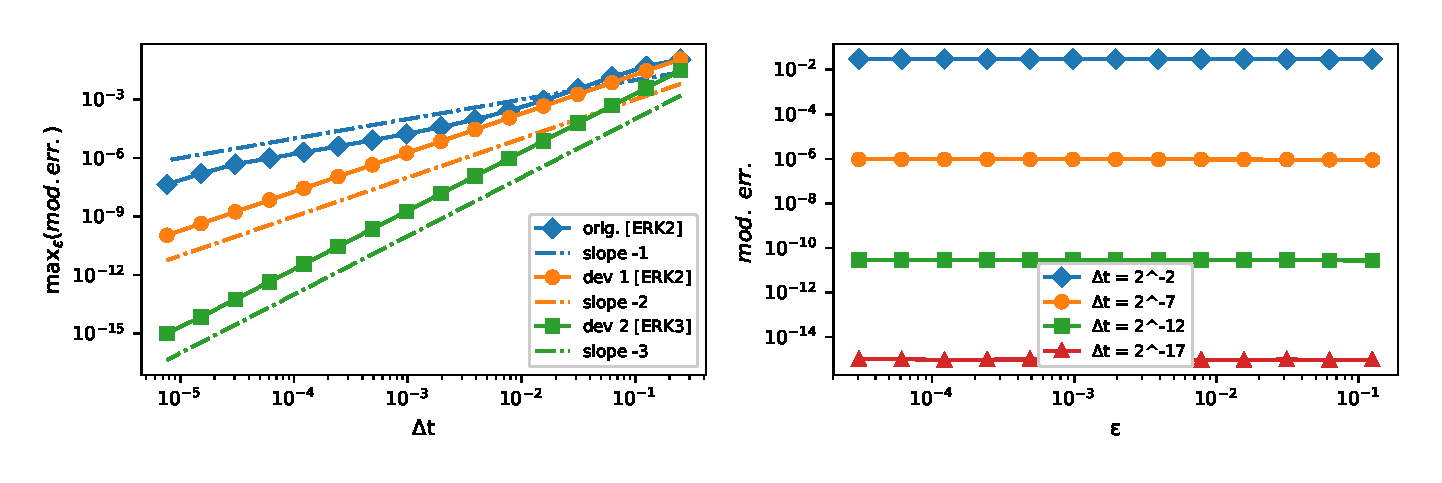
\includegraphics[width=\textwidth]{./miMa_Dissipatif/cv_oscill_max_err_and_dev2.eps}
\vspace*{-24pt}
\caption{Oscillating case: On the left, maximum error on~$\eps$ (for $\eps
= 2^{-k}$ with $k$ spanning $\{3, \ldots, 15\}$) as a function of $\Dt$
when using exponential RK schemes (abbr. ERK) of different orders. On the
right, the error as a function of $\eps$ when solving the micro-macro
problem of order~2 using ERK3.}
\label{tests_fig:oscill}
\end{figure}


\medskip
\noindent\textit{A PDE-inspired problem}\\
%
Consider a problem similar to a relaxed conservation law (as in the next
subsection) but without transport, written
\begin{equation*}
  \left\lbrace\begin{array}{ll} 
    \dot u = \tilde{u} , 
    & u(0) \in \R^{d} , \displaystyle \vphantom{\int} 
    \\ \displaystyle
    \dot{\tilde{u}} = \frac{1}{\e} \big( g(u) - \tilde{u} \big) ,
    & \tilde{u}(0) \in \R^{d} 
  \end{array}\right.
\end{equation*}
for some smooth map $g: \R^{d} \mapsto \R^{d}$. This can be
transformed in a system of the form~\eqref{intro-eq:xz_pb} by setting~$x =
u$ and $z = g(u) - \tilde{u}$, yielding the problem 
\begin{equation} \label{sec:tests:eq:hyperb_ode}
  \left\lbrace\begin{array}{ll} \displaystyle \vphantom{\int}
    \dot x = g(x) - z , 
    & x(0) = u(0) , \\ \displaystyle
    \dot z = -\frac{1}{\e} z + g'(x) \big( g(x) - z \big) ,
    & z(0) = g(u(0)) - \tilde{u}(0) .
  \end{array}\right.
\end{equation}
The change of variable and vector field can be computed by hand up
to order~1,
\begin{equation*}
  \Omega\rk{1}_{\tau}(x,z) = \begin{pmatrix}
    x + \e e^{-\tau} z \\
    e^{-\tau} z + \e g'(x) g(x)
  \end{pmatrix} ,
\end{equation*}
\begin{equation*}
  F\rk{1}(x,z) = \begin{pmatrix}
    g(x) - \e g'(x) g(x) 
    \\
    - g'(x) z + \e \big(g'(x)^2 + g''(x)g(x) 
    - \e g''(x)g'(x)g(x) \big) z
  \end{pmatrix} .
\end{equation*}
Going to a higher order requires specific computations, as the expression
of $\frac{1}{\e} (\dpt + \Lambda) \Omega\rk 2 _\tau(x,z)$ is verbose and
involves for instance $g(x + \e e^{-\tau}z) - g(x)$. 
It can be checked by hand that this expression involves no~$e^{-\tau
\Lambda}$-term with the above expressions of $\Omega\rk 1$ and $F\rk 1$.
For numerical testing, we chose~$g(x) = -x^3/3$, $u(0) = 1$ and
$\tilde{u}(0) = 0$. The micro-macro problem was computed up to order~2. 

\begin{figure}
  \vspace*{-12pt}
  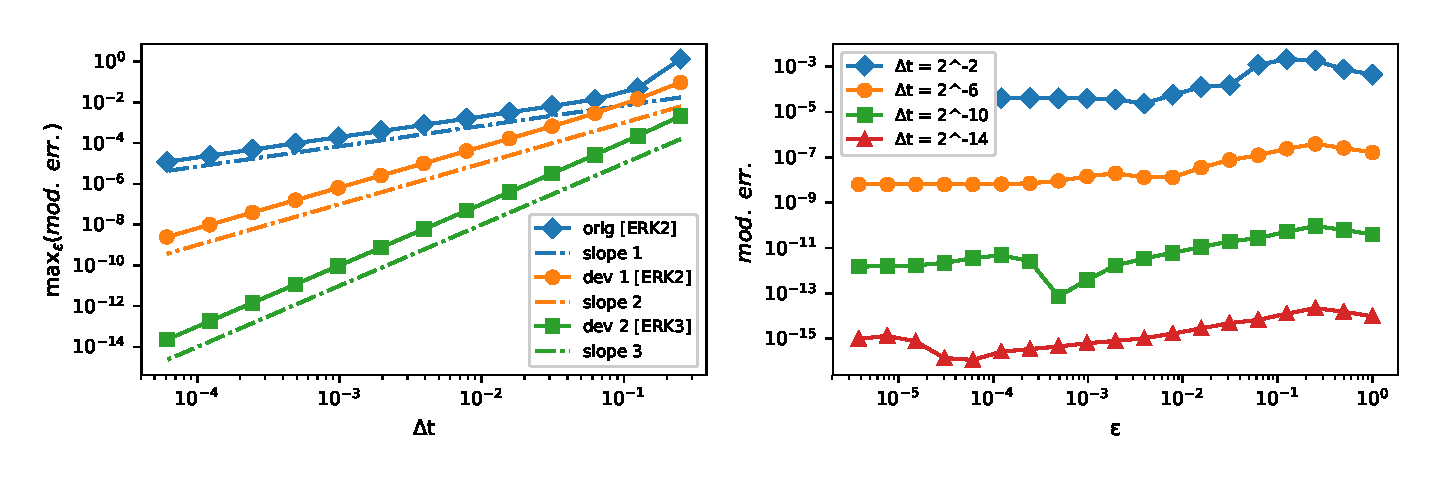
\includegraphics[width=\textwidth]{./miMa_Dissipatif/hyperb_ode.eps}
  \vspace*{-24pt}
  \caption{PDE-inspired problem: On the left, maximum error on~$\eps$ (for
  $\eps = 2^{-k}$ with $k$ spanning $\{1, \ldots, 18\}$) as a function of
  $\Dt$ when using exponential RK schemes (abbr. ERK) of different orders.
  On the right, the error as a function of $\eps$ when solving the
  micro-macro problem of order~2 using ERK3.}
  \label{tests_fig:hyperb_ode}
\end{figure}

\medskip
\noindent\textit{Results}\\
%
Figures~\ref{tests_fig:oscill} and~\ref{tests_fig:hyperb_ode} showcase the
phenomenon of order reduction when solving the original
problem~\eqref{test-pb:xz_oscil}: Despite using a scheme of order 2, the
error depends of $\eps$ in such a way that there exists no constant $C$
such that the error is bounded by $C\Dt^2$ for all $\eps$. However there
exists $C$ such that the error is bounded by $C\Dt$. In that case, we
cannot say that the error is of \textit{uniform} order~2, as this would
require the error to be independent of $\eps$.

This order reduction disappears when solving the micro-macro problem, as
can be seen on the right-hand side of the figures for a decomposition of
order 2. Furthermore, the theoretical orders of convergence from
Theorem~\ref{sec:mima:subsec:ua:thm:ua} are confirmed. Indeed, using a
scheme of order 2 (resp. 3) on the micro-macro problem of order 1 (resp.
2) generates a uniform error of the expected order of convergence, with no
order reduction. 



\subsection{Discretized hyperbolic partial differential equations}
\label{sec:tests:subsec:pde}
\hspace*{1em}

\renewcommand{\xvar}{\rho}
\renewcommand{\zvar}{z}
\noindent\textit{The telegraph equation}\\
%
\begin{figure}
\centering
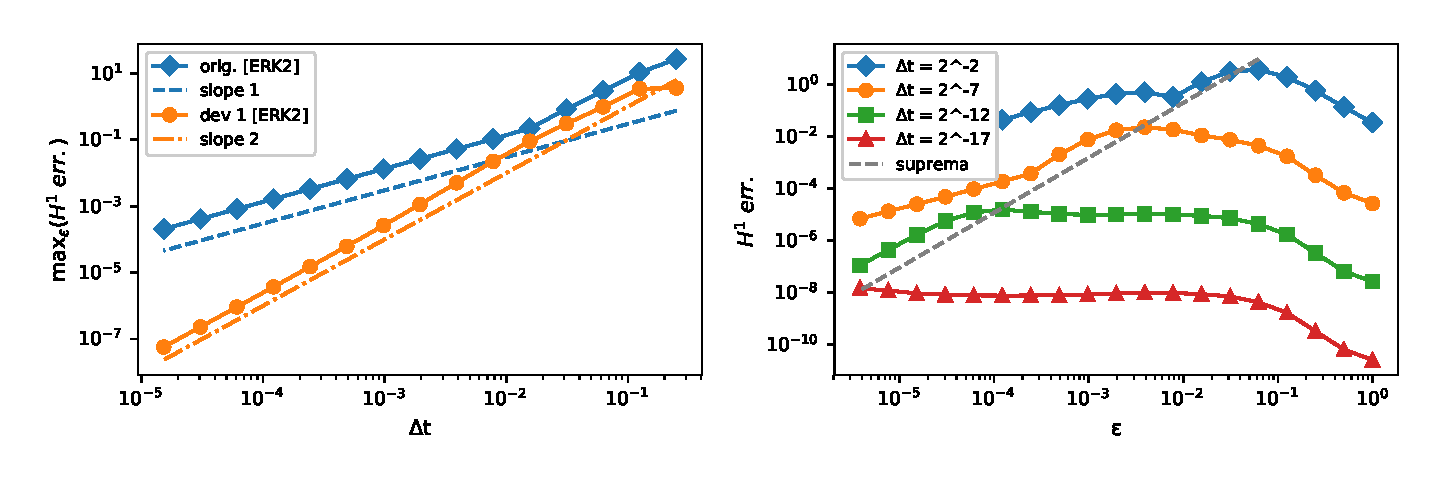
\includegraphics[width=\textwidth]{./miMa_Dissipatif/cv_telegraph_erk2.eps}
\vspace*{-24pt}
\caption{Telegraph equation: Absolute $H^1$ error on the solution of~\eqref{test_eq:cont_telegraph} computed by an ERK3 scheme. Supremum on $\eps$ as a function of $\Dt$ (left) and evolution of this error as a function of $\eps$ for the 1st-order decomposition (right). }
\label{test_fig:telegraph}
\end{figure}%
%
Using a spectral decomposition, we solve the problem, for $(t,x) \in [0,T] \times \R/2\pi\mathbb{Z}$, 
\begin{equation*} 
\left\{ \begin{array}{l}
\dpt \xvar + \dpx j = 0 , \\ \displaystyle
\dpt j + \frac{1}{\eps} \dpx \xvar = -\frac{1}{\eps} j , 
\end{array} \right. 
\end{equation*}
by setting $z = j + (1 - \alpha \eps \Delta)^{-1} \dpx z$, yielding 
problem~\eqref{pde_pb:telegraph}. The micro-macro decomposition of 
order~$1$ is summarized in Property~\ref{pde_prop:telegraph}, and its 
construction is detailed in Subsection~\ref{pde_subsec:telegraph}. 
%
Implementations are conducted using $\alpha = 2$, space frequencies are 
bounded by $k_{\max} := 12$, and initial data is $\xvar(0,x) = 
e^{\cos(x)}, \ j(0,x) = \frac{1}{2} \cos^3 (x)$. 

Results can be seen in Figure~\ref{test_fig:telegraph} when using a scheme
of order 2. When solving the original problem, the uniform order
degenerates from~2 to~1. When considering the micro-macro problem, the
order of convergence is not reduced and stays of order~2. Although it
varies with $\eps$ when considering a fixed $\Dt$, when considering the
supremum on~$\e$, there is no order reduction. The dashed slope on the
right plot interpolates the position of the supremum of the error for each
fixed $\Dt$. While the error seems to improve for $\e \ll \Dt$, this does
not cause any order reduction. This is stronger than the property of
preservation of asymptotes (which ERK schemes have,
see~\cite{dimarco.2011.exponential}), since AP schemes only need to be
well-defined in the limit $\e \rightarrow 0$. For them, this supremum does
not need to be bounded.
%
It appears that the relationship between the error bound and the stiffness
of the linear operator is rather complex when using exponential RK schemes
(again, see~\cite{hochbruck.2005.explicit} for details). 



\renewcommand{\Dx}{\Delta x}
\renewcommand{\rlxcont}{\tilde{u}}
\renewcommand{\rlxdisc}{\tilde{U}}
\renewcommand{\xvar}{U_1}
\renewcommand{\zvar}{U_2}
\medskip
\noindent\textit{Relaxed conservation law}\\
%
\begin{figure}
\centering
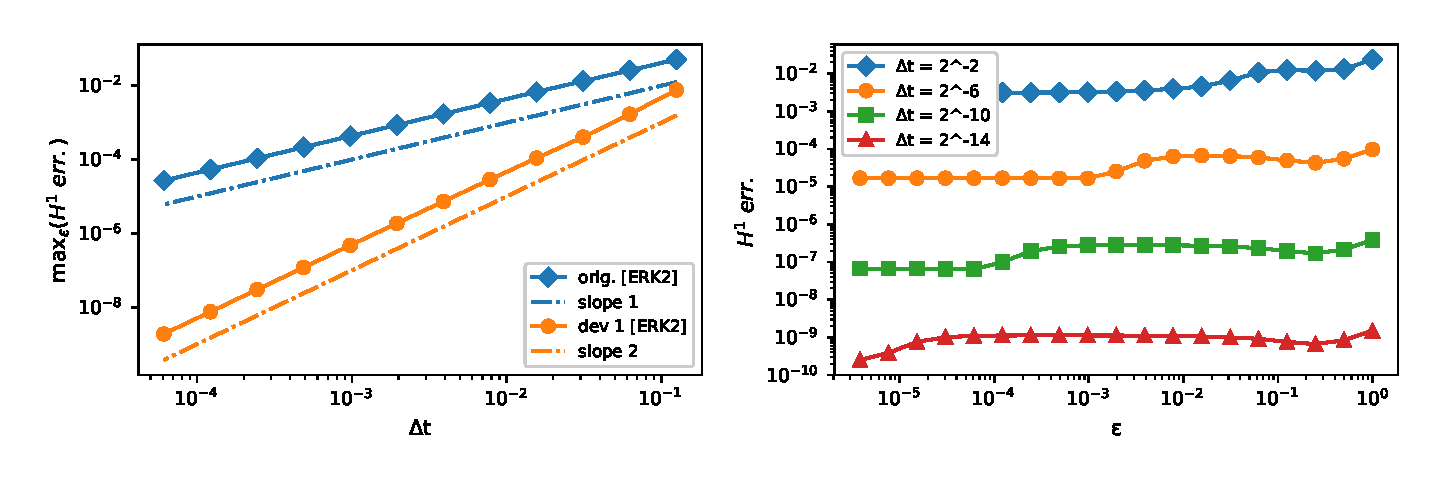
\includegraphics[width=\textwidth]{./miMa_Dissipatif/cv_hyperb_erk2.eps}
\vspace*{-24pt}
\caption{Relaxed Burgers-type problem: Maximum modified $H^1$ error (for $\eps$ spanning $1$ to $2^{-18}$ using an ERK3 scheme as a function of $\Dt$ (left), and $H^1$ error as a function of $\eps$ for the micro-macro problem of order~1 (right).}
\label{test_fig:sqr_results}
\end{figure}%
%
Our second test case is a hyperbolic problem for $(t,x) \in [0,T] \times \R/2\pi \mathbb Z$, 
\begin{equation*} %\label{test_eq:cont_hyperb_uv}
\left\{ \begin{array}{l}
\dpt u + \dpx \rlxcont = 0 , \\ \displaystyle
\dpt \rlxcont + \dpx u = \frac{1}{\eps}(g(u) - \rlxcont) ,
\end{array} \right .
\end{equation*}
discretized with finite volumes and written in the form of~\eqref{intro-eq:xz_pb} 
by setting $u_1 = u$ and $u_2 = \tilde{u} - g(u)$ 
the $x\eeps$- and the $z\eeps$-component respectively. 
The micro-macro expansion is computed to order~$1$ using the strategy detailed in Subsection~\ref{pde_subsec:conservation}. 

For our tests, following~\cite{hu.2021.uniform}, we consider 
$ g(u) = bu^2 $ 
with $b = 0.2$. 
Simulations run to a final time $T = 0.25$ and the mesh size is fixed: $N = 16$. 
Initial data is $u(0,x) = \frac{1}{2} e^{\sin(x)}$ and $\rlxcont(0,x) = \cos(x)$. 
The reference solution was computed up to a precision $10^{-12}$ using an ERK2 scheme. 
Convergence results are presented in Figure~\ref{test_fig:sqr_results}, 
confirming theoretical results once more. 

It should be said again that our approach does not study the error in space, only in time. 
For instance, the relationship between the error bound and the grid size is not considered. 
Further studies will be conducted, especially considering CFL conditions, $L^2$ and $H^1$ norms, and computational costs. 


\subsection{Thoughts} 
\label{sec:tests:subsec:thoughts}

\hspace*{1em}

\noindent\textit{Computing cost}\\
%
Note that when using a given scheme, solving a single step is much more
costly for the micro-macro problem than for the direct problem: Not only
is the system size doubled, but the functions implicated require more
computing power to obtain a single value (especially the defect,
see~\eqref{sec:pde:subsec:csv:eq:eta1} for instance). It is therefore 
plausible to think that our method is best for computing values during the
transient phase, after which it is possible to solve the original problem 
with uniform accuracy. 

The regularized derivation $\big( I_N - 2\eps D^2 \big)^{-1} D$ which
appears in the micro-macro problem of the relaxed hyperbolic system may be
prohibitively costly to compute for some schemes such as WENO, for which
the derivation operator is non-linear. However we may be able to work
around this, as the goal of the relaxation term is only to dampen
high-frequencies, and as such inverting any discrete Laplace operator
should suffice, independently of the scheme used to discretize the
transport. Clearly, the subject of utilizing such regularizations for
numerical purposes is complex and beyond the scope of this paper.


\medskip
\noindent\textit{Near-equilibrium convergence}\\
%
\begin{figure}
\centering
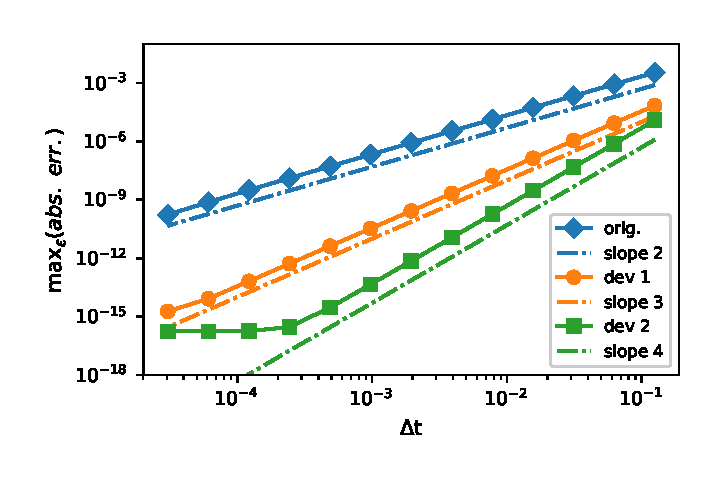
\includegraphics[width=0.48\textwidth]{./miMa_Dissipatif/ord_gain_oscill.eps}
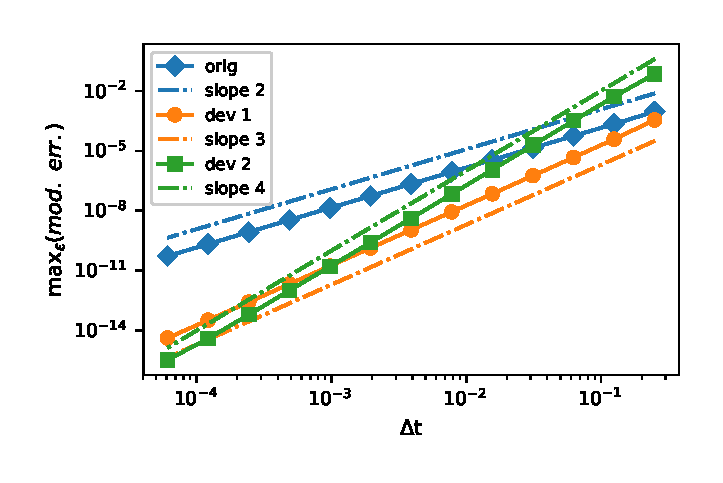
\includegraphics[width=0.48\textwidth]{./miMa_Dissipatif/ord_gain_hyperb_ode.eps}
\\
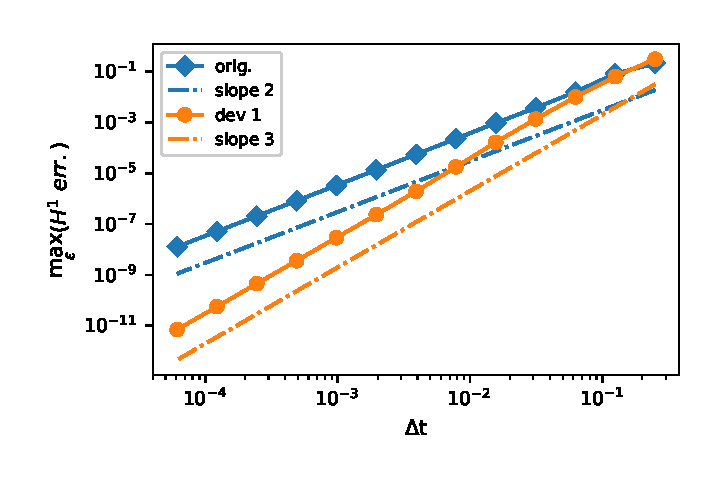
\includegraphics[width=0.48\textwidth]{./miMa_Dissipatif/ord_gain_telegraph.eps}
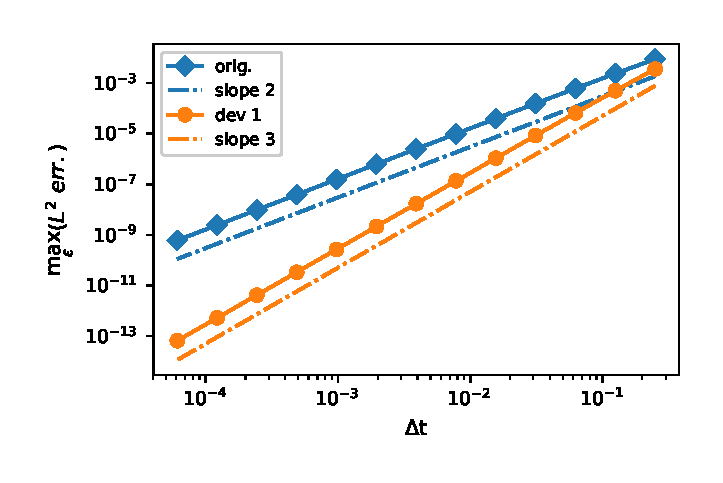
\includegraphics[width=0.48\textwidth]{./miMa_Dissipatif/ord_gain_cons_law.eps}
\vspace*{-10pt}
\caption{In reading order, errors when solving the oscillating toy
problem, the PDE-inspired problem, the telegraph equation and the relaxed
conservation law. All systems start near equilibrium and are solved with
exponential Runge-Kutta schemes of the observed order of convergence.}
\label{test_fig:order_gain}
\end{figure}%
%
If one chooses an initial condition $z\eeps(0) = 0$ in~\eqref{intro-eq:xz_pb}, 
then it is close to the center manifold up to $\bigO(\eps)$, 
and Problem~\eqref{intro-pb:full_pb_on_u} can be solved with uniform accuracy of order 2 
but only when considering the absolute error $|\cdot|$, 
not the modified error $\modnorm{\,\cdot\,}$ from~\eqref{mima_def:modnorm}. 
The same behaviour is observed for the telegraph equation when setting $j(0,x) = -\dpx \rho(0,x) $, meaning $z = \bigO(\eps)$. 
This would theoretically mean that we need to push the micro-macro 
decompositions up to order 2 if we want to improve the order of 
convergence. However, this is not the case: uniform accuracy of order 3 is 
obtained from an expansion of order 1 for all test cases. 
%
This ``order gain'' also propagates to our micro-macro decomposition of order~2 
for the oscillating toy problem. 
These results can be seen in Figure~\ref{test_fig:order_gain} 
and will be studied in future works. 


\clearemptydoublepage
\mainmatter

\clearemptydoublepage
\chapter{Discussion d'extension des résultats}

\section{Coût de calcul, erreurs d’arrondis, derivative-free, pullback}

Coût de calcul avec les non-linéarités

Difficulté du calcul de la relaxation pour certains schémas

Gain d’ordre avec $z(0) = 0$ (figure avec err sup sur $\varepsilon$)

Donner une clé pour le gain d’ordre : $v_z(0) = \mathcal{O}(\varepsilon)$


\section{Autour de l’équation de télégraphe}



\clearemptydoublepage
\backmatter\appendix
\chapter{Un développement double-échelle}
\label{chap:two-scale}

Résultats du stage et du début de thèse

\clearemptydoublepage

\chapter{Présentation de schémas exponentiels}
\label{chap:schemas}
\newcolumntype{C}{>{$}c<{$}}

On présente ici les schémas exponentiel Runge-Kutta utilisés en Chapitre~\ref{chap:dissip-mima}. Il ne s'agit pas de discuter des preuves de convergence des schémas, mais de fournir les outils nécessaires pour l'implémentation de ceux-ci. Tous les schémas décrits ici sont disponibles dans~\cite{hochbruck.2005.explicit}, on adapte seulement les notations de cet article au problème qui nous concerne, c'est-à-dire un problème de la forme
\begin{equation*}
    \pa_t u = -\frac{1}{\eps} A u + f(u), 
    \qquad 
    u(0) = u_0 \in \setR^d
\end{equation*}
avec $(-A)$ un qui engendre un semi-groupe $t \mapsto e^{-tA}$ uniformément borné pour $t \in \setR_+$ et $u \mapsto f(u)$ régulière. Il est à noter que dans~\cite{hochbruck.2005.explicit}, les auteurs mentionnent une problématique de réduction d'ordre. En particulier, ils décrivent les schémas de Cox \& Matthews dans~\cite{cox.2002.exponential} (d'ordres~3 et~4) comme pouvant entraîner une réduction à l'ordre~2 du fait d'un non-respect des conditions d'ordre des schémas. Cette notion est à distinguer de la réduction d'ordre qu'on observe en Introduction et en Chapitre~\ref{chap:dissip-mima}, qui provient d'une dégénérescence de l'erreur à cause des dérivées de la solution qui ne sont pas bornées.


Entre un temps $t_n$ et un temps $t_{n+1} = t_n + \Dt$, on considère qu'on dispose d'une approximation $u_n \approx u(t_n)$ et on cherche à trouver $u_{n+1} \approx u(t_{n+1})$. La méthode utilisé est un schéma de Runge-Kutta explicite exponentiel à~$s$ étages, qui peut s'écrire
\begin{align*}
& u_{n+1} = e^{-\Dt\, A/\eps} u_n + \Dt \sum_{i = 1}^s 
    b_i({\textstyle -\frac{\Dt}{\eps} A}) f(U_{ni}) ,
\\
& U_{ni} = e^{-c_i \Dt\, A/\eps} u_n + \Dt \sum_{j = 1}^{i-1} 
    a_{ij}({\textstyle -\frac{\Dt}{\eps} A}) f(U_{nj}),
\qquad
  i = 1, \ldots, s .
\end{align*}
La différence par rapport à un schéma standard est que les coefficients du schéma dépendent de l'opérateur $A$ qui est \enquote{filtré}. 

Étant donné que l'argument au sein des coefficients est toujours le même, on peut écrire ce schéma sous forme de tableau de Butcher, de la même manière que les méthodes de Runge-Kutta standards:
\begin{center}
    \begin{tabular}{C|CCCC}
           0    &    0    \\
          c_2   &  a_{21}   &     0     \\
        \vdots  &  \vdots   &  \ddots   &  \ddots   \\
          c_s   &  a_{s1}   &  \cdots   &  a_{s,s-1} & 0 \\ \hline
                & b_1       &  \cdots   &  \cdots    & b_s 
    \end{tabular}
\end{center}
Par exemple la méthode d'Euler explicite exponentielle
\begin{equation*}
    u_{n+1} = e^{-\Dt\, A/\eps} u_n 
        + \left( 
            \int_0^{\Dt} e^{(\Dt - \tau) A/\eps} \D\tau 
        \right) f(u_n)
\end{equation*}
devient sous forme de tableau, en définissant $\varphi_1(-hA) = h^{-1} \int_0^{h} e^{(h-\tau)A} \D\tau$,
\begin{center}
    \begin{tabular}{C|C}
        0 & 0 \\ \hline
          & \varphi_1
    \end{tabular}
\end{center}
avec le raccourci $\varphi_1 = \varphi_1(-\frac{\Dt}{\eps}A)$.
%
Pour les tableaux suivants, on définit 
\begin{equation*}
    \varphi_j(-hA) = h^{-j} 
        \int_0^h \frac{\tau^{j-1}}{(j-1)!} e^{(h-\tau)A} \D\tau ,
\end{equation*}
ce qui correspond au reste intégral renormalisé dans le développement de l'exponentiel. De sorte à avoir des coefficients dont l'argument est toujours $-\frac{\Dt}{\eps} A$ dans les tableaux, on définit aussi 
\begin{equation*}
    \varphi_{i,j}(-hA) = \varphi_j(-c_i h A) .
\end{equation*}

On peut maintenant énoncer les tableaux de Butcher des schémas utilisés dans le Chapitre~\ref{chap:dissip-mima}. Le schéma d'ordre~2 est
\begin{center}
    \begin{tabular}{C|CC}
        0  \\
        \frac{1}{2} & \frac{1}{2}\varphi_{1,2} \\ \hline
        & \varphi_1 - 2\varphi_2 & 2\varphi_2
    \end{tabular}
\end{center}
Le schéma d'ordre~3 est celui de Cox et Matthews~\cite{cox.2002.exponential}, 
\begin{center}
    \begin{tabular}{C|CCC}
        0  \\
        \frac{1}{2} & \frac{1}{2}\varphi_{1,2} \\ 
        1 & -\varphi_{1,3} & 2\varphi_{1,3}
        \\ \hline
        & 4\varphi_3 - 3\varphi_2 + \varphi_1 
        & -8\varphi_3 + 4\varphi_2
        & 4\varphi_3 - \varphi_2
    \end{tabular}
\end{center}
de même que celui d'ordre~4,
\begin{center}
    \begin{tabular}{C|CCCC}
        0  \\
        \frac{1}{2} & \frac{1}{2}\varphi_{1,2} \\ 
        \frac{1}{2} & 0 & \frac{1}{2}\varphi_{1,3} \\
        1 & \frac{1}{3}\left(\varphi_{0,3} - 1\right) & 0 & \varphi_{1,3}
        \\ \hline
        & \varphi_1 - 3\varphi_2 + 4\varphi_3
        & 2\varphi_2 - 4\varphi_3
        & 2\varphi_2 - 4\varphi_3
        & 4\varphi_3 - \varphi_2
    \end{tabular}
\end{center}

% \clearpage
% Méthodes composées

% Tableaux de Butcher

% Spltting

% \todo[inline]{Stormer-Verlett est un cas particulier de Strang mélangé à Euler explicite. En effet avec $\dot q = v$ et $\dot v = F(q)$,}
% \vspace*{-2\bigskipamount}
% \begin{align*}
% &   v_{n + 1/2} = v_n + \frac{\Dt}{2}F(q_n) \\
% &   q_{n+1} = q_n + \Dt\: v_{n+1/2} \\
% &   v_{n+1} = v_{n+1/2} + \frac{\Dt}{2}F(q_{n+1}) .
% \end{align*}
% \vspace*{-\medskipamount}
% \todo[inline]{Ce qui revient à séparer le système en $\pa_t (q,v) = (0, F(q))$ et $\pa_t (q,v) = (v, 0)$.}




\clearemptydoublepage
\chapter{Autour de notions géométriques}

\section{Algèbre de Lie}

\section{Géométrie de la moyennisation stroboscopique}

\clearemptydoublepage

\clearemptydoublepage
\chapter{Titre du premier chapitre}

Lorem ipsum dolor sit amet, «~consectetuer~» adipiscing elit. Maecenas fermentum, elit non lobortis cursus, orci velit suscipit est, id mollis turpis mi eget orci. Ut aliquam sollicitudin metus. Mauris at sapien sed sapien congue iaculis. Nulla lorem urna, bibendum id, laoreet iaculis, nonummy eget, massa. Phasellus ullamcorper commodo velit. Class aptent taciti sociosqu ad litora torquent per «~conubia nostra~», per inceptos hymenaeos. Phasellus est. Maecenas felis augue, gravida quis, porta adipiscing, iaculis vitae, felis. Nullam ipsum. Nulla a sem ac leo fringilla mattis. Phasellus egestas augue in sem. Etiam ac enim non mauris ullamcorper scelerisque. In wisi leo, malesuada vulputate, tempor sit amet, facilisis vel, velit. Mauris massa est, sodales placerat, luctus id, hendrerit a, urna. Nullam eleifend pede eget odio. Duis non erat. Nullam pellentesque.

Lorem ipsum dolor sit amet, consectetuer adipiscing elit. Maecenas fermentum, elit non lobortis cursus, orci velit suscipit est, id mollis turpis mi eget orci. Ut aliquam sollicitudin metus. Mauris at sapien sed sapien congue iaculis. Nulla lorem urna, bibendum id, laoreet iaculis, nonummy eget, massa\footcite[12]{Pierre1901}. Phasellus ullamcorper commodo velit. Class aptent taciti sociosqu ad litora torquent per conubia nostra, per inceptos hymenaeos. Phasellus est. Maecenas felis augue, gravida quis, porta adipiscing, iaculis vitae, felis. Nullam ipsum. Nulla a sem ac leo fringilla mattis. Phasellus egestas augue in sem. Etiam ac enim non mauris ullamcorper scelerisque. In wisi leo, malesuada vulputate, tempor sit amet, facilisis vel, velit. Mauris massa est, sodales placerat, luctus id, hendrerit a, urna. Nullam eleifend pede eget odio. Duis non erat. Nullam pellentesque. 

\section{Première section du chapitre}

\subsection{Première sous-section}

Cras molestie. Curabitur id urna. Suspendisse tempor. Aliquam erat
volutpat. Aliquam erat volutpat. Nam ultricies metus sit amet
erat\footnote{Mauris neque odio, ornare id, rhoncus non, sollicitudin
sed, lectus. Phasellus et dolor. Aenean ullamcorper risus id libero.
Pellentesque ac sem eget libero aliquam tincidunt. Suspendisse neque.}.
Suspendisse eget ipsum ut purus imperdiet suscipit. Mauris sed urna at
diam volutpat placerat. Nulla vitae tortor. Nulla sed nisl.

Lorem ipsum dolor sit amet, consectetuer adipiscing elit. Maecenas
fermentum, elit non lobortis cursus, orci velit suscipit est, id mollis
turpis mi eget orci. Ut aliquam sollicitudin metus. Mauris at sapien sed
sapien congue iaculis. Nulla lorem urna, bibendum id, laoreet iaculis,
nonummy eget, massa. Phasellus ullamcorper commodo velit. Class aptent
taciti sociosqu ad litora torquent per conubia nostra, per inceptos
hymenaeos. Phasellus est. Maecenas felis augue, gravida quis, porta
adipiscing, iaculis vitae, felis. Nullam ipsum. Nulla a sem ac leo
fringilla mattis. Phasellus egestas augue in sem. Etiam ac enim non
mauris ullamcorper scelerisque. In wisi leo, malesuada vulputate, tempor
sit amet, facilisis vel, velit. Mauris massa est, sodales placerat,
luctus id, hendrerit a, urna. Nullam eleifend pede eget odio. Duis non
erat. Nullam pellentesque\footcite[56]{Desfois1998}.


\begin{quote}
Aenean ullamcorper risus id libero. Pellentesque ac sem eget libero aliquam tincidunt. Suspendisse neque. Rutrum id, faucibus vitae, leo. Donec ut wisi. Vivamus ornare, lorem quis tristique dapibus, nulla nisl nonummy libero, vitae luctus sem felis vel nisl. Suspendisse lectus lacus, ultricies vitae, feugiat et, hendrerit in, quam. Pellentesque porttitor enim at lectus. Praesent viverra laoreet velit. Mauris neque odio, ornare id, rhoncus non, sollicitudin sed, lectus. Aenean ullamcorper risus id libero. Pellentesque ac sem eget libero aliquam tincidunt. Suspendisse neque\footcite[voir \pno~154]{Georges1974}.
\end{quote}



Morbi lorem. Etiam scelerisque rhoncus orci\footcite{Georges1974}. Nunc elementum ante ac leo. Vestibulum venenatis dictum nunc. Donec turpis est, dictum nec, fringilla nec, cursus id, quam. In nibh orci, porttitor ut, rutrum id, faucibus vitae, leo. Donec ut wisi. Vivamus ornare, lorem quis tristique dapibus, nulla nisl nonummy libero, vitae luctus sem felis vel nisl. Suspendisse lectus lacus, ultricies vitae, feugiat et, hendrerit in, quam. Pellentesque porttitor enim at lectus. Praesent viverra laoreet velit\footcite[56]{Desfois1998}. Mauris neque odio, ornare id, rhoncus non, sollicitudin sed, lectus. Phasellus et dolor. Aenean ullamcorper risus id libero. Pellentesque ac sem eget libero aliquam tincidunt. Suspendisse neque. Curabitur egestas neque ultrices nisl. Nulla bibendum augue et tellus. Duis ultrices convallis est.



Lorem ipsum dolor sit amet, consectetuer adipiscing elit. Maecenas fermentum, elit non lobortis cursus, orci velit suscipit est, id mollis turpis mi eget orci. Ut aliquam sollicitudin metus. Mauris at sapien sed sapien congue iaculis. Nulla lorem urna, bibendum id, laoreet iaculis, nonummy eget, massa. Phasellus ullamcorper commodo velit. Class aptent taciti sociosqu ad litora torquent per conubia nostra, per inceptos hymenaeos. Phasellus est. Maecenas felis augue, gravida quis, porta adipiscing, iaculis vitae, felis. Nullam ipsum. Nulla a sem ac leo fringilla mattis. Phasellus egestas augue in sem. Etiam ac enim non mauris ullamcorper scelerisque. In wisi leo, malesuada vulputate, tempor sit amet, facilisis vel, velit. Mauris massa est, sodales placerat, luctus id, hendrerit a, urna. Nullam eleifend pede eget odio. Duis non erat. Nullam pellentesque.

Lorem ipsum dolor sit amet, consectetuer adipiscing elit. Maecenas fermentum, elit non lobortis cursus, orci velit suscipit est, id mollis turpis mi eget orci. Ut aliquam sollicitudin metus. Mauris at sapien sed sapien congue iaculis. Nulla lorem urna, bibendum id, laoreet iaculis, nonummy eget, massa. Phasellus ullamcorper commodo velit. Class aptent taciti sociosqu ad litora torquent per conubia nostra, per inceptos hymenaeos. Phasellus est. Maecenas felis augue, gravida quis, porta adipiscing, iaculis vitae, felis. Nullam ipsum. Nulla a sem ac leo fringilla mattis. Phasellus egestas augue in sem. Etiam ac enim non mauris ullamcorper scelerisque. In wisi leo, malesuada vulputate, tempor sit amet, facilisis vel, velit. Mauris massa est, sodales placerat, luctus id, hendrerit a, urna. Nullam eleifend pede eget odio. Duis non erat. Nullam pellentesque.
Voir figure \ref{fig:mafigure2}.


\begin{figure}[htbp]
   \begin{center}
      \includegraphics[width=0.8\linewidth]{Chapitre1/figures/comparison.png}
   \end{center}
   \caption[titre court pour la liste des figures]
   {\footnotesize Titre plus long avec des explications.}
   \label{fig:mafigure2}
\end{figure}


\subsection{Deuxième sous-section}

Morbi lorem. Etiam scelerisque rhoncus orci. Nunc elementum ante ac leo. Vestibulum venenatis dictum nunc. Donec turpis est, dictum nec, fringilla nec, cursus id, quam. In nibh orci, porttitor ut, rutrum id, faucibus vitae, leo. Donec ut wisi. Vivamus ornare, lorem quis tristique dapibus, nulla nisl nonummy libero, vitae luctus sem felis vel nisl. Suspendisse lectus lacus, ultricies vitae, feugiat et, hendrerit in, quam. Pellentesque porttitor enim at lectus. Praesent viverra laoreet velit. Mauris neque odio, ornare id, rhoncus non, sollicitudin sed, lectus. Phasellus et dolor. Aenean ullamcorper risus id libero. Pellentesque ac sem eget libero aliquam tincidunt. Suspendisse neque. Curabitur egestas neque ultrices nisl. Nulla bibendum augue et tellus. Duis ultrices convallis est.

Lorem ipsum dolor sit amet, consectetuer adipiscing elit. Maecenas fermentum, elit non lobortis cursus, orci velit suscipit est, id mollis turpis mi eget orci. Ut aliquam sollicitudin metus. Mauris at sapien sed sapien congue iaculis. Nulla lorem urna, bibendum id, laoreet iaculis, nonummy eget, massa. Phasellus ullamcorper commodo velit. Class aptent taciti sociosqu ad litora torquent per conubia nostra, per inceptos hymenaeos. Phasellus est. Maecenas felis augue, gravida quis, porta adipiscing, iaculis vitae, felis. Nullam ipsum. Nulla a sem ac leo fringilla mattis. Phasellus egestas augue in sem. Etiam ac enim non mauris ullamcorper scelerisque. In wisi leo, malesuada vulputate, tempor sit amet, facilisis vel, velit. Mauris massa est, sodales placerat, luctus id, hendrerit a, urna. Nullam eleifend pede eget odio. Duis non erat. Nullam pellentesque.

Lorem ipsum dolor sit amet, consectetuer adipiscing elit. Maecenas fermentum, elit non lobortis cursus, orci velit suscipit est, id mollis turpis mi eget orci. Ut aliquam sollicitudin metus. Mauris at sapien sed sapien congue iaculis. Nulla lorem urna, bibendum id, laoreet iaculis, nonummy eget, massa. Phasellus ullamcorper commodo velit. Class aptent taciti sociosqu ad litora torquent per conubia nostra, per inceptos hymenaeos. Phasellus est. Maecenas felis augue, gravida quis, porta adipiscing, iaculis vitae, felis. Nullam ipsum. Nulla a sem ac leo fringilla mattis. Phasellus egestas augue in sem. Etiam ac enim non mauris ullamcorper scelerisque. In wisi leo, malesuada vulputate, tempor sit amet, facilisis vel, velit. Mauris massa est, sodales placerat, luctus id, hendrerit a, urna. Nullam eleifend pede eget odio. Duis non erat. Nullam pellentesque.

Lorem ipsum dolor sit amet, consectetuer adipiscing elit. Maecenas fermentum, elit non lobortis cursus, orci velit suscipit est, id mollis turpis mi eget orci. Ut aliquam sollicitudin metus. Mauris at sapien sed sapien congue iaculis. Nulla lorem urna, bibendum id, laoreet iaculis, nonummy eget, massa. Phasellus ullamcorper commodo velit. Class aptent taciti sociosqu ad litora torquent per conubia nostra, per inceptos hymenaeos. Phasellus est. Maecenas felis augue, gravida quis, porta adipiscing, iaculis vitae, felis. Nullam ipsum. Nulla a sem ac leo fringilla mattis. Phasellus egestas augue in sem. Etiam ac enim non mauris ullamcorper scelerisque. In wisi leo, malesuada vulputate, tempor sit amet, facilisis vel, velit. Mauris massa est, sodales placerat, luctus id, hendrerit a, urna. Nullam eleifend pede eget odio. Duis non erat. Nullam pellentesque.

Lorem ipsum dolor sit amet, consectetuer adipiscing elit. Maecenas fermentum, elit non lobortis cursus, orci velit suscipit est, id mollis turpis mi eget orci. Ut aliquam sollicitudin metus. Mauris at sapien sed sapien congue iaculis. Nulla lorem urna, bibendum id, laoreet iaculis, nonummy eget, massa. Phasellus ullamcorper commodo velit. Class aptent taciti sociosqu ad litora torquent per conubia nostra, per inceptos hymenaeos. Phasellus est. Maecenas felis augue, gravida quis, porta adipiscing, iaculis vitae, felis. Nullam ipsum. Nulla a sem ac leo fringilla mattis. Phasellus egestas augue in sem. Etiam ac enim non mauris ullamcorper scelerisque. In wisi leo, malesuada vulputate, tempor sit amet, facilisis vel, velit. Mauris massa est, sodales placerat, luctus id, hendrerit a, urna. Nullam eleifend pede eget odio. Duis non erat. Nullam pellentesque.

Lorem ipsum dolor sit amet, «~consectetuer~» adipiscing elit. Maecenas fermentum, elit non lobortis cursus, orci velit suscipit est, id mollis turpis mi eget orci. Ut aliquam sollicitudin metus. Mauris at sapien sed sapien congue iaculis. Nulla lorem urna, bibendum id, laoreet iaculis, nonummy eget, massa. Phasellus ullamcorper commodo velit. Class aptent taciti sociosqu ad litora torquent per «~conubia nostra~», per inceptos hymenaeos. Phasellus est. Maecenas felis augue, gravida quis, porta adipiscing, iaculis vitae, felis. Nullam ipsum. Nulla a sem ac leo fringilla mattis. Phasellus egestas augue in sem. Etiam ac enim non mauris ullamcorper scelerisque. In wisi leo, malesuada vulputate, tempor sit amet, facilisis vel, velit. Mauris massa est, sodales placerat, luctus id, hendrerit a, urna. Nullam eleifend pede eget odio. Duis non erat. Nullam pellentesque.

Lorem ipsum dolor sit amet, «~consectetuer~» adipiscing elit. Maecenas fermentum, elit non lobortis cursus, orci velit suscipit est, id mollis turpis mi eget orci. Ut aliquam sollicitudin metus. Mauris at sapien sed sapien congue iaculis. Nulla lorem urna, bibendum id, laoreet iaculis, nonummy eget, massa. Phasellus ullamcorper commodo velit. Class aptent taciti sociosqu ad litora torquent per «~conubia nostra~», per inceptos hymenaeos. Phasellus est. Maecenas felis augue, gravida quis, porta adipiscing, iaculis vitae, felis. Nullam ipsum. Nulla a sem ac leo fringilla mattis. Phasellus egestas augue in sem. Etiam ac enim non mauris ullamcorper scelerisque. In wisi leo, malesuada vulputate, tempor sit amet, facilisis vel, velit. Mauris massa est, sodales placerat, luctus id, hendrerit a, urna. Nullam eleifend pede eget odio. Duis non erat. Nullam pellentesque.

Lorem ipsum dolor sit amet, «~consectetuer~» adipiscing elit. Maecenas fermentum, elit non lobortis cursus, orci velit suscipit est, id mollis turpis mi eget orci. Ut aliquam sollicitudin metus. Mauris at sapien sed sapien congue iaculis. Nulla lorem urna, bibendum id, laoreet iaculis, nonummy eget, massa. Phasellus ullamcorper commodo velit. Class aptent taciti sociosqu ad litora torquent per «~conubia nostra~», per inceptos hymenaeos. Phasellus est. Maecenas felis augue, gravida quis, porta adipiscing, iaculis vitae, felis. Nullam ipsum. Nulla a sem ac leo fringilla mattis. Phasellus egestas augue in sem. Etiam ac enim non mauris ullamcorper scelerisque. In wisi leo, malesuada vulputate, tempor sit amet, facilisis vel, velit. Mauris massa est, sodales placerat, luctus id, hendrerit a, urna. Nullam eleifend pede eget odio. Duis non erat. Nullam pellentesque.


\section{Conclusion du premier chapitre}


Lorem ipsum dolor sit amet, consectetuer adipiscing elit. Maecenas fermentum, elit non lobortis cursus, orci velit suscipit est, id mollis turpis mi eget orci. Ut aliquam sollicitudin metus. Mauris at sapien sed sapien congue iaculis. Nulla lorem urna, bibendum id, laoreet iaculis, nonummy eget, massa. Phasellus ullamcorper commodo velit. Class aptent taciti sociosqu ad litora torquent per conubia nostra, per inceptos hymenaeos. Phasellus est. Maecenas felis augue, gravida quis, porta adipiscing, iaculis vitae, felis. Nullam ipsum. Nulla a sem ac leo fringilla mattis. Phasellus egestas augue in sem. Etiam ac enim non mauris ullamcorper scelerisque. In wisi leo, malesuada vulputate, tempor sit amet, facilisis vel, velit. Mauris massa est, sodales placerat, luctus id, hendrerit a, urna. Nullam eleifend pede eget odio. Duis non erat. Nullam pellentesque.



\clearemptydoublepage
\include{./Chapitre2/chapitre2}

\clearemptydoublepage
\backmatter
\include{./Conclusion/conclusion}

% Chapitre pour la bibliographie
% Bibliography chapter
\clearemptydoublepage
\phantomsection % To have a correct link in the table of contents
\addcontentsline{toc}{chapter}{Bibliography}

% nocite: Pour citer la totalit\'{e} des r\'{e}f\'{e}rences contenues dans le fichier biblio
% nocite: In order to cite all the references included biblio
\nocite{*}
\printbibliography[heading=primary,keyword=primary]
\newpage
\nocite{*}
\printbibliography[heading=secondary,keyword=secondary]

\clearemptydoublepage
% Pour avoir la quatrième de couverture sur une page paire
% To have the back cover on an even page
\cleartoevenpage[\thispagestyle{empty}]
\markboth{}{}
% Plus petite marge du bas pour la quatrième de couverture
% Shorter bottom margin for the back cover
\newgeometry{inner=30mm,outer=20mm,top=40mm,bottom=20mm}

%insertion de l'image de fond du dos (resume)
%background image for resume (back)
\backcoverheader

% Switch font style to back cover style
\selectfontbackcover{ % Font style change is limited to this page using braces, just in case

\titleFR{Méthodes d'analyse asymptotique et d'approximation numérique -- Problèmes d'évolution multi-échelles de type oscillatoire ou dissipatif}

\keywordsFR{décomposition micro-macro, précision uniforme, relaxation rapide, moyennisation}

\abstractFR{Les problèmes à relaxation rapide apparaissent dans de nombreux systèmes physiques ou biologiques, notamment dans le cadre de modèles cinétiques avec collisions. Leur comportement mélange une dynamique de relaxation de temps caractéristique $\eps$ et une partie lente d'interactions (généralement non-linéaire) ou de transport. Naturellement, on cherche à résoudre ce type de problème numériquement. Malgré le développement depuis les années 1980 de méthodes de résolution adaptées peu coûteuses (i.e. stables et essentiellement explicites), un problème demeure: la précision des méthodes est dégradée lorsque le pas de discrétisation est d'ordre~$\eps$. Dans ce manuscrit, on présente une méthode pour dépasser cette limite. L'approche mise en \oe{}uvre consiste à effectuer des développements asymptotiques par rapport au paramètre~$\eps$ de sorte à pouvoir séparer le modèle asymptotique et son erreur; on parle alors d'un problème micro-macro. Ce nouveau problème peut être résolu numériquement et on reconstruit la solution du problème d'origine avec une précision indépendante du paramètre~$\eps$. Nos développements asymptotiques font appel à des résultats récents de moyennisation, si bien qu'un chapitre de ce manuscrit est dédié à l'exposition de preuves originales de certains résultats de moyennisation connus. On discute en outre d'extensions possibles de nos résultats.}



\titleEN{Some methods for asymptotic analysis and numerical approximation -- Multi-scale evolution problems, of oscillatory or relaxation behavior}

\keywordsEN{micro-macro decomposition, uniform accuracy, stiff relaxation, averaging}

\abstractEN{Stiff relaxation problems appear in numerous physical and biological systems, most notably in kinetic models with collisions. The solutions of such problems present two dynamics which are intertwined: a relaxation of characteristic time~$\eps$, and a slow part of interactions or transport. Since the 1980s, efficient and stable methods have been developed to solve these problems numerically, however one issue remains: the accuracy of the method degrades when the time-step is of size~$\eps$. In this work, we present a method to overcome this limit. Our approach consists in performing asymptotic developments with relation to~$\eps$ to construct an \textit{non-stiff} asymptotic model and its error. We then consider this asymptotic behavior and the error separately -- this is a micro-macro decomposition. This new problem may be solved and the solution of the original problem recovered, all with an accuracy independent of~$\eps$. As our asymptotic developments use results from averaging, a chapter of this work is dedicated to averaging results. Specifically, we present original proofs of known results, using recent frameworks which make algebraic reasonings straightforward. A brief discussion surrounding possible extensions of our results is conducted at the end of the manuscript.}

}

% Rétablit les marges d'origines
% Restore original margin settings
\restoregeometry


\end{document}
